\باب{نظامِ تفرقی مساوات}
گزشتہ باب میں آپ نے بلند درجی سادہ تفرقی مساوات کو حل کرنا سیکھا۔اس باب میں سادہ تفرقی مساوات حل کرنے کا نیا طریقہ دکھایا جائے گا جس میں \عددی{n} درجی سادہ تفرقی مساوات سے \عددی{n} عدد درجہ اول سادہ تفرقی مساوات کا نظام حاصل کیا جائے گا۔اس نظام کو حل کرنا بھی سکھایا جائے گا۔تفرقی مساوات کے نظام کو قالب اور سمتیہ کی صورت میں لکھنا زیادہ مفید ثابت ہوتا ہے لہٰذا حصہ \حوالہ{حصہ_نظام_قالب} میں قالب اور سمتیہ کے بنیادی حقائق پر غور کیا جائے گا۔

اسی باب میں تفرقی مساوات کے نظام کو حل کرنے کی بجائے تمام مساوات کی مجموعی طرز عمل پر غور کیا جائے گا جس سے نظام کے حل کی \اصطلاح{استحکام}\فرہنگ{استحکام}\حاشیہب{stability}\فرہنگ{stability} کے بارے میں معلومات حاصل ہوتی ہے۔انجینئری میں مستحکم نظام  اہمیت رکھتے ہیں۔مستحکم نظام میں کسی لمحے پر معمولی تبدیلی، مستقبل کے لمحات پر معمولی تبدیلی ہی پیدا کرتی ہے۔اس ترکیب سے مساوات کا اصل حل دریافت نہیں ہوتا لہٰذا اس کو \اصطلاح{کیفی ترکیب}\فرہنگ{کیفی ترکیب}\فرہنگ{ترکیب!کیفی}\حاشیہب{qualitative method}\فرہنگ{qualitative method} کہتے ہیں۔جس ترکیب سے نظام کا اصل حل حاصل ہوتا ہو اس کو \اصطلاح{مقداری ترکیب}\فرہنگ{مقداری ترکیب}\فرہنگ{ترکیب!مقداری}\حاشیہب{quantitative method}\فرہنگ{quantitative method} کہتے ہیں۔

 
\حصہ{قالب اور سمتیہ کے بنیادی حقائق}\شناخت{حصہ_نظام_قالب}
تفرقی مساوات کے نظام پر غور کے دوران قالب اور سمتیات استعمال کئے جائیں گے۔

دو عدد خطی سادہ تفرقی مساوات کے نظام
\begin{gather}\label{مساوات_نظام_دو_مساوات}
\begin{aligned}
y_1' &=a_{11}y_1+a_{12}y_2\\
y_2' &=a_{21}y_1+a_{22}y_2
\end{aligned}\quad \text{یا} \quad
\begin{aligned}
y_1' &=2y_1-7y_2\\
y_2' &=5y_1+y_2
\end{aligned}
\end{gather}
 میں دو عدد نا معلوم تفاعل \عددی{y_1(t)} اور \عددی{y_2(t)} پائے جاتے ہیں۔ان مساوات میں دائیں جانب اضافی تفاعل \عددی{g_1(t)} اور \عددی{g_2(t)} بھی موجود ہو سکتے ہیں۔اسی طرح \عددی{n} عدد درجہ اول سادہ تفرقی مساوات پر مبنی نظام
\begin{gather}
\begin{aligned}\label{مساوات_نظام_متعدد_مساوات}
y_1' &=a_{11}y_1+a_{12}y_2+\cdots+a_{1n}y_n\\
y_2' &=a_{21}y_1+a_{22}y_2+\cdots a_{2n}y_n\\
\vdots &\\
y_n'&=a_{n1}y_1+a_{n2}y_2+\cdots+a_{nn}y_n
\end{aligned}
\end{gather}
 میں \عددی{y_1(t)} تا \عددی{y_n(t)} نا معلوم تفاعل پائے جائیں گے۔درج بالا ہر مساوات میں دائیں جانب اضافی تفاعل بھی پائے جا سکتے ہیں۔
%====================
\جزوحصہء{تکنیکی اصطلاحات}
\جزوحصہء{قالب}
نظام \حوالہ{مساوات_نظام_دو_مساوات} کے عددی سر (جو مستقل یا متغیرات ممکن ہیں) کو \عددی{2 \times 2} \اصطلاح{قالب}\فرہنگ{قالب}\حاشیہب{matrix}\فرہنگ{matrix} \bM{A} کی صورت میں لکھا جا سکتا ہے۔
\begin{gather}\label{مساوات_نظام_دو_جمع_دو_قالب}
\begin{aligned}
\bM{A}=[a_{jk}]=
\begin{bmatrix*}[r]
a_{11} & a_{12}\\
a_{21} & a_{22}
\end{bmatrix*}
\end{aligned}\quad \text{یا} \quad
\begin{aligned}
\bM{A}=[a_{jk}]=
\begin{bmatrix*}[r]
3 & 2\\
-1 &\frac{2}{3}
\end{bmatrix*}
\end{aligned}
\end{gather}
اسی طرح نظام \حوالہ{مساوات_نظام_متعدد_مساوات} کے عددی سر کو \عددی{n \times n} قالب کی صورت میں لکھا جا سکتا ہے۔
\begin{align}\label{مساوات_نظام_متعدد_جمع_متعدد_قالب}
\bM{A}=[a_{jk}]=
\begin{bmatrix*}[r]
a_{11} & a_{12} &\cdots & a_{1n}\\
a_{21} & a_{22}& \cdots & a_{2n}\\
& \vdots &  &\\
a_{n1} & a_{n2}& \cdots & a_{nn}
\end{bmatrix*}
\end{align}
قالب میں درج \عددی{a_{11}}، \عددی{a_{12}}، \عددی{a_{21}} وغیرہ کو \اصطلاح{ارکان}\فرہنگ{ارکان}\حاشیہب{entry}\فرہنگ{entry} کہتے ہیں۔ افقی لکیروں کو \اصطلاح{صف}\فرہنگ{صف}\حاشیہب{row}\فرہنگ{row} جبکہ عمودی لکیروں کو \اصطلاح{قطار}\فرہنگ{قطار}\حاشیہب{column}\فرہنگ{column} کہتے ہیں۔قالب \حوالہ{مساوات_نظام_دو_جمع_دو_قالب} میں پہلا صف \عددی{[a_{11} \,\,\,  a_{12}]} یا \عددی{[3\,\,\, 2]} جبکہ دوسرا صف \عددی{[a_{21} \,\,\,  a_{22}]} یا \عددی{[-1\,\,\,\tfrac{2}{3}]} ہے۔اسی طرح پہلا قطار درج ذیل ہے۔
\begin{gather*}
\begin{aligned}
\begin{bmatrix*}[r]
a_{11}\\
a_{21}
\end{bmatrix*}\quad \text{یا}\quad 
\begin{bmatrix*}[r]
3\\
-1
\end{bmatrix*}
\end{aligned}
\end{gather*}
ارکان کی علامتی اظہار میں دو گنا زیر نوشت کا پہلا عدد صف کو ظاہر کرتا ہے جبکہ دوسرا عدد قطار کو ظاہر کرتا ہے۔یوں \عددی{a_{21}} دوسری صف اور پہلی قطار کا رکن ہے۔ قالب \حوالہ{مساوات_نظام_دو_جمع_دو_قالب} کا \اصطلاح{مرکزی وتر}\فرہنگ{مرکزی وتر}\فرہنگ{وتر!مرکزی}\حاشیہب{main diagonal}\فرہنگ{diagonal!main} \عددی{a_{11}} اور \عددی{a_{22}} پر مبنی ہے جبکہ قالب \حوالہ{مساوات_نظام_متعدد_جمع_متعدد_قالب} کا مرکزی وتر \عددی{a_{11}}، \عددی{a_{22}}، \نقطے، \عددی{a_{nn}} پر مبنی ہے۔ہمیں یہاں صرف \اصطلاح{مربع قالب}\فرہنگ{مربع قالب}\فرہنگ{قالب!مربع}\حاشیہب{square matrix}\فرہنگ{matrix!square} درکار ہوں گے۔مربع قالب سے مراد ایسی قالب ہے جس میں صفوں کی تعداد قطاروں کی تعداد کے برابر ہو۔ قالب \حوالہ{مساوات_نظام_دو_جمع_دو_قالب} اور قالب \حوالہ{مساوات_نظام_متعدد_جمع_متعدد_قالب} مربع قالب ہیں۔

\اصطلاح{سمتیہ}۔\quad ایک قطار اور \عددی{n} ارکان کا \اصطلاح{سمتیہ قطار}\فرہنگ{سمتیہ!قطار}\فرہنگ{قطار!سمتیہ}\حاشیہب{column vector}\فرہنگ{vector!column} درج ذیل ہے۔
\begin{align*}
\bM{x}=
\begin{bmatrix*}[r]
x_1\\
x_2\\
x_3\\
\vdots\\
x_n
\end{bmatrix*}
\end{align*}
اسی طرح ایک صف اور \عددی{n} ارکان کا \اصطلاح{سمتیہ صف}\فرہنگ{سمتیہ صف}\فرہنگ{سمتیہ!صف}\حاشیہب{row vector}\فرہنگ{vector!row} درج ذیل ہے۔
\begin{align*}
\bM{v}=
\begin{bmatrix*}[r]
v_1 & v_2& v_3& \cdots & v_n
\end{bmatrix*}
\end{align*}
%=========================
\جزوحصہء{قالب اور سمتیات کا حساب}
\جزوحصہء{برابری مساوات} دو عدد \عددی{n \times n} قالب صرف اور صرف اس صورت برابر ہوں گے جب ان کے تمام \اصطلاح{نظیری}\فرہنگ{نظیری}\حاشیہب{corresponding}\فرہنگ{corresponding} ارکان \ترچھا{برابر} ہوں۔ظاہر ہے کہ دو قالب کی برابری کے لئے لازم ہے کہ ان میں صفوں کی تعداد یکساں ہو اور ان میں قطاروں کی تعداد یکساں ہو۔یوں \عددی{n=2} کی صورت میں 
\begin{align*}
\bM{A}=
\begin{bmatrix*}[r]
a_{11} & a_{12}\\
a_{21} & a_{22}
\end{bmatrix*} \quad \text{اور} \quad
\bM{B}=
\begin{bmatrix*}[r]
b_{11} & b_{12}\\
b_{21} & b_{22}
\end{bmatrix*}
\end{align*}
صرف اور صرف اس صورت برابر \عددی{(\bM{A}=\bM{B})} ہوں گے جب
\begin{align*}
a_{11}&=b_{11}, \quad a_{12}=b_{12}\\
a_{21}&=b_{21}, \quad a_{22}=b_{22}
\end{align*}
ہوں۔دو عدد سمتیہ صف (یا دو عدد سمتیہ قطار) صرف اور صرف اس صورت \ترچھا{برابر} ہوں گے جب دونوں میں ارکان کی تعداد  \عددی{n} برابر ہو اور  ان کے تمام نظیری  ارکان \ترچھا{برابر} ہوں ۔یوں 
\begin{align*}
\bM{v}=
\begin{bmatrix*}[r]
v_1\\
v_2
\end{bmatrix*} \quad \text{اور} \quad
\bM{x}=
\begin{bmatrix*}[r]
x_1\\
x_2
\end{bmatrix*}
\end{align*} 
کی صورت میں \عددی{\bM{v}=\bM{x}} صرف اور صرف تب ہو گا جب
\begin{align*}
v_1=x_1\quad \text{اور} \quad v_2=x_2
\end{align*}
ہوں۔

\جزوحصہء{مجموعہ} 
مجموعہ حاصل کرنے کی خاطر دونوں قالب کے نظیری ارکان کا مجموعہ لیا جاتا ہے۔دونوں قالب یکساں \عددی{m \times n} ہونا لازم ہے۔اسی طرح دونوں سمتیہ صف (یا دونوں سمتیہ قطار) میں برابر ارکان ہونا لازم ہے۔یوں \عددی{2 \times 2} قالب کا مجموعہ درج ذیل ہو گا۔
\begin{align}
\bM{A}+\bM{B}=
\begin{bmatrix*}[r]
a_{11}+b_{11} & a_{12}+b_{12}\\
a_{21}+b_{21}& a_{22}+b_{bb}
\end{bmatrix*}, \quad \bM{v}+\bM{x}=
\begin{bmatrix*}[r]
v_1+x_1\\
v_2+x_2
\end{bmatrix*}
\end{align} 
\جزوحصہء{غیر سمتی ضرب}\فرہنگ{غیر سمتی ضرب}\حاشیہب{scalar product}\فرہنگ{scalar product} غیر سمتی ضرب یعنی مستقل  \عددی{c} سے قالب کا ضرب حاصل کرنے کی خاطر قالب کے تمام ارکان کو \عددی{c} سے ضرب دیا جاتا ہے۔مثلاً 
\begin{align*}
\bM{A}=
\begin{bmatrix*}[r]
2& -3\\
5&1
\end{bmatrix*}, \quad 
-4\bM{A}=
\begin{bmatrix*}[r]
-8&12\\
-20&-4
\end{bmatrix*}
\end{align*}
اور
\begin{align*}
\bM{v}=
\begin{bmatrix*}[r]
9\\
-4
\end{bmatrix*}, \quad 
3\bM{v}=
\begin{bmatrix*}[r]
27\\
-12
\end{bmatrix*}
\end{align*}
\جزوحصہء{قالب ضرب قالب}
دو عدد \عددی{n \times n} قالب \عددی{\bM{A}=[a_{jk}]} اور \عددی{\bM{B}=[b_{jk}]}  کا حاصل ضرب \عددی{\bM{C}=\bM{A}\bM{B}}، (اسی ترتیب میں) \عددی{n \times n} قالب \عددی{\bM{C}=[c_{jk}]} ہو گا جس کے ارکان 
\begin{align}
c_{jk}=\sum_{m=1}^{n} a_{jm} b_{mk} \quad \quad j=1, \cdots, n, \quad\quad k=1,\cdots,n
\end{align}
ہوں گے یعنی \عددی{\bM{A}} قالب کے \عددی{j} صف کے ہر رکن کو \عددی{\bM{B}} قالب کے \عددی{j} قطار کے نظیری رکن کے ساتھ ضرب دیتے ہوئے \عددی{n} حاصل ضرب  کا مجموعہ لیں۔ہم کہتے ہیں کہ قالب کے ضرب سے مراد  \ترچھا{صف ضرب قطار} ہے۔مثلاً
\begin{align*}
\begin{bmatrix*}[r]
2 & 1\\
-3 & 0
\end{bmatrix*}
\begin{bmatrix*}[r]
7 &1\\
2&-4
\end{bmatrix*}=
\begin{bmatrix*}[r]
2\cdot 7+1\cdot 2& 2 \cdot 1+1\cdot(-4)\\
(-3)\cdot 7+0\cdot 2& (-3)\cdot 1+0\cdot(-4)
\end{bmatrix*}=
\begin{bmatrix*}[r]
16&-2\\
-21&-3
\end{bmatrix*}
\end{align*}
یہاں دھیان رہے  کہ ضرب قالب \اصطلاح{غیر مستبدل}\فرہنگ{مستبدل!غیر}\حاشیہب{non commutative}\فرہنگ{commutative!non} ہے لہٰذا  عموماً \عددی{\bM{A}\bM{B} \ne \bM{B}\bM{A}} ہو گا۔ یوں دو قالب کو آپس میں ضرب دیتے ہوئے  قالبوں کی ترتیب تبدیل نہیں کی جا سکتی۔اس حقیقت کی وضاحت کی خاطر درج بالا مثال میں قالبوں کی ترتیب بدلتے ہوئے ان کو آپس میں ضرب  دیتے ہیں۔
\begin{align*}
\begin{bmatrix*}[r]
7 & 1\\
2 & -4
\end{bmatrix*}
\begin{bmatrix*}[r]
2&1\\
-3&0
\end{bmatrix*}=
\begin{bmatrix*}[r]
7\cdot 2+1\cdot(-3)& 7\cdot 1+1\cdot 0\\
2\cdot 2+(-4)\cdot (-3)& 2\cdot 1 +(-4)\cdot 0
\end{bmatrix*}=
\begin{bmatrix*}[r]
11& 7\\
16 &2
\end{bmatrix*}
\end{align*}
\عددی{n \times n} قالب \عددی{\bM{A}} کو \عددی{n} ارکان کی سمتیہ قطار \عددی{\bM{x}} سے ضرب بھی اسی قاعدے کے تحت حاصل کی جاتی ہے۔یوں \عددی{\bM{v}=\bM{A}\bM{x}} کے \عددی{n} عدد ارکان درج ذیل ہوں گے۔
\begin{align}
v_j=\sum_{m=1}^{n} a_{jm}x_{m} \quad \quad j=1,\cdots, n
\end{align}
یوں
\begin{align*}
\begin{bmatrix*}[r]
7 & -3\\
1 & 4
\end{bmatrix*}
\begin{bmatrix*}[r]
x_1\\
x_2
\end{bmatrix*}=
\begin{bmatrix*}[r]
7x_1-3x_2\\
x_1+4x_2
\end{bmatrix*}
\end{align*}
ہو گا۔
%============================
\جزوحصہء{سادہ تفرقی مساوات کے نظام کا اظہار بذریعہ سمتیات}
\جزوحصہء{تفرق}
قالب یا سمتیہ کا تفرق، تمام ارکان کا تفرق حاصل کرنے سے حاصل ہوتا ہے۔
\begin{align*}
\bM{y}(t)=
\begin{bmatrix*}[r]
y_1(t)\\[0.5ex]
y_2(t)
\end{bmatrix*}=
\begin{bmatrix*}[r]
5t^3\\[0.5ex]
6\cos 2t
\end{bmatrix*},
\quad 
\bM{y}'(t)=
\begin{bmatrix*}[r]
y'_1(t)\\[0.5ex]
y'_2(t)
\end{bmatrix*}=
\begin{bmatrix*}[r]
15t^2\\[0.5ex]
-12\sin 2t
\end{bmatrix*}
\end{align*}
قالب کی تفرق اور ضرب کو استعمال کرتے ہوئے مساوات \حوالہ{مساوات_نظام_دو_مساوات} کو درج ذیل لکھا جا سکتا ہے۔ 
\begin{gather}
\begin{aligned}
\bM{y}'=
\begin{bmatrix*}[r]
y'_1\\[0.5ex]
y'_2
\end{bmatrix*}=\bM{A}\bM{x}=
\begin{bmatrix*}[r]
a_{11}& a_{12}\\[0.5ex]
a_{21}& a_{22}
\end{bmatrix*}
\begin{bmatrix*}[r]
y_1\\[0.5ex]
y_2
\end{bmatrix*}\quad \text{یا}\quad
\begin{bmatrix*}[r]
y'_1\\[0.5ex]
y'_2
\end{bmatrix*}=
\begin{bmatrix*}[r]
2&-7\\[0.5ex]
5&1
\end{bmatrix*}
\begin{bmatrix*}[r]
y_1\\[0.5ex]
y_2
\end{bmatrix*}
\end{aligned}
\end{gather}
اسی طرح مساوات \حوالہ{مساوات_نظام_متعدد_مساوات} کو  درج ذیل \عددی{\bM{y}=\bM{A}\bM{x}} صورت میں لکھا جا سکتا ہے۔
\begin{gather}
\begin{aligned}
\begin{bmatrix*}[r]
y_1'\\
y_2'\\
\vdots\\
y_n'
\end{bmatrix*}=
\begin{bmatrix*}[r]
a_{11}&a_{12}&\cdots &a_{1n}\\
a_{21}& a_{22}&\cdots &a_{2n}\\
&\vdots & &\\
a_{n1}&a_{n2}&\cdots &a_{nn}
\end{bmatrix*}
\begin{bmatrix*}[r]
y_1\\
y_2\\
\vdots\\
y_n
\end{bmatrix*}
\end{aligned}
\end{gather}
\جزوحصہء{مزید اعمال اور اصطلاحات}
\جزوحصہء{تبدیل محل} 
\اصطلاح{تبدیلی محل}\فرہنگ{تبدیلی محل}\حاشیہب{transposition}\فرہنگ{transposition} کے عمل سے قالب کے قطاروں کو صفوں کی جگہ لکھا جاتا ہے۔یوں \عددی{2\times 2} قالب \عددی{\bM{A}} سے \اصطلاح{تبدیلی محل}\فرہنگ{تبدیلی محل}\حاشیہب{transposition}\فرہنگ{transposition} کے ذریعہ \اصطلاح{تبدیلی محل قالب}\فرہنگ{تبدیلی محل قالب}\فرہنگ{قالب!تبدیلی محل}\حاشیہب{transpose matrix}\فرہنگ{transpose matrix} \عددی{\bM{A}^T} حاصل ہو گا۔ 
\begin{gather*}
\begin{aligned}
\bM{A}=
\begin{bmatrix*}[r]
a_{11} & a_{12}\\
a_{21}& a_{22}
\end{bmatrix*}=
\begin{bmatrix*}[r]
2&-11\\
4&3
\end{bmatrix*},\quad \quad
\bM{A}^T=
\begin{bmatrix*}[r]
a_{11}& a_{21}\\
a_{12}& a_{22}
\end{bmatrix*}=
\begin{bmatrix*}[r]
2 &4\\
-11&3
\end{bmatrix*}
\end{aligned}
\end{gather*}
سمتیہ صف \عددی{\bM{x}} کا تبدیلی محل سمتیہ \عددی{\bM{x}^T} سمتیہ قطار ہو گا۔اسی طرح سمتیہ قطار \عددی{\bM{v}} کا تبدیلی محل سمتیہ \عددی{\bM{v}^T} سمتیہ صف ہو گا۔
\begin{gather*}
\begin{aligned}
\bM{x}=
\begin{bmatrix*}[r]
x_1& x_2
\end{bmatrix*} \quad
\bM{x}^T=
\begin{bmatrix*}[r]
x_1\\
x_2
\end{bmatrix*}, \quad \quad
\bM{v}=
\begin{bmatrix*}[r]
v_1\\
v_2
\end{bmatrix*}\quad
\bM{v}^T=
\begin{bmatrix*}[r]
v_1 & v_2
\end{bmatrix*}
\end{aligned}
\end{gather*}
\جزوحصہء{قالب کا معکوس}
 ایسا \عددی{n \times n} قالب جس کے مرکزی وتر کے تمام ارکان اکائی \عددی{(1)}  اور بقایا  ارکان صفر ہوں کو \اصطلاح{اکائی قالب}\فرہنگ{اکائی قالب}\حاشیہب{unit matrix}\فرہنگ{unit matrix} \عددی{\bM{I}} کہتے ہیں۔
\begin{align}
\bM{I}=
\begin{bmatrix*}[r]
1&0 &0 & \cdots &0\\
0&1&0&\cdots & 0\\
0&0&1&\cdots &0\\
\vdots &&&&\\
0&0&0&\cdots&1
\end{bmatrix*}
\end{align}
ایسا \عددی{\bM{B}} قالب، جس کا \عددی{\bM{A}} قالب کے ساتھ حاصل ضرب اکائی قالب ہو \عددی{\bM{B}\bM{A}=\bM{B}\bM{A}=\bM{I}}،   قالب \عددی{\bM{A}} کا معکوس قالب کہلاتا ہے جسے \عددی{\bM{A}^{-1}} لکھا جاتا ہے جبکہ ایسی صورت میں \عددی{\bM{A}} \اصطلاح{غیر نادر قالب}\فرہنگ{غیر نادر قالب}\فرہنگ{قالب!غیر نادر}\حاشیہب{non singular matrix}\فرہنگ{matrix!non singular} کہلاتا ہے۔یہاں \عددی{\bM{A}} اور \عددی{\bM{B}} دونوں \عددی{n \times n} قالب ہیں۔
\begin{align}
\bM{A}^{-1}\bM{A}=\bM{A}\bM{A}^{-1}=\bM{I}
\end{align}
قالب \عددی{\bM{A}} کا معکوس تب پایا جاتا ہے جب \عددی{\bM{A}} کا \اصطلاح{مقطع} غیر صفر\عددی{\abs{\bM{A}}\ne 0} ہو۔اگر \عددی{\bM{A}} کا معکوس نہ پایا جاتا ہو تب \عددی{\bM{A}} \اصطلاح{نادر}\فرہنگ{نادر!قالب}\فرہنگ{قالب!نادر}\حاشیہب{singular}\فرہنگ{singular!matrix}\فرہنگ{matrix!singular} قالب کہلاتا ہے۔ مربع \عددی{2 \times 2} قالب کا معکوس
\begin{align}
\bM{A}^{-1}=\frac{1}{\abs{\bM{A}}}
\begin{bmatrix*}[r]
a_{22}& -a_{12}\\
-a_{21}& a_{22}
\end{bmatrix*}
\end{align}
ہے جہاں \عددی{\bM{A}} کا مقطع \عددی{\abs{\bM{A}}} درج ذیل ہے۔
\begin{align}
\abs{\bM{A}}=
\begin{vmatrix}
a_{11}&a_{12}\\
a_{21}&a_{22}
\end{vmatrix}=a_{11}a_{22}-a_{12}a_{21}
\end{align}
\جزوحصہء{خطی طور تابعیت}
\عددی{r} عدد سمتیات \عددی{\bM{v}^{(1)}} تا \عددی{\bM{v}^{(r)}} جہاں ہر سمتیہ \عددی{n} ارکان پر مشتمل ہو، اس صورت \اصطلاح{خطی طور غیر تابع سلسلہ}\فرہنگ{خطی طور!غیر تابع سلسلہ}\فرہنگ{سلسلہ!خطی طور غیر تابع}\حاشیہب{linearly independent set}\فرہنگ{linearly!independent set}\فرہنگ{set!linearly independent} یا \اصطلاح{خطی طور غیر تابع} کہلاتے ہیں جب
\begin{align}\label{مساوات_نظام_خطی-طور_غیر_تابع_قالب}
c_1\bM{v}^{(1)}+\cdots+c_r \bM{v}^{(r)}=\bM{0}
\end{align}
سے مراد  \عددی{c_1} تا \عددی{c_r} کی قیمتیں صفر ہو۔درج بالا مساوات میں \عددی{\bM{0}} \اصطلاح{صفر سمتیہ}\فرہنگ{صفر سمتیہ}\فرہنگ{سمتیہ!صفر}\حاشیہب{zero vector}\فرہنگ{zero vector} ہے جس کے تمام \عددی{n} ارکان صفر کے برابر ہیں۔اگر مساوات \حوالہ{مساوات_نظام_خطی-طور_غیر_تابع_قالب} میں \عددی{c_1} تا \عددی{c_r} کوئی ایک یا ایک سے زائد مستقل غیر صفر ہوں تب \عددی{\bM{v}^{(1)}} تا \عددی{\bM{v}^{(r)}} \اصطلاح{خطی طور تابع سلسلہ}\فرہنگ{خطی طور!تابع سلسلہ}\فرہنگ{سلسلہ!خطی طور تابع}\حاشیہب{linearly dependent vector}\فرہنگ{linearly dependent vector} یا \اصطلاح{خطی طور تابع} کہلائیں گے چونکہ ایسی صورت میں کم از کم ایک سمتیہ کو بقایا سمتیات کی مدد سے لکھا جا سکتا ہے، مثلاً \عددی{c_1 \ne 0} کی صورت میں مساوات \حوالہ{مساوات_نظام_خطی-طور_غیر_تابع_قالب} کو \عددی{c_1} سے تقسیم کرتے ہوئے
\begin{align*}
\bM{v}^{(1)}=-\frac{1}{c_1}\left[c_2\bM{v}^{(2)}+\cdots+c_r \bM{v}^{(r)}\right]
\end{align*}

لکھا جا سکتا ہے۔

\جزوحصہء{آئگنی قدر اور آئگنی سمتیات}
\اصطلاح{آئگنی قدر}\فرہنگ{آئگنی!قدر}\حاشیہب{Eigenvalues}\فرہنگ{Eigenvalues} اور \اصطلاح{آئگنی سمتیات}\فرہنگ{آئگنی!سمتیات}\حاشیہب{Eigenvectors}\فرہنگ{Eigenvectors} انتہائی اہم ہیں جو \اصطلاح{کوانٹم میکانیات}\فرہنگ{کوانٹم میکانیات}\حاشیہب{quantum mechanics}\فرہنگ{quantum mechanics} میں  کلیدی کردار ادا کرتے ہیں۔مساوات
\begin{align}\label{مساوات_نظام_آئگنی_الف}
\bM{A}\bM{x}=\lambda \bM{x}
\end{align}
میں \عددی{\bM{A}=[a_{jk}]} معلوم \عددی{n \times n} قالب ہے جبکہ  \عددی{\lambda} نا معلوم مستقل (جو حقیقی یا مخلوط مقدار ہو سکتا ہے) اور \عددی{\bM{x}} نا معلوم  سمتیہ ہے جنہیں حاصل کرنا درکار ہے۔کسی بھی \عددی{\lambda} کے لئے مساوات \حوالہ{مساوات_نظام_آئگنی_الف} کا ایک حل \عددی{\bM{x}=\bM{0}} ممکن ہے۔ایسی \اصطلاح{غیر سمتی}\فرہنگ{غیر سمتی!مقدار}\حاشیہب{scalar}\فرہنگ{scalar}  \عددی{\lambda} جو \عددی{\bM{x} \ne \bM{0}} کی صورت میں مساوات \حوالہ{مساوات_نظام_آئگنی_الف} پر پورا اترتی ہو، \عددی{\bM{A}} کی \اصطلاح{آئگنی قدر}\فرہنگ{آئگنی قدر}\حاشیہب{Eigenvalue}\فرہنگ{Eigenvalue} کہلاتی ہے جبکہ،  اس \عددی{\lambda} کی نظیری، \عددی{\bM{x}} کو  \عددی{\bM{A}} کی  \اصطلاح{آئگنی سمتیہ}\فرہنگ{آئگنی سمتیہ}\حاشیہب{Eigenvector}\فرہنگ{Eigenvector} کہتے ہیں۔

ہم مساوات \حوالہ{مساوات_نظام_آئگنی_الف} کو \عددی{\bM{A}\bM{x}-\lambda\bM{x}=0} یا 
\begin{align}\label{مساوات_نظام_آئگنی_ب}
(\bM{A}-\lambda \bM{I})\bM{x}=\bM{0}
\end{align}
لکھ سکتے ہیں جو \عددی{n} عدد خطی الجبرائی مساوات کو ظاہر کرتی ہے جس کے نا معلوم متغیرات \عددی{x_1} تا \عددی{x_n}، سمتیہ \عددی{\bM{x}} کے ارکان ہیں۔اس مساوات کے غیر صفر حل \عددی{\bM{x} \ne \bM{0}} کے لئے ضروری ہے کہ \عددی{\bM{A}-\bM{I}} کے عددی سر قالب کا \اصطلاح{مقطع} صفر ہو۔(یہ خطی الجبرا کی بنیادی حقیقت ہے)۔ اس باب میں ہمیں  \عددی{n=2} سے دلچسپی ہے لہٰذا مساوات \حوالہ{مساوات_نظام_آئگنی_ب} کو
\begin{align}\label{مساوات_نظام_آئگنی_پ}
\begin{bmatrix*}
a_{11}-\lambda& a_{12}\\
a_{21}& a_{22}-\lambda
\end{bmatrix*}
\begin{bmatrix*}
x_1\\
x_2
\end{bmatrix*}=
\begin{bmatrix*}[r]
0\\
0
\end{bmatrix*}
\end{align}
لکھتے ہیں جو درج ذیل مساوات کو ظاہر کرتی ہے۔
\begin{gather}\label{مساوات_نظام_آئگنی_ت}
\begin{aligned}
(a_{11}-\lambda)x_1+a_{12}x_2&=0\\
a_{21}x_1+(a_{22}-\lambda)x_2&=0
\end{aligned}
\end{gather}
اب نادر قالب کا \اصطلاح{مقطع} صفر ہوتا ہے لہٰذا \عددی{\bM{A}-\lambda\bM{I}}  اس صورت نادر قالب ہو گا جب اس قالب کا مقطع (جسے \عددی{\bM{A}} کی \اصطلاح{امتیازی مقطع}\فرہنگ{امتیازی!مقطع}\حاشیہب{characteristic determinant}\فرہنگ{characteristic determinant} کہتے ہیں) صفر ہو۔
\begin{gather}\label{مساوات_نظام_آئگنی_ٹ}
\begin{aligned}
\abs{\bM{A}-\lambda \bM{I}}&=
\begin{vmatrix}
a_{11}-\lambda& a_{12}\\
a_{21}& a_{22}-\lambda
\end{vmatrix}\\
&=(a_{12}-\lambda)(a_{22}-\lambda)-a_{12}a_{21}\\
&=\lambda^2-(a_{11}+a_{22})\lambda+a_{11}a_{22}-a_{12}a_{21}=0
\end{aligned}
\end{gather}
اس دو درجی مساوات کو \عددی{\bM{A}} کی \اصطلاح{امتیازی مساوات}\فرہنگ{امتیازی!مساوات}\حاشیہب{characteristic equation}\فرہنگ{characteristic!equation} کہتے ہیں۔اس کے حل \عددی{\lambda_1} اور \عددی{\lambda_2}، قالب \عددی{\bM{A}} کے آئگنی قدر یا آئگنی قیمتیں ہیں۔پہلے آئگنی قدر حاصل کریں۔اس کے بعد \عددی{\lambda_1} کو مساوات \حوالہ{مساوات_نظام_آئگنی_ت} میں پر کرتے ہوئے، \عددی{\lambda_1} کی نظیری، \عددی{\bM{A}} کی آئگنی سمتیہ \عددی{\bM{x}^{(1)}} دریافت کریں۔اسی طرح \عددی{\lambda_2} کو مساوات \حوالہ{مساوات_نظام_آئگنی_ت} میں پر کرتے ہوئے، \عددی{\lambda_2} کی نظیری، \عددی{\bM{A}} کی آئگنی سمتیہ \عددی{\bM{x}^{(2)}} دریافت کریں۔یاد رہے کہ اگر \عددی{\bM{x}} قالب \عددی{\bM{A}} کا آئگنی سمتیہ ہو تب \عددی{k\bM{x}} بھی \عددی{\bM{A}} کا آئگنی سمتیہ ہو گا جہاں \عددی{k \ne 0} ہے۔
%=========================

\ابتدا{مثال}
درج ذیل قالب کی آئگنی قیمتیں اور آئگنی سمتیات دریافت کریں۔
\begin{align*}
\bM{A}=
\begin{bmatrix*}[r]
-3& 3\\
-0.8&0.4
\end{bmatrix*}
\end{align*}
حل:امتیازی مساوات
\begin{align*}
\begin{vmatrix}
-3-\lambda&3\\
-0.8&0.4-\lambda
\end{vmatrix}=\lambda^2+2.6\lambda+1.2=0
\end{align*}
سے \عددی{\bM{A}} کے آئگنی قدر \عددی{\lambda_1=-0.6} اور \عددی{\lambda_2=-2} ملتے ہیں۔آئگنی قیمت \عددی{\lambda=\lambda_1=-0.6} کو مساوات \حوالہ{مساوات_نظام_آئگنی_ت} میں پر کرتے ہیں۔
\begin{gather*}
\begin{aligned}
(-3+0.6)x_1+3x_2&=0\\
-0.8x_1+(0.4+0.6)x_2&=0
\end{aligned}
\end{gather*}
پہلی مساوات کو \عددی{x_2=0.8x_1} لکھا جا سکتا ہے۔دوسری مساوات کو بھی \عددی{x_2=0.8x_1} لکھا جا سکتا ہے۔یوں اگر \عددی{x_1=1} چننا جائے تو \عددی{x_2=0.8}  ہو گا لہٰذا، \عددی{\lambda_1=-0.6} کی نظیری، \عددی{\bM{A}} کا آئگنی سمتیہ 
\begin{align*}
\bM{x}^{(1)}=
\begin{bmatrix*}[r]
1\\
0.8
\end{bmatrix*}
\end{align*}
ہو گا۔ اسی طرح \عددی{\lambda=\lambda_2=-2} کو مساوات \حوالہ{مساوات_نظام_آئگنی_ت} میں پر کرتے ہیں۔
\begin{gather*}
\begin{aligned}
(-3+2)x_1+3x_2&=0\\
-0.8x_1+(0.4+2)x_2&=0
\end{aligned}
\end{gather*}
ان دونوں مساوات کو \عددی{x_1=3x_2} لکھا جا سکتا ہے۔یوں اگر \عددی{x_2=1} چننا جائے تو \عددی{x_1=3} حاصل ہو گا لہٰذا، \عددی{\lambda_2=-2} کی نظیری، \عددی{\bM{A}} کا آئگنی سمتیہ 
\begin{align*}
\bM{x}^{(2)}=
\begin{bmatrix*}[r]
3\\
1
\end{bmatrix*}
\end{align*}
ہو گا۔جیسا پہلے ذکر کیا گیا، آئگنی سمتیات کو کسی  بھی غیر صفر عدد سے ضرب دیا جا سکتا ہے۔
\انتہا{مثال}
%============================

\حصہ{سادہ تفرقی مساوات کے نظام بطور انجینئری مسائل کے نمونے}
اس حصے میں ہم  تفرقی مساوات کے نظام کی عملاً اہمیت دیکھیں گے۔ ہم پہلے دیکھتے ہیں کہ ایسے نظام مختلف عملی مسائل میں کیسے کردار ادا کرتے ہیں۔ اس کے بعد ہم دیکھیں گے کہ بلند درجی تفرقی مساوات کو کیسے تفرقی مساوات کے نظام میں تبدیل کیا جا سکتا ہے۔
%====================

\ابتدا{مثال}\شناخت{مثال_نظام_ٹینکیوں_کا_نظام}\quad دو ٹینکیوں کا نظام\\
ایک ٹینکی کو استعمال کرتے ہوئے مرکب بنانے کے عمل پر صفحہ \حوالہصفحہ{مثال_سادہ_اول_مرکب} مثال \حوالہ{مثال_سادہ_اول_مرکب} میں غور کیا گیا جہاں مسئلے کو ایک عدد تفرقی مساوات سے ظاہر کیا گیا۔اس مثال کو ایک مرتبہ دیکھ لیں چونکہ وہی معلومات یہاں بھی استعمال کی جائیں گی۔
 
شکل \حوالہ{شکل_مثال_نظام_ٹینکیوں_کا_نظام} میں دو ٹینکیاں دکھائی گئی ہیں جن میں یک برابر دو سو \عددی{(200)} لٹر پانی موجود ہے۔ٹینکی الف میں خالص پانی ہے جبکہ ٹینکی ب کی پانی میں تیس \عددی{(30)} کلو گرام کا نمک ملایا گیا ہے۔ ٹینکیوں میں پانی کو مسلسل ہلایا جاتا ہے تا کہ ان میں ہر جگہ محلول یکساں رہے۔ٹینکیوں میں پانی کو چار \عددی{(4)} لٹر فی منٹ سے گردش دینے سے ٹینکی الف میں نمک کی مقدار \عددی{y_1(t)} اور ٹینکی ب میں نمک کی مقدار \عددی{y_2(t)} وقت کے ساتھ تبدیل ہوتی ہے۔کتنی دیر کے بعد ٹینکی الف میں نمک کی مقدار،  ٹینکی ب میں نمک کی مقدار کا نصف ہو گا؟
\begin{figure}
\centering
\begin{subfigure}{0.5\textwidth}
\centering
\begin{tikzpicture}
\draw(0,0) rectangle ++(-3/4*\x,\y);
\draw(\x,0) rectangle ++(3/4*\x,\y);
\draw(0,\y/4) rectangle ++(\x,\y/8);
\draw(0,3/4*\y) rectangle ++(\x,-\y/8);
\draw(-3/8*\x,\y/2)node[]{\RL{ٹینکی ب}};
\draw(\x+3/8*\x,\y/2)node[]{\RL{ٹینکی الف}};
\draw[-latex] (\x/4,\y/4+\y/16)--++(\x/2,0);
\draw[latex-] (\x/4,3/4*\y-\y/16)--++(\x/2,0);
\draw(\x/2,\y/4)node[below]{\RL{$4$ لٹر فی منٹ}};
\draw(\x/2,3/4*\y)node[above]{\RL{$4$ لٹر فی منٹ}};
\end{tikzpicture}
\end{subfigure}%
\begin{subfigure}{0.5\textwidth}
\centering
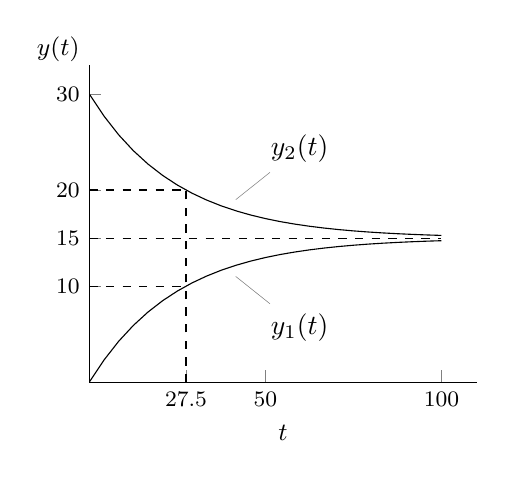
\begin{tikzpicture}
\begin{axis}[small,axis lines*=middle,xmin=0,ymin=0,xlabel={$t$},ylabel={$y(t)$},ylabel style={rotate=-90},ylabel style={at={(axis description cs:0,1.05)}},ytick={0,10,15,20,30},yticklabels={$0$,$10$,$15$,$20$,$30$},xtick={27.465,50,100},xticklabels={$27.5$,$50$,$100$}]
\addplot[domain=0:100]{15-15*e^(-0.04*x)}node[pos=0.4,pin=-45:{$y_1(t)$}]{};
\addplot[domain=0:100]{15+15*e^(-0.04*x)}node[pos=0.4,pin=45:{$y_2(t)$}]{};
\addplot[dashed] plot coordinates {(0,15)(100,15)};
\addplot[dashed] plot coordinates {(27.465,0)(27.465,20)};
\addplot[dashed] plot coordinates {(0,10)(27.465,10)};
\addplot[dashed] plot coordinates {(0,20)(27.465,20)};
\end{axis}
\end{tikzpicture}
\end{subfigure}%
\caption{ٹینکیوں کا نظام۔}
\label{شکل_مثال_نظام_ٹینکیوں_کا_نظام}
\end{figure}

حل:پہلا قدم:\quad نظام کی نمونہ کشی کرتے ہیں۔ ایک ٹینکی کی طرح، ٹینکی الف میں نمک کی مقدار \عددی{y_1(t)} میں تبدیلی کی شرح \عددی{y_1'(t)} نمک کی در آمدی اور بر آمدی شرح میں فرق کے برابر ہو گی۔  یہی کچھ \عددی{y_2'(t)} کے لئے بھی کہا جا سکتا ہے لہٰذا
\begin{align*}
y_1'&=4\frac{y_2}{200}-4\frac{y_1}{200}\\
y_2'&=4\frac{y_1}{200}-4\frac{y_2}{200}
\end{align*}
یعنی
\begin{align*}
y_1'&=-0.02 y_1+0.02y_2\\
y_2'&=\phantom{-}0.02y_1-0.02y_2
\end{align*}
ہو گا۔اس نظام کو
\begin{align}\label{مساوات_نظام_ٹینکی_الف}
\bM{y}'=\bM{A}\bM{y}
\end{align}
لکھا جا سکتا ہے جہاں
\begin{align*}
\bM{y}=
\begin{bmatrix*}[r]
y_1\\
y_2
\end{bmatrix*} \quad \text{اور} \quad 
\bM{A}=
\begin{bmatrix*}[r]
-0.02& \phantom{-}0.02\\
\phantom{-}0.02&-0.02
\end{bmatrix*}
\end{align*}
ہیں۔

دوسرا قدم:\quad عمومی حل حاصل کرتے ہیں۔ ایک عدد تفرقی مساوات کی طرح یہاں بھی حل کو قوت نمائی تفاعل
\begin{align}\label{مساوات_نظام_ٹینکی_ب}
\bM{y}=\bM{x}e^{\lambda t}
\end{align} 
فرض کرتے ہیں۔مساوات \حوالہ{مساوات_نظام_ٹینکی_الف} میں اس فرضی تفاعل اور اس کے تفرق کو پر کرتے ہیں۔
\begin{align*}
 \bM{y}'=\lambda \bM{x}e^{\lambda t}=\bM{A}\bM{x}e^{\lambda t}
\end{align*}
دونوں اطراف کو \عددی{e^{\lambda t}} سے تقسیم کرتے ہوئے دونوں اطراف کو بدل کر لکھتے ہیں۔
\begin{align*}
\bM{A} \bM{x}=\lambda \bM{x}
\end{align*}
ہمیں اس مساوات کے غیر صفر اہم حل درکار ہیں لہٰذا ہمیں \عددی{\bM{A}} کے آئگنی قدر اور آئگنی سمتیات حاصل کرنے ہوں گے۔آئگنی قدر امتیازی مساوات
\begin{align*}
\abs{\bM{A}-\lambda \bM{I}}=
\begin{vmatrix}
-0.02-\lambda& 0.02\\
0.02& -0.02-\lambda
\end{vmatrix}=
(-0.02-\lambda)-0.02^2=\lambda(\lambda+0.04)=0
\end{align*}
کے حل \عددی{\lambda_1=0} اور \عددی{\lambda_2=-0.04} ہوں گے۔(یہاں دھیان رہے کہ ہمیں غیر صفر آئگنی سمتیات درکار ہیں۔آئگنی قدر صفر ہو سکتے ہیں۔) آئگنی سمتیات مساوات \حوالہ{مساوات_نظام_آئگنی_ت} کے پہلے یا دوسرے مساوات سے حاصل ہوں گے۔مساوات \حوالہ{مساوات_نظام_آئگنی_ت} کی  پہلے مساوات کو استعمال کرتے ہوئے \عددی{\lambda_1=0} اور \عددی{\lambda_2=-0.04} کے لئے
\begin{align*}
-0.02x_1+0.02x_2=0, \quad (-0.02+0.04)x_1+0.02x_2=0
\end{align*}
لکھے جائیں گے جن سے \عددی{x_1=x_2} اور \عددی{x_1=-x_2} ملتے ہیں۔ہم \عددی{x_1=x_2=1} اور \عددی{x_1=-x_2=1} چنتے ہوئے \عددی{\lambda_1=0} اور \عددی{\lambda_2=-0.04} کے نظیری آئگنی سمتیات 
\begin{align*}
\bM{x}^{(1)}=
\begin{bmatrix*}[r]
1\\
1
\end{bmatrix*} \quad \text{اور} \quad
\bM{x}^{(2)}=
\begin{bmatrix*}[r]
1\\
-1
\end{bmatrix*}
\end{align*}
حاصل کرتے ہیں۔مساوات \حوالہ{مساوات_نظام_ٹینکی_ب} اور مسئلہ خطی میل (جو خطی متجانس تفرقی مساوات کے نظام پر بھی لاگو ہوتا ہے) کی مدد سے  حل لکھتے ہیں۔
\begin{align}\label{مساوات_نظام_ٹینکی_پ}
\bM{y}=c_1\bM{x}^{(1)}e^{\lambda_1 t}+c_2\bM{x}^{(2)}e^{\lambda_2 t}=c_1\begin{bmatrix*}[r] 1 \\ 1 \end{bmatrix*}+c_2 \begin{bmatrix*}[r] 1 \\ -1 \end{bmatrix*} e^{-0.04 t}
\end{align}
تیسرا قدم:\quad  ابتدائی معلومات \عددی{y_1(0)=0} (یعنی  ٹینکی الف میں ابتدائی طور پر کوئی نمک نہیں پایا جاتا)  اور \عددی{y_2(0)=30} (یعنی ٹینکی ب میں ابتدائی طور پر تیس کلو گرام نمک پایا جاتا ہے) ہیں۔مساوات \حوالہ{مساوات_نظام_ٹینکی_پ} میں \عددی{t=0} اور ابتدائی معلومات پر کرتے ہیں۔
\begin{align*}
\bM{y}(0)=c_1\begin{bmatrix*}[r] 1 \\ 1 \end{bmatrix*}+c_2 \begin{bmatrix*}[r] 1 \\ -1 \end{bmatrix*}=\begin{bmatrix*}[r] 0 \\ 30 \end{bmatrix*}
\end{align*}
درج بالا مساوات کی جزوی صورت \عددی{c_1+c_2=0} اور \عددی{c_1-c_2=30} ہے جس کا حل \عددی{c_1=15} اور \عددی{c_2=-15} ہے۔یوں ابتدائی معلومات پر پورا اترتا ہوا حل
\begin{align*}
\bM{y}=15\begin{bmatrix*}[r] 1 \\ 1 \end{bmatrix*}-15 \begin{bmatrix*}[r] 1 \\ -1 \end{bmatrix*} e^{-0.04 t}
\end{align*}
یعنی
\begin{align*}
y_1(t)&=15-15e^{-0.04 t}\\
y_2(t)&=15+15e^{-0.04 t}
\end{align*}
ہو گا۔اس حل کو شکل \حوالہ{شکل_مثال_نظام_ٹینکیوں_کا_نظام} میں دکھایا گیا ہے۔

چوتھا قدم: ٹینکی الف میں اس وقت ٹینکی ب کا آدھا نمک ہو گا جب اس میں \عددی{\tfrac{30}{3}=10} کلو گرام نمک ہو۔یوں درج ذیل حاصل ہوتا ہے۔
\begin{align*}
y_1(t)=15-15e^{-0.04 t}=10,\quad t=-\frac{1}{0.04}\ln \frac{1}{3}=\SI{27.5}{\minute}
\end{align*}

\انتہا{مثال}
%===============================
\ابتدا{مثال}\شناخت{مثال_نظام_برقی_جال}\quad برقی جال\\
شکل \حوالہ{شکل_مثال_نظام_برقی_جال} میں لمحہ \عددی{t=0} پر سوئچ چالو ہوتا ہے۔برقی رو \عددی{I_1(t)} اور \عددی{I_2(t)} دریافت کریں۔ابتدائی رو اور ابتدائی برقی گیر میں ذخیرہ بار صفر ہیں۔


\begin{figure}
\centering
\begin{tikzpicture}
\draw(0,0) to [american voltage source,l={${E=\SI{12}{\volt}}$}]++(0,\y) to [cspst,l={${t=0}$}]++(\x,0) to [inductor,l={${L=\SI{1}{\henry}}$}]++(\x,0) to [capacitor,l={${C=\SI{0.4}{\farad}}$}]++(\x,0) to [resistor,l={${R_2=\SI{5}{\ohm}}$}]++(0,-\y) to [short]++(-3*\x,0);
\draw(2*\x,0) to [resistor,*-*,l={${R_1=\SI{6}{\ohm}}$}]++(0,\y);
\draw[stealth-] ([shift={(-150:\x/4)}]3/4*\x,\y/2) arc (-150:150:\x/4);
\draw[stealth-] ([shift={(-150:\x/4)}]2*\x+\x/2,\y/2) arc (-150:150:\x/4);
\draw(3/4*\x,\y/2)node{$I_1$};
\draw(2*\x+\x/2,\y/2)node{$I_2$};
\end{tikzpicture}
\caption{مثال \حوالہ{مثال_نظام_برقی_جال} کا برقی جال۔}
\label{شکل_مثال_نظام_برقی_جال}
\end{figure}

حل:\موٹا{پہلا قدم} نظام کی نمونہ کشی ہے۔امالہ میں رو \عددی{I_1} ہے لہٰذا اس پر برقی دباو \عددی{v_L=L\tfrac{\dif I_1}{\dif t}} ہو گا۔برق گیر میں رو \عددی{I_2} ہے لہٰذا اس پر دباو \عددی{v_C=\tfrac{1}{C}\int I_2 \dif t} ہو گا۔مزاحمت \عددی{R_2} پر دباو \عددی{v_{R2}=I_2R_2} ہو گا جبکہ مزاحمت \عددی{R_1} میں کل رو \عددی{I_1-I_2} ہے لہٰذا اس پر دباو \عددی{v_{R1}=(I_1-I_2)R_1} ہو گا۔کرخوف قانون دباو کے تحت کسی بھی بند دائرے میں کل دباو کا اضافہ اس دائرے میں کل دباو کے گھٹاو کے برابر ہو گا۔یوں بائیں دائرے کے لئے
\begin{align*}
E=L\frac{\dif I_1}{\dif t}+(I_1-I_2)R_1
\end{align*}
لکھا جا سکتا ہے جس میں \عددی{E=12}، \عددی{L=1} اور \عددی{R_1=6} پر کرتے ہوئے
\begin{align}\label{مساوات_مثال_برقی_جال_الف}
I_1'=-6I_1+6I_2+12
\end{align}
ملتا ہے۔اسی طرح دائیں دائرے کے لئے
\begin{align*}
0=\frac{1}{C}\int I_2 \dif t+I_2R_2+(I_2-I_1)R_1
\end{align*}
لکھا جا سکتا ہے جس میں \عددی{C=0.4} اور \عددی{R_2=5} پر کرتے ہوئے تفرق لینے سے
\begin{align*}
I_2+4.4I_2'-2.4I_1'=0
\end{align*}
ملتا ہے۔اس میں مساوات \حوالہ{مساوات_مثال_برقی_جال_الف} سے \عددی{I_1'} کی قیمت پر کرتے ہوئے
\begin{align*}
I_2+4.4I_2'-2.4(-6I_1+6I_2+12)=0
\end{align*}
یعنی
\begin{align}\label{مساوات_مثال_برقی_جال_ب}
I_2'=-\frac{36}{11}I_1+\frac{67}{22}I_2+\frac{72}{11}
\end{align}
حاصل ہوتا ہے۔ مساوات \حوالہ{مساوات_مثال_برقی_جال_الف} اور مساوات \حوالہ{مساوات_مثال_برقی_جال_ب} کو 
\begin{align}\label{مساوات_نظام_برقی_غیر-متجانس_الف}
\bM{J}'=\bM{A} \bM{J}+\bM{g} 
\end{align}
لکھا جا سکتا ہے جہاں 
\begin{align*}
\quad \bM{J}=\begin{bmatrix*}[r] I_1 \\[0.5ex] I_2 \end{bmatrix*},\quad \bM{A}=\begin{bmatrix*}[r] -6 & 6\\[0.5ex] -\frac{36}{11}& \frac{67}{22} \end{bmatrix*}, \quad  \bM{g}=\begin{bmatrix*}[r] 12 \\[0.5ex] \frac{72}{11} \end{bmatrix*}
\end{align*}
ہیں۔\عددی{I_1'} اور \عددی{I_2'} کے  سمتیہ قطار کو \عددی{\bM{J}} اس لئے لکھا گیا ہے کہ اس باب میں \عددی{\bM{I}} اکائی قالب کے لئے استعمال کیا گیا ہے۔ 

\موٹا{دوسرا قدم} نظام کا حل تلاش کرنا ہے۔\عددی{\bM{g}} کی موجودگی  \ترچھا{غیر متجانس سادہ تفرقی نظام} کو ظاہر کرتی ہے لہٰذا ہم ایک عدد تفرقی مساوات کی طرح پہلے متجانس مطابقتی نظام \عددی{\bM{J}'=\bM{A}\bM{J}} کا حل حاصل کرتے ہیں۔ہم \عددی{\bM{J}=\bM{x}e^{\lambda t}} کو حل تصور کرتے ہوئے متجانس نظام میں پر کرتے ہوئے درج ذیل حاصل کرتے ہیں۔
\begin{align*}
\bM{J}'=\lambda \bM{x}e^{\lambda t}=\bM{A}\bM{x}e^{\lambda t} \quad \implies \quad \bM{A}\bM{x}=\lambda \bM{x}
\end{align*}
غیر صفر اہم حل کے حصول کے لئے \عددی{\bM{A}} کا آئگنی قدر اور آئگنی سمتیات درکار ہوں گے۔آئگنی قدر امتیازی مساوات
\begin{align*}
\abs{\bM{A}-\lambda \bM{I}}=\begin{vmatrix} -6-\lambda& 6 \\-\frac{36}{11}&\frac{67}{22}-\lambda \end{vmatrix}=\lambda^2+\frac{65}{22}\lambda-\frac{15}{11}=0
\end{align*}
سے \عددی{\lambda_1=-2.38209} اور \عددی{\lambda_2=-0.57245} حاصل ہوتے ہیں۔ان آئگنی قدر کی نظیری آئگنی سمتیات مساوات \حوالہ{مساوات_نظام_آئگنی_ت} سے حاصل ہوں گے۔مساوات \حوالہ{مساوات_نظام_آئگنی_ت} کے پہلے مساوات میں  \عددی{\lambda_1} پر کرتے ہوئے 
\begin{align*}
(-6+2.38209)x_1+6x_2&=0,\quad \implies x_1=1.658416x_2
\end{align*}
ملتا ہے۔یوں \عددی{x_2=1} چنتے ہوئے \عددی{x_1=1.658416} ملتا ہے جس سے \عددی{\bM{x}^{(1)}=\begin{bmatrix*} 1.658416 \\1  \end{bmatrix*}} حاصل ہوتا ہے۔اسی طرح مساوات \حوالہ{مساوات_نظام_آئگنی_ت} کے پہلے مساوات میں  \عددی{\lambda_2} پر کرتے ہوئے 
\begin{align*}
(-6+0.57245)x_1+6x_2&=0,\quad \implies x_1=1.105471x_2
\end{align*}
ملتا ہے۔یوں \عددی{x_2=1} چنتے ہوئے \عددی{x_1=1.105471} ملتا ہے جس سے \عددی{\bM{x}^{(2)}=\begin{bmatrix*} 1.105471 \\1  \end{bmatrix*}} حاصل ہوتا ہے۔یوں متجانس نظام کا عمومی حل درج ذیل ہو گا۔
\begin{align}
\bM{J}=c_1\bM{x}^{(1)}e^{\lambda_1 t}+c_2 \bM{x}^{(2)}e^{\lambda_2 t}
\end{align}
مساوات \حوالہ{مساوات_نظام_برقی_غیر-متجانس_الف} کے غیر متجانس نظام کا جبری تفاعل \عددی{\bM{g}} مستقل مقدار ہے لہٰذا اس نظام کا مخصوص حل  مستقل سمتیہ قطار \عددی{\bM{J}_p=\bM{a}} فرض کرتے ہیں جس کے ارکان \عددی{a_1} اور \عددی{a_2} ہیں۔ یوں \عددی{\bM{J}'=0} ہو گا۔ مساوات \حوالہ{مساوات_نظام_برقی_غیر-متجانس_الف} میں فرض کردہ مخصوص حل پر کرتے ہوئے  \عددی{\bM{A}\bM{a}+\bM{g}=0} ملتا ہے جو درج ذیل  مساوات کو ظاہر کرتی ہے۔
\begin{align*}
-6a_1+6a_2+12&=0\\
-\frac{36}{11}a_1+\frac{67}{22}a_2+\frac{72}{11}&=0
\end{align*}
ان ہمزاد مساوات کو حل کرنے سے \عددی{a_1=2} اور \عددی{a_2=0} ملتا ہے لہٰذا \عددی{\bM{a}=\begin{bmatrix*}[r] 2 \\ 0 \end{bmatrix*}} ہو گا۔یوں عمومی حل
\begin{align*}
\bM{J}=\bM{J}_h+\bM{J}_p=c_1\bM{x}^{(1)}e^{\lambda_1 t}+c_2 \bM{x}^{(2)}e^{\lambda_2 t}+\bM{a}
\end{align*}
ہو گا جو درج ذیل مساوات کو ظاہر کرتی ہے۔
\begin{align*}
I_1&=1.658416c_1e^{-2.38209 t}+1.105471c_2e^{-0.57245t}+2\\
I_2&=c_1e^{-2.38209t}+c_2e^{-0.57245t}
\end{align*}
ابتدائی معلومات کے تحت \عددی{I_1(0)=0} اور \عددی{I_2(0)=0} ہے۔انہیں درج بالا مساوات میں پر کرتے  ہوئے
\begin{align*}
1.658416c_1+1.105471c_2+2&=0\\
c_1+c_2&=0
\end{align*}
ملتا ہے جنہیں حل کرتے ہوئے \عددی{c_1=-3.61699} اور \عددی{c_2=3.61699} حاصل ہوتا ہے۔یوں مخصوص حل 
\begin{align*}
\bM{J}=-3.617\bM{x}^{(1)}e^{-2.38t}+3.617\bM{x}^{(2)}e^{-0.57t}+\bM{a}
\end{align*}
یعنی
\begin{align*}
I_1&=-5.998e^{-2.38 t}+3.998e^{-0.57t}+2\\
I_2&=-3.617e^{-2.38t}+3.617e^{-0.57t}
\end{align*}
ہو گا جسے شکل \حوالہ{شکل_مثال_نظام_برقی_جال_مخصوص_حل}-الف میں دکھایا گیا ہے۔
\begin{figure}
\centering
\begin{subfigure}{0.5\textwidth}
\centering
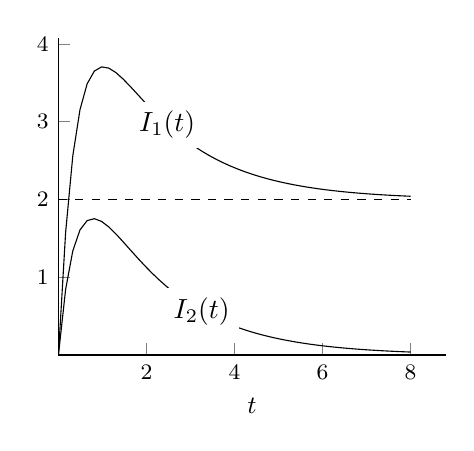
\begin{tikzpicture}
\begin{axis}[small,axis lines*=middle,xlabel={$t$},xmin=0,ymin=0]
\addplot[domain=0:8,samples=50]{-6*e^(-2.38*x)+4*e^(-0.57*x)+2}node[pos=0.5,fill=white]{$I_1(t)$};
\addplot[domain=0:8,samples=50]{-3.617*e^(-2.38*x)+3.617*e^(-0.57*x)}node[pos=0.5,fill=white]{$I_2(t)$};
\addplot[dashed] plot coordinates {(0,2) (8,2)};
\end{axis}
\end{tikzpicture}
\caption*{(الف) مثال \حوالہ{مثال_نظام_برقی_جال} کے دور کا مخصوص حل۔}
\end{subfigure}%
\begin{subfigure}{0.5\textwidth}
\centering
\begin{tikzpicture}
\begin{axis}[small,axis lines*=middle,xlabel={$I_1(t)$},ylabel={$I_2(t)$},xmin=0,xmax=3.9,ymin=0,ylabel style={rotate=-90},ylabel style={at={(axis description cs:0,1.05)}},xlabel style={at={(axis description cs:1.05,0)}}]
\addplot[domain=0:20,samples=150]({-6*e^(-2.38*x)+4*e^(-0.57*x)+2},{-3.617*e^(-2.38*x)+3.617*e^(-0.57*x)})coordinate[pos=0.5](ka)coordinate[pos=0.501](kb);
\draw[-stealth] (ka)--(kb);
\end{axis}
\end{tikzpicture}
\caption*{(ب) \عددی{I_1(t)} بالمقابل \عددی{I_2(t)}}
\end{subfigure}%
\caption{مثال \حوالہ{مثال_نظام_برقی_جال} کے منحنی۔}
\label{شکل_مثال_نظام_برقی_جال_مخصوص_حل}
\end{figure}

شکل \حوالہ{شکل_مثال_نظام_برقی_جال_مخصوص_حل}-ب میں \عددی{I_1(t)} بالمقابل \عددی{I_2(t)} کو \عددی{I_1 I_2} سطح پر دکھایا گیا ہے جس میں \عددی{t} مقدار معلوم  ہے۔مقدار معلوم کے بڑھنے کی سمت کو منحنی پر تیر کے نشان سے دکھایا گیا ہے۔ سطح \عددی{I_1 I_2} کو نظام کی \اصطلاح{سطح مرحلہ}\فرہنگ{سطح مرحلہ}\حاشیہب{phase plane}\فرہنگ{phase plane} کہتے ہیں جبکہ شکل \حوالہ{شکل_مثال_نظام_برقی_جال_مخصوص_حل}-ب کی منحنی کو \اصطلاح{خط حرکت}\فرہنگ{خط حرکت}\حاشیہب{trajectory}\فرہنگ{trajectory} کہتے ہیں۔ہم دیکھیں گے کہ \ترچھا{سطح مرحلہ اشکال}،  سادہ شکل \حوالہ{شکل_مثال_نظام_برقی_جال_مخصوص_حل}-الف طرز کے اشکال سے زیادہ اہم ثابت ہوتے ہیں۔یہ خطوط کی نسل کے بارے میں بہتر کیفی  معلومات فراہم کرتے ہیں۔
\انتہا{مثال}
%=============================

صفحہ \حوالہصفحہ{مثال_سادہ_اول_مرکب} مثال \حوالہ{مثال_سادہ_اول_مرکب} میں ایک عدد ٹینکی کی مثال پر غور کیا گیا جس کی نمونہ کشی ایک عدد سادہ تفرقی مساوات سے کی گئی۔ مثال \حوالہ{مثال_نظام_ٹینکیوں_کا_نظام} میں دو ٹینکیوں پر مبنی نظام کی نمونہ کشی  دو عدد تفرقی مساوات سے کی گئی۔ اسی طرح مثال \حوالہ{مثال_نظام_برقی_جال} میں دو عدد نا معلوم رو کی بنا دو عدد سادہ تفرقی مساوات حاصل ہوئے۔آپ دیکھ سکتے ہیں کہ زیادہ بڑے نظام کی نمونہ کشی زیادہ تعداد کی تفرقی مساوات سے کی جائے گی۔
%=======================

\جزوحصہء{\عددی{n} درجی سادہ تفرقی مساوات سے تفرقی مساوات کے نظام کا حصول}
درج ذیل مسئلہ میں ثابت کیا جاتا ہے کہ \عددی{n} درجی سادہ تفرقی مساوات \حوالہ{مساوات_بلند_درجی_سے_سادہ_الف} سے تفرقی مساوات کا نظام حاصل کیا جا سکتا ہے۔

\ابتدا{مسئلہ}\quad تفرقی مساوات کا مبادلہ\\
سادہ \عددی{n} درجی تفرقی مساوات
\begin{align}\label{مساوات_بلند_درجی_سے_سادہ_الف}
y^{(n)}=F(t,y,y',\cdots,y^{(n-1)})
\end{align}
میں
\begin{align}\label{مساوات_بلند_درجی_سے_سادہ_ب}
y_1=y,\quad y_2=y',\quad y_3=y'', \cdots, y_n=y^{(n-1)}
\end{align}
لے کر اس کو  \عددی{n} عدد سادہ ایک درجی تفرقی مساوات کے نظام
\begin{gather}
\begin{aligned}\label{مساوات_بلند_درجی_سے_سادہ_پ}
y_1'&=y_2\\
y_2'&=y_3\\
\vdots\\
y_{n-1}'&=y_n\\
y_n'&=F(t,y_1,y_2,\cdots,y_n)
\end{aligned}
\end{gather}
 میں تبدیل کیا جا سکتا ہے۔
\انتہا{مسئلہ}
%==========================
\ابتدا{ثبوت}
مساوات \حوالہ{مساوات_بلند_درجی_سے_سادہ_ب} کے تفرق سے نظام کے پہلے \عددی{n-1} عدد تفرقی مساوات حاصل ہوتے ہیں۔مساوات \حوالہ{مساوات_بلند_درجی_سے_سادہ_ب} سے \عددی{y_n'=y^{(n)}} بھی حاصل ہوتا ہے لہٰذا مساوات \حوالہ{مساوات_بلند_درجی_سے_سادہ_الف} سے مساوات \حوالہ{مساوات_بلند_درجی_سے_سادہ_پ} کی آخری مساوات بھی حاصل ہوتی ہے۔
\انتہا{ثبوت}
%============================

\ابتدا{مثال}\شناخت{مثال_نظام_اسپرنگ_کمیت}
ہم  اسپرنگ اور کمیت کی آزادانہ ارتعاش  کے مسئلے پر غور کر چکے ہیں جس کی تفرقی مساوات صفحہ \حوالہصفحہ{مساوات_سادہ_دو_درجی_قصری_نظام_الف} پر مساوات \حوالہ{مساوات_سادہ_دو_درجی_قصری_نظام_الف}
\begin{align}
my''+cy'+ky=0 \quad \implies \quad y''=-\frac{k}{m}y-\frac{c}{m}y'
\end{align}
 دیتی ہے جس کے لئے مساوات \حوالہ{مساوات_بلند_درجی_سے_سادہ_پ} کا نظام
\begin{align*}
y_1'&=y_2\\
y_2'&=-\frac{k}{m}y_1-\frac{c}{m}y_2
\end{align*}
 متجانس اور خطی ہے۔قالب کا استعمال کرتے ہوئے \عددی{\bM{y}=\begin{bmatrix*}[r] y_1 \\ y_2 \end{bmatrix*}} لکھتے ہوئے اس نظام کو درج ذیل لکھا جا سکتا ہے
\begin{align}
\bM{y}'=\bM{A}\bM{y}=\begin{bmatrix*}[r] 0 & 1 \\ -\frac{k}{m}& -\frac{c}{m} \end{bmatrix*}\begin{bmatrix*}[r]  y_1 \\ y_2 \end{bmatrix*}
\end{align}
جس سے امتیازی مساوات لکھتے ہیں۔
\begin{align*}
\abs{\bM{A}-\lambda \bM{I}}=\begin{vmatrix} -\lambda & 1\\ -\frac{k}{m}& -\frac{c}{m}-\lambda \end{vmatrix}=\lambda^2+\frac{c}{m}\lambda+\frac{k}{m}=0
\end{align*}
با مثلاً \عددی{m=1}، \عددی{c=1.4} اور \عددی{k=0.24} ہوں تب 
\begin{align*}
\lambda^2+1.4\lambda+0.24=(\lambda+0.2)(\lambda+1.2)=0
\end{align*}
ہو گا جس سے آئگنی قدر \عددی{\lambda_1=-0.2} اور \عددی{\lambda_2=-1.2} حاصل ہوتے ہیں۔آئگنی سمتیات \عددی{\bM{A}-\lambda \bM{I}=\bM{0}} کی پہلی مساوات \عددی{-\lambda x_1+x_2} سے حاصل کرتے ہیں۔آئگنی قدر \عددی{\lambda_1=-0.2} پر کرتے ہوئے  \عددی{0.2x_1+x_2=0} سے \عددی{x_2=-0.2x_1} ملتا ہے لہٰذا \عددی{x_1=1} چنتے ہوئے \عددی{x_2=-0.2} ہو گا۔اسی طرح \عددی{\lambda_2=-1.2} پر کرتے ہوئے \عددی{1.2x_1+x_2=0} سے \عددی{x_2=-1.2x_1} ملتا ہے لہٰذا \عددی{x_1=1} چنتے ہوئے \عددی{x_2=-1.2} ہو گا۔یوں درج ذیل آئگنی سمتیات حاصل ہوتی ہیں
\begin{align*}
\bM{x}^{(1)}=\begin{bmatrix*} 1 \\ -0.2  \end{bmatrix*}, \quad \bM{x}^{(2)}=\begin{bmatrix*}  1 \\ -1.2 \end{bmatrix*}
\end{align*}
جنہیں استعمال کرتے ہوئے
\begin{align*}
\bM{y}=c_1\begin{bmatrix*} 1 \\ -0.2  \end{bmatrix*}e^{-0.2 t}+c_2 \begin{bmatrix*}  1 \\ -1.2 \end{bmatrix*} e^{-1.2 t}
\end{align*}
سمتیہ حل لکھا جائے گا۔اس نظام کی پہلی مساوات
\begin{align*}
y=y_1=c_1e^{-0.2 t}+c_2e^{-1.2 t}
\end{align*}
درکار حل ہے جبکہ نظام کی دوسری مساوات حل کی تفرق ہے۔
\begin{align*}
y_2=y_1'=y'=-0.2c_1e^{-0.2 t}-1.2c_2e^{-1.2t}
\end{align*}
\انتہا{مثال}
%=================================

\حصہء{سوالات}
سوال \حوالہ{سوال_نظام_آئگنی_الف} تا سوال \حوالہ{سوال_نظام_آئگنی_ب} میں دیے گئے قالب کے آئگنی قدر اور آئگنی سمتیات حاصل کریں۔

%===================
\ابتدا{سوال}\شناخت{سوال_نظام_آئگنی_الف}
الیکٹران کی ایک خاصیت  \اصطلاح{چکر}\فرہنگ{چکر}\حاشیہب{spin}\فرہنگ{spin} کہلاتی ہے جس کی مقدار  \عددی{-\tfrac{\hbar}{2}} یا \عددی{\tfrac{\hbar}{2}} ہو سکتی ہے  جہاں \عددی{\hbar=\tfrac{h}{2\pi}} ہے اور \عددی{h=\SI{6.626e-34}{\meter^2\kilo\gram\per\second}} \اصطلاح{مستقل پلانک}\فرہنگ{مستقل پلانک}\حاشیہب{Plank's constant}\فرہنگ{Plank' constant}  ہے۔\اصطلاح{چکر} سمتیہ مقدار ہے۔مقناطیسی میدان میں الیکٹران کا \اصطلاح{چکر}  یا ہمہ میدان (مقناطیسی میدان کی سمت میں) رہتا ہے اور یا مخالف میدان (میدان کی الٹ سمت میں) رہتا ہے۔ہمہ میدان صورت میں الیکٹران کو \اصطلاح{اوپر چکر}\فرہنگ{اوپر چکر}\فرہنگ{اوپر چکر}\حاشیہب{spin up}\فرہنگ{spin up} الیکٹران کہتے ہیں جبکہ میدان مخالف چکر کی صورت میں  الیکٹران کو \اصطلاح{نیچے چکر}\فرہنگ{نیچے چکر}\حاشیہب{spin down}\فرہنگ{spin down} الیکٹران کہتے ہیں۔\عددی{z} سمت میں مقناطیسی میدان میں موجود الیکٹران کی خاصیت \عددی{\bM{S}_z} \اصطلاح{قالب چکر}\فرہنگ{قالب چکر}\حاشیہب{spin matrix}\فرہنگ{spin matrix} سے معلوم کی جا سکتی ہے۔\عددی{z} میدان میں \ترچھا{اوپر چکر} الیکٹران کو آئگنی سمتیہ \عددی{\chi^z_+} اور \ترچھا{نیچے چکر} الیکٹران کو آئگنی سمتیہ \عددی{\chi^z_-} سے ظاہر کیا جاتا ہے۔ درج ذیل \عددی{\bM{S}_z} قالب کے آئگنی قدر (یعنی الیکٹران کا چکر) حاصل کرتے ہوئے آئگنی سمتیات دریافت کریں۔
 \begin{align*}
\bM{S}_z=\begin{bmatrix*}[r] \frac{\hbar}{2} & 0\\ 0 & -\frac{\hbar}{2}\end{bmatrix*}
\end{align*}
جوابات:\عددی{\lambda_-=-\tfrac{\hbar}{2}}، \عددی{\lambda_+=\tfrac{\hbar}{2}}، \عددی{\chi^z_-=\begin{bmatrix*}[r] 0 \\ 1 \end{bmatrix*}}،  \عددی{\chi^z_+=\begin{bmatrix*}[r] 1 \\ 0 \end{bmatrix*}}
\انتہا{سوال}
%==================
\ابتدا{سوال}
مقناطیسی میدان میں الیکٹران کی زاویائی حرکت کے معیار اثر کا مربع \عددی{\bM{S}^2} قالب سے ظاہر کیا جاتا ہے۔اس قالب کی آئگنی قدر زاویائی حرکت کے معیار اثر کا مربع ہو گا۔قالب کی آئگنی قدر اور آئگنی سمتیات دریافت کریں۔
  \begin{align*}
\bM{S}^2=\begin{bmatrix*}\frac{3\hbar}{4} & 0\\ 0 & \frac{3\hbar}{4}\end{bmatrix*}
\end{align*}
جوابات:\عددی{\lambda_1=\lambda_2=\tfrac{3\hbar^2}{4}}،  \عددی{\begin{bmatrix*}[r] 0 \\ 1 \end{bmatrix*}}، 
 \عددی{\begin{bmatrix*}[r] 1 \\ 0 \end{bmatrix*}}
\انتہا{سوال}
%===================
\ابتدا{سوال}\quad 
$\bM{A}=\begin{bmatrix*}[r] 1& -1\\ 0&1 \end{bmatrix*}$\\
جوابات:\عددی{\lambda_1=\lambda_2=1}، \عددی{\bM{x}^{(1)}=\bM{x}^{(2)}=\begin{bmatrix*}[r] 1 \\0 \end{bmatrix*}}
\انتہا{سوال}
%=====================
\ابتدا{سوال}\quad
$\bM{A}=\begin{bmatrix*}[r] 1& -1\\ 1&0 \end{bmatrix*}$\\
جوابات:\عددی{\lambda_1=\tfrac{1}{2}-\tfrac{\sqrt{3}}{2}i}،  \عددی{\lambda_2=\tfrac{1}{2}+\tfrac{\sqrt{3}}{2}i}، 
\عددی{\bM{x}^{(1)}=\begin{bmatrix*} 1 \\ \tfrac{1}{2}+\tfrac{\sqrt{3}}{2}i \end{bmatrix*}}، \عددی{\bM{x}^{(2)}=\begin{bmatrix*} 1 \\ \tfrac{1}{2}-\tfrac{\sqrt{3}}{2}i \end{bmatrix*}}
\انتہا{سوال}
%=====================
\ابتدا{سوال}\شناخت{سوال_نظام_آئگنی_ب}\
$\bM{A}=\begin{bmatrix*}[r] 0.2& 0.6\\ -0.4&1.2 \end{bmatrix*}$\\
جوابات:\عددی{\lambda_1=\tfrac{3}{5}}،  \عددی{\lambda_2=\tfrac{4}{5}}، 
\عددی{\bM{x}^{(1)}=\begin{bmatrix*}[r] 1 \\ \tfrac{2}{3} \end{bmatrix*}}،
 \عددی{\bM{x}^{(2)}=\begin{bmatrix*}[r] 1 \\ 1\end{bmatrix*}}
\انتہا{سوال}
%=====================

سوال \حوالہ{سوال_نظام_ٹینکی_الف} اور سوال \حوالہ{سوال_نظام_ٹینکی_ب} ٹینکیوں کے سوالات ہیں۔

%==============
\ابتدا{سوال}\شناخت{سوال_نظام_ٹینکی_الف}
اگر مثال \حوالہ{مثال_نظام_ٹینکیوں_کا_نظام} میں ٹینکی الف میں ابتدائی طور پر چار سو \عددی{(400)} لٹر پانی موجود ہو تب جوابات کیا ہوں گے؟

جوابات:\عددی{\bM{A}=\begin{bmatrix*}[r] -0.01 & 0.02 \\ 0.01 & -0.02 \end{bmatrix*}}، \عددی{\lambda_1=-0.03}، 
\عددی{\lambda_2=0}، \عددی{\bM{x}^{(1)}=\begin{bmatrix*}[r] 1 \\ -1  \end{bmatrix*}}، \\
\عددی{\bM{x}^{(2)}=\begin{bmatrix*}[r] 1 \\0.5  \end{bmatrix*}}،\عددی{c_1=-20}، \عددی{c_2=20}، \عددی{\SI{23.1}{\minute}} 
\انتہا{سوال}
%======================
\ابتدا{سوال}\شناخت{سوال_نظام_ٹینکی_ب}
مثال \حوالہ{مثال_نظام_ٹینکیوں_کا_نظام} میں  ٹینکی الف کے ساتھ دو سو \عددی{(200)} لٹر کی ٹینکی پ دو نالیوں کے ذریعہ جوڑی جاتی ہے۔ان کے مابین بھی چار لٹر فی منٹ کی شرح سے پانی کا تبادلہ ہوتا ہے۔ٹینکی پ میں ابتدائی طور پر دو سو لٹر کا خالص پانی پایا جاتا ہے۔اس نظام کے تفرقی مساوات لکھ کر \عددی{\bM{A}} حاصل کریں۔نظام کی آئگنی قدر اور آئگنی سمتیات دریافت کرتے ہوئے مخصوص حل دریافت کریں۔

جوابات:\عددی{\bM{A}=\begin{bmatrix*} -0.04 & 0.02 & 0.02 \\ 0.02 &-0.02 & 0\\ 0.02 & 0 &-0.02 \end{bmatrix*}}، \عددی{\lambda_1=-0.06}، \عددی{\lambda_2=-0.02}، \عددی{\lambda_3=0}، \عددی{\bM{x}^{(1)}=\begin{bmatrix*} 1 \\ -0.5 \\ -0.5  \end{bmatrix*}}،
 \عددی{\bM{x}^{(2)}=\begin{bmatrix*}[r] 0 \\ 1 \\ -1  \end{bmatrix*}}، \عددی{\bM{x}^{(3)}=\begin{bmatrix*}[r] 1 \\ 1 \\ 1  \end{bmatrix*}}،\\
 \عددی{\bM{y}=-10\bM{x}^{(1)}e^{-0.06t}+15\bM{x}^{(-0.02t)}+10\bM{x}^{(3)}}
\انتہا{سوال}
%====================

سوال \حوالہ{سوال_نظام_جال_الف} تا سوال \حوالہ{سوال_نظام_جال_ب} برقی جال پر مبنی ہیں۔

%================
\ابتدا{سوال}\شناخت{سوال_نظام_جال_الف}
اگر مثال \حوالہ{مثال_نظام_برقی_جال} میں ابتدائی برقی رو \عددی{I_1(0)=0} اور \عددی{I_2=\SI{2}{\ampere}} ہوں تب حل کیا ہو گا؟

جواب:\عددی{I_1=10.63e^{-0.57t}-12.63e^{-2.38t}+2}، \عددی{I_2=9.62e^{-0.57t}-7.62e^{-2.38t}}
\انتہا{سوال}
%===================
\ابتدا{سوال}
اگر مثال \حوالہ{مثال_نظام_برقی_جال} میں  \عددی{L=\SI{0.5}{\henry}} کر دیا جائے  تب مخصوص حل کیا ہو گا؟

جواب:\عددی{I_1=2.96e^{-0.529t}-4.96e^{-5.153t}+2}، \عددی{I_2=2.83e^{-0.529t}-2.83e^{-5.153t}}
\انتہا{سوال}
%===================
\ابتدا{سوال}\شناخت{سوال_نظام_جال_ب}
اگر مثال \حوالہ{مثال_نظام_برقی_جال} میں  \عددی{L=\SI{2}{\henry}} کر دیا جائے  تب مخصوص حل کیا ہو گا؟

جواب:\عددی{I_1=2+e^{-\tfrac{35}{44}t}[19.9\cos (0.22t)-2\sin(0.22t)]}، \عددی{I_2=14.77e^{-\tfrac{35}{44}t}\sin(0.22t)}
\انتہا{سوال}
%===================

سوال \حوالہ{سوال_نظام_تبدیلی_الف} تا سوال \حوالہ{سوال_نظام_تبدیلی_الف} میں تفرقی مساوات کو نظام میں تبدیل کرتے ہوئے \عددی{\bM{A}} قالب حاصل کریں۔اس قالب کی آئگنی قدر اور آئگنی سمتیات دریافت کریں۔مساوات کا عمومی حل حاصل کریں۔ تفرقی مساوات کو جوں کا توں بھی حل کریں۔

%===================
\ابتدا{سوال}\شناخت{سوال_نظام_تبدیلی_الف}\quad 
$y''+5y'+6y=0$\\
جوابات:\عددی{\bM{A}=\begin{bmatrix*}[r] 0 & 1 \\ -5 & -6  \end{bmatrix*}}، \عددی{\lambda_1=-3}، \عددی{\lambda_2=-2}،
 \عددی{\bM{x}^{(1)}=\begin{bmatrix*}[r]  1 \\ -3  \end{bmatrix*}}،  \عددی{\bM{x}^{(2)}=\begin{bmatrix*}[r]  1 \\ -2  \end{bmatrix*}}،
$\bM{y}=c_1\begin{bmatrix*}[r] 1 \\ -3 \end{bmatrix*} e^{-3t}+c_2\begin{bmatrix*}[r] 1 \\ -2 \end{bmatrix*} e^{-2t}$ 
\انتہا{سوال}
%===================
\ابتدا{سوال}\quad 
$12y''-y'-6y=0$\\
جوابات:\عددی{\bM{A}=\begin{bmatrix*}[r] 0 & 1 \\ \tfrac{1}{2} & \tfrac{1}{12}  \end{bmatrix*}}، \عددی{\lambda_1=-\tfrac{2}{3}}، 
\عددی{\lambda_2=\tfrac{3}{4}}، \عددی{\bM{x}^{(1)}=\begin{bmatrix*}[r]  1 \\ -\tfrac{2}{3}  \end{bmatrix*}}، 
 \عددی{\bM{x}^{(2)}=\begin{bmatrix*}[r]  1 \\ \tfrac{3}{4}  \end{bmatrix*}}،
$\bM{y}=c_1\begin{bmatrix*}[r] 1 \\ -\tfrac{2}{3} \end{bmatrix*} e^{-\tfrac{2}{3}t}+c_2\begin{bmatrix*}[r] 1 \\ \tfrac{3}{4} \end{bmatrix*} e^{\tfrac{3}{4}t}$ 
\انتہا{سوال}
%===================
\ابتدا{سوال}\quad 
$y'''-y'=0$\\
جوابات:\عددی{\bM{A}=\begin{bmatrix*}[r] 0 & 1 &0\\0 & 0&1 \\ 0&1&0  \end{bmatrix*}}،
 \عددی{\lambda_1=-1}، 
\عددی{\lambda_2=1}، \عددی{\lambda_3=0}، \عددی{\bM{x}^{(1)}=\begin{bmatrix*}[r]  1 \\ -1 \\ 1  \end{bmatrix*}}، 
 \عددی{\bM{x}^{(2)}=\begin{bmatrix*}[r]  1 \\ 1 \\ 1  \end{bmatrix*}}،  \عددی{\bM{x}^{(3)}=\begin{bmatrix*}[r]  1 \\ 0 \\ 0  \end{bmatrix*}}، 
$\bM{y}=c_1\begin{bmatrix*}[r] 1 \\ -1 \\ 1 \end{bmatrix*} e^{-t}+c_2\begin{bmatrix*}[r] 1 \\ 1 \\ 1 \end{bmatrix*} e^{t}+c_3 \begin{bmatrix*}[r] 1 \\ 0 \\ 0 \end{bmatrix*}$ 
\انتہا{سوال}
%===================
\ابتدا{سوال}\quad 
$y''+9y'+14y=0$\\
جوابات:\عددی{\bM{A}=\begin{bmatrix*}[r] 0 & 1 \\-14 & -9  \end{bmatrix*}}،
 \عددی{\lambda_1=-2}، \عددی{\lambda_2=-7}، \عددی{\bM{x}^{(1)}=\begin{bmatrix*}[r]  1 \\ -2  \end{bmatrix*}}، \\
 \عددی{\bM{x}^{(2)}=\begin{bmatrix*}[r]  1 \\ -7  \end{bmatrix*}}، 
$\bM{y}=c_1\begin{bmatrix*}[r] 1 \\ -2 \end{bmatrix*} e^{-2t}+c_2\begin{bmatrix*}[r] 1 \\ -7 \end{bmatrix*} e^{-7t}$ 
\انتہا{سوال}
%===================
\ابتدا{سوال}
دو اسپرنگ اور دو کمیت کا نظام شکل \حوالہ{شکل_نظام_اسپرنگ_کمیت_نظام} میں دکھایا گیا ہے جس میں \عددی{m_1=m_2=1}، \عددی{k_1=3} اور \عددی{k_2=4} ہیں۔اس نظام  کے تفرقی مساوات  لکھیں۔\عددی{\bM{y}=\bM{x}e^{\omega t}} تصور کرتے ہوئے، جہاں \عددی{\omega^2=\lambda} ہے، ان کا حل دریافت کریں۔
 
\begin{figure}
\centering
\begin{tikzpicture}
\node[circle,fill=gray,inner sep=2.5mm] (a) at (0,-0.5) {};
\node[circle,fill=gray,inner sep=2.5mm] (aa) at (0,-3) {};
\node[circle,fill=gray,inner sep=2.5mm] (b) at (3,0) {};
\node[circle,fill=gray,inner sep=2.5mm] (bb) at (3,-2) {};
\draw[decoration={aspect=0.3, segment length=2.3mm, amplitude=3mm,coil},decorate] (0,2) -- (a); 
\draw[decoration={aspect=0.3, segment length=2.5mm, amplitude=3mm,coil},decorate] (0,-0.5-0.4) -- (aa)
node[pos=0.5,shift={(-0.75,0)},left]{\RL{اضافہ $(y_2-y_1)$ ہے}}++(0,-0.75)node[]{\RL{ارتعاش پذیر نظام}}; 
\draw(0,-0.5-0.4)--++(0,0.05);
\draw[decoration={aspect=0.3, segment length=1.7mm, amplitude=3mm,coil},decorate] (3,2) -- (b)node[pos=0.5,shift={(0.75,0)}]{$k_1$}; 
\draw[decoration={aspect=0.3, segment length=1.7mm, amplitude=3mm,coil},decorate] (3,-0.4) -- (bb)node[pos=0.5,shift={(0.75,0)}]{$k_2$}++(0,-0.75)node[]{\RL{ساکن نظام}}; 
\draw(3,-0.4)--++(0,0.05);
\fill [pattern = north east lines] (-1,2) rectangle ++(5,0.2);
\draw[thick] (-1,2) -- ++(5,0);
%dashed lines
\draw[dashed](b)--++(-2,0)coordinate[pos=0.8](bL);
\draw[dashed](b)--++(1,0)node[right]{$(y_1=0)$};
\draw[dashed](bb)--++(-2,0)coordinate[pos=0.8](bbL);
\draw[dashed](bb)--++(1,0)node[right]{$(y_2=0)$};
\draw[dashed](a)--++(1.5,0)coordinate(aR);
\draw[dashed](aa)--++(1.5,0)coordinate(aaR);
%dimensions
\draw[-stealth] (bL)--($(a)!(bL)!(aR)$)node[pos=0.5,right]{$y_1$};
\draw[-stealth] (bbL)--($(aa)!(bbL)!(aaR)$)node[pos=0.5,right]{$y_2$};
\end{tikzpicture}
\caption{دو اسپرنگ اور دو کمیت کا نظام۔}
\label{شکل_نظام_اسپرنگ_کمیت_نظام}
\end{figure}

جوابات:\عددی{y_1=A\cos (1.109t)+B\sin (1.109t)+C\cos (3.126t)+D\sin (3.126t)}، \عددی{\عددی{y_2=A*\cos (1.109t)+B*\sin (1.109t)+C*\cos (3.126t)+D*\sin (3.126t)}}
\انتہا{سوال}
%=======================

\حصہ{نظریہ نظام سادہ تفرقی مساوات اور ورونسکی}
گزشتہ حصے کے ایک درجی تفرقی مساوات کے نظام، درج ذیل عمومی نظام کی مخصوص صورت ہے۔
\begin{gather}
\begin{aligned}\label{مساوات_نظام_عمومی_الف}
y_1&=f_1(t,y_1,\cdots,y_n)\\
y_2&=f_2(t,y_1,\cdots,y_n)\\
\vdots &\\
y_n&=f_n(t,y_1,\cdots,y_n)
\end{aligned}\quad \implies \quad
\begin{aligned}
\bM{y}'=\bM{f}(t,\bM{y})
\end{aligned}
\end{gather}
نظام کو سمتیہ کی صورت میں سمتیہ قطار \عددی{\bM{y}=[y_1,y_2,\cdots,y_n]^T} اور سمتیہ قطار \عددی{\bM{f}=[f_1,f_2,\cdots,f_n]^T} (یہاں $T$ سے مراد تبدیلی محل ہے جسے استعمال کرتے ہوئے سمتیہ قطار کو افقی لکھ کر جگہ بچائی گئی ہے) کی استعمال سے لکھا گیا ہے۔درج بالا نظام عملی استعمال کے تقریباً تمام صورتوں کو ظاہر کرتی ہے۔یوں \عددی{n=1} کی صورت میں یہ \عددی{y_1'=f_1(t,y_1)} یعنی \عددی{y'=f(t,y)} کو ظاہر کرے گی جسے ہم باب \حوالہ{باب_سادہ_اول_تفرقی} سے جانتے ہیں۔ 

کسی کھلے وقفہ \عددی{a < t <b} پر مساوات \حوالہ{مساوات_نظام_عمومی_الف} کا \موٹا{حل}، وقفہ \عددی{a < t <b} پر قابل تفرق، \عددی{n} عدد  تفاعل کا سلسلہ
\begin{align*}
y_1=h_1(t),\quad y_2=h_2(t),\quad \cdots, \quad y_n=h_n(t)
\end{align*}
ہو گا جو  پورے  وقفے پر مساوات \حوالہ{مساوات_نظام_عمومی_الف} پر پورا اترتا ہو۔\اصطلاح{حل سمتیہ}\فرہنگ{حل سمتیہ}\حاشیہب{solution vector}\فرہنگ{solution vector} کو قطار سمتیہ \عددی{\bM{h}=[h_1(t),\cdots,h_n(t)]^T} کی صورت میں لکھا جا سکتا ہے۔
\begin{align*}
\bM{y}=\bM{h}(t)
\end{align*}
اس نظام پر مبنی \اصطلاح{ابتدائی قیمت مسئلہ} مساوات \حوالہ{مساوات_نظام_عمومی_الف} اور  \عددی{n} عدد \اصطلاح{ابتدائی شرائط} 
\begin{align}\label{مساوات_نظام_عمومی_ب}
y_1(t_0)=K_1, \quad y_2(t_0)=K_2,\quad \cdots,\quad y_n(t_0)=K_n
\end{align}
پر مبنی ہو گا۔ان ابتدائی شرائط کو سمتیہ کی صورت میں \عددی{\bM{y}(t_0)=\bM{K}} لکھا جا سکتا ہے جہاں \عددی{t_0} دیے گئے وقفے پر پایا جاتا ہے اور سمتیہ قطار \عددی{\bM{K}=[K_1,\cdots,K_n]^T} کے ارکان دیے گئے مستقل مقدار ہیں۔مساوات \حوالہ{مساوات_نظام_عمومی_الف} اور مساوات \حوالہ{مساوات_نظام_عمومی_ب} کے ابتدائی قیمت مسئلے کے حل کی \ترچھا{وجودیت} اور \ترچھا{یکتائی} کے لئے \ترچھا{معقول شرائط} درج ذیل مسئلہ بیان کرتی ہے جو حصہ \حوالہ{حصہ_اول_وجودیت_یکتائی} میں دیے گئے مسئلے کو وسعت دیتی ہے۔اس مسئلے کا ثبوت اس کتاب میں پیش نہیں کیا جائے گا۔
%===============

\ابتدا{مسئلہ}\شناخت{مسئلہ_نظام_وجودیت_یکتائی_نظام}\quad مسئلہ وجودیت اور یکتائی \\
تصور کریں کہ \عددی{ty_1y_2\cdots y_n} \اصطلاح{میدان عمل}\فرہنگ{میدان عمل}\حاشیہب{domain}\فرہنگ{domain} پر  تفاعل \عددی{f_1} تا \عددی{f_n} اور ان کے تفرق \عددی{\tfrac{\partial f_1}{\partial y_1}} تا \عددی{\tfrac{\partial f_1}{\partial y_n}}  تا \عددی{\tfrac{\partial f_n}{\partial y_n}} استمراری ہیں اور اس میدان عمل پر نقطہ \عددی{(t_0,K_1,\cdots,K_n)} پایا جاتا ہو تب کچھ وقفہ \عددی{t_0-\alpha<t<t_0+\alpha} پر مساوات \حوالہ{مساوات_نظام_عمومی_الف} کا ایسا حل \ترچھا{موجود} ہے جو مساوات \حوالہ{مساوات_نظام_عمومی_ب} کے ابتدائی شرائط پر پورا اترتا ہو اور  یہ حل \ترچھا{یکتا} ہے۔
\انتہا{مسئلہ}
%===================

\جزوحصہ{خطی نظام}
سادہ تفرقی مساوات کے \ترچھا{خطی} ہونے کی تصور کو وسعت دیتے ہوئے ہم مساوات \حوالہ{مساوات_نظام_عمومی_الف} کو اس صورت \اصطلاح{خطی نظام}\فرہنگ{خطی نظام}\حاشیہب{linear system}\فرہنگ{linear system} کہیں گے جب اس کو
\begin{gather}
\begin{aligned}\label{مساوات_خطی_نظام_الف}
y_1'&=a_{11}(t)y_1+\cdots+a_{1n}(t)y_n+g_1(t)\\
y_2'&=a_{21}(t)y_1+\cdots+a_{2n}(t)y_n+g_2(t)\\
\vdots\\
y_n'&=a_{n1}(t)y_1+\cdots+a_{nn}(t)y_n+g_n(t)
\end{aligned}\quad \implies \quad
\bM{y}'=\bM{A}\bM{y}+\bM{g}
\end{gather}
لکھنا ممکن ہو جہاں
\begin{align*}
\bM{A}=
\begin{bmatrix}
a_{11} & a_{12}&\cdots & a_{1n}\\
a_{21} & a_{22}&\cdots & a_{2n}\\
&\vdots & &\\
a_{n1} & a_{n2}&\cdots & a_{nn}
\end{bmatrix}, \quad 
\bM{y}=
\begin{bmatrix}
y_1\\
y_2\\
\vdots\\
y_n
\end{bmatrix}, \quad 
\bM{g}=
\begin{bmatrix}
g_1\\
g_2\\
\vdots\\
g_n
\end{bmatrix}
\end{align*}
ہیں۔آپ دیکھ سکتے ہیں کہ نظام \حوالہ{مساوات_خطی_نظام_الف} میں \عددی{y_1'} تا \عددی{y_n'} کا \عددی{y_1} تا \عددی{y_n} کے ساتھ \ترچھا{خطی} تعلق ہے۔ اگر \عددی{\bM{g}=0} ہو تب نظام \حوالہ{مساوات_خطی_نظام_الف}
\begin{align}\label{مساوات_خطی_نظام_ب}
\bM{y}'=\bM{A}\bM{y}
\end{align}
صورت اختیار کرتا ہے جو  \اصطلاح{متجانس} نظام ہے جبکہ \عددی{\bM{g} \ne 0} کی صورت میں نظام \حوالہ{مساوات_خطی_نظام_الف} کو \اصطلاح{غیر متجانس} کہلاتا ہے۔یوں مثال \حوالہ{مثال_نظام_ٹینکیوں_کا_نظام} اور مثال \حوالہ{مثال_نظام_اسپرنگ_کمیت} متجانس نظام ہیں جبکہ مثال \حوالہ{مثال_نظام_برقی_جال} غیر متجانس نظام ہے۔

خطی نظام میں \عددی{\tfrac{\partial f_1}{\partial y_1}=a_{11}(t)} تا  \عددی{\tfrac{\partial f_n}{\partial y_n}=a_{nn}(t)} ہیں لہٰذا مسئلہ \حوالہ{مسئلہ_نظام_وجودیت_یکتائی_نظام} سے درج ذیل حاصل ہوتا ہے۔

%==================
\ابتدا{مسئلہ}\quad خطی نظام کا مسئلہ وجودیت اور یکتائی \\
تصور کریں کہ کھلے وقفہ \عددی{\alpha <t<\beta} جس پر نقطہ \عددی{t_0} پایا جاتا ہو، پر  نظام \حوالہ{مساوات_خطی_نظام_الف} کے تمام \عددی{a_{jk}} اور \عددی{g_j} استمراری ہیں۔ایسی صورت میں نظام \حوالہ{مساوات_خطی_نظام_الف} کا ایسا حل \عددی{\bM{y}} \ترچھا{موجود} ہے جو ابتدائی شرائط مساوات \حوالہ{مساوات_نظام_عمومی_ب} پر پورا اترتا ہے  اور  یہ حل \ترچھا{یکتا} ہے۔
\انتہا{مسئلہ}
%=======================

ایک عدد متجانس سادہ تفرقی مساوات کی طرح  مسئلہ خطی میل متجانس نظام کے لئے بھی قابل استعمال ہے۔ 

%=======================
\ابتدا{مسئلہ}\quad مسئلہ خطی میل\\
اگر \عددی{\bM{y}^{(1)}} اور \عددی{\bM{y}^{(2)}} کسی کھلے وقفے پر متجانس خطی نظام \حوالہ{مساوات_خطی_نظام_ب} کے حل ہوں تب ان کا کوئی بھی خطی میل \عددی{\bM{y}=c_1\bM{y}^{(1)}+c_2\bM{y}^{(2)}}  بھی اس نظام کا حل ہو گا۔ 
\انتہا{مسئلہ}
%===================

\ابتدا{ثبوت}
خطی میل \عددی{} کا تفرق لیتے ہوئے مساوات \حوالہ{مساوات_خطی_نظام_ب} کا استعمال کرتے ہیں۔
\begin{align*}
\bM{y}'&=[c_1\bM{y}^{(1)}+c_2\bM{y}^{(2)}]'\\
&=c_1\bM{y}^{(1)'}+c_2\bM{y}^{(2)'}\\
&=c_1\bM{A}\bM{y}^{(1)}+c_2\bM{A}\bM{y}^{(2)}\\
&=\bM{A}(c_1\bM{y}^{(1)}+c_2\bM{y}^{(2)})=\bM{A}\bM{y}
\end{align*}
\انتہا{ثبوت}
%====================

خطی سادہ تفرقی مساوات کے نظام کا نظریہ، ایک عدد خطی سادہ تفرقی مساوات کے نظریے سے بہت مشابہت رکھتا ہے جس پر حصہ \حوالہ{حصہ_سادہ_دو_وجودیت_یکتائی_ورونسکی} اور حصہ \حوالہ{حصہ_سادہ_دو_غیر_متجانس} میں غور کیا گیا ہے۔یہ دیکھنے کی خاطر ہم بالکل بنیادی تصورات اور حقائق پر غور کرتے ہیں۔ 
%===============

\جزوحصہء{اساس، عمومی حل اور ورونسکی}
متجانس نظام \حوالہ{مساوات_خطی_نظام_ب} کا کھلے وقفہ \عددی{J} پر حل کی \اصطلاح{اساس} یعنی \اصطلاح{بنیادی نظام}\فرہنگ{بنیادی!نظام}\فرہنگ{نظام!بنیادی}\حاشیہب{fundamental system}\فرہنگ{fundamental!system}\فرہنگ{system!fundamental} سے مراد \عددی{n} عدد، \عددی{J} پر خطی طور غیر تابع حل، \عددی{\bM{y}^{(1)}} تا \عددی{\bM{y}^{(n)}} کا سلسلہ ہے۔(یہاں کھلے وقفے کو \عددی{J} کہا گیا ہے چونکہ \عددی{I} اکائی قالب کو ظاہر کرنے کے لئے استعمال کیا گیا ہے۔) ان حل کے خطی میل
\begin{align}\label{مساوات_نظام_ورونسکی_الف}
\bM{y}=c_1\bM{y}^{(1)}+\cdots+c_n\bM{y}^{(n)}
\end{align}
کو \عددی{J} پر مساوات \حوالہ{مساوات_خطی_نظام_ب} کا عمومی حل کہا جاتا ہے جہاں \عددی{c_1} تا \عددی{c_n} \ترچھا{اختیاری} مستقل ہیں۔یہ ثابت کیا جا سکتا ہے کہ اگر مساوات \حوالہ{مساوات_خطی_نظام_ب} میں تمام \عددی{a_{jk}} کھلے وقفے پر استمراری ہوں تب اس وقفے پر مساوات \حوالہ{مساوات_خطی_نظام_ب} کے حل کی \اصطلاح{اساس} موجود ہے لہٰذا اس کا \اصطلاح{عمومی} حل موجود ہے جس میں، کھلے وقفے پر، تمام حل شامل ہیں۔

ہم کھلے وقفے پر \عددی{n} عدد حل کو \عددی{n \times n} قالب کی قطاروں کی صورت میں لکھ سکتے ہیں۔
\begin{align}\label{مساوات_نظام_ورونسکی_ب}
\bM{Y}=[\bM{y}^{(1)}\quad \cdots \quad \bM{y}^{(n)} ]
\end{align}
\عددی{\bM{Y}} کے  مقطع کو \عددی{\bM{y}^{(1)}} تا \عددی{\bM{y}^{(n)}} کا \اصطلاح{ورونسکی} کہتے ہیں۔
\begin{align}\label{مساوات_نظام_ورونسکی_پ}
W(\bM{y}^{(1)},\cdots,\bM{y}^{(n)})=
\begin{vmatrix}
y_1^{(1)}& y_1^{(2)} &\cdots&y_1^{(n)}\\[1ex]
y_2^{(1)}& y_2^{(2)} &\cdots&y_2^{(n)}\\
& \vdots & &\\
y_n^{(1)}& y_n^{(2)} &\cdots&y_n^{(n)}
\end{vmatrix}
\end{align}
درج بالا \اصطلاح{ورونسکی} میں قطار  \عددی{\bM{y}^{(1)}} تا \عددی{\bM{y}^{(n)}} حل کی اساس ہیں جنہیں اجزاء کی صورت میں لکھا گیا ہے۔یہ حل صرف اور صرف اس صورت حل کی اساس ہوں گے جب ان کا ورونسکی کھلے وقفہ \عددی{J} پر کسی بھی نقطہ \عددی{t_1} پر صفر کے برابر نہ ہو۔کھلے وقفے پر \عددی{W} یا تو کہیں بھی صفر کے برابر نہیں ہو گا اور یا یہ کھلے وقفے پر \ترچھا{مکمل صفر} کے برابر ہو گا۔(یہ بالکل مسئلہ \حوالہ{مسئلہ_سادہ_دو_حل_تابع_غیر_تابع} اور مسئلہ \حوالہ{مسئلہ_سادہ_بلند_حل_تابع_غیر_تابع} کی طرح ہے۔)

اگر مساوات \حوالہ{مساوات_نظام_ورونسکی_الف} میں دیے حل اساس یعنی \اصطلاح{بنیادی نظام}  ہوں تب قالب \حوالہ{مساوات_نظام_ورونسکی_ب} \اصطلاح{بنیادی قالب}\فرہنگ{بنیادی!قالب}\فرہنگ{قالب!بنیادی}\حاشیہب{fundamental matrix}\فرہنگ{matrix!fundamental}\فرہنگ{fundamental!matrix} کہلاتا ہے۔سمتیہ قطار \عددی{\bM{c}=[c_1\, \, c_2 \cdots c_n]^T} کی مدد سے  مساوات \حوالہ{مساوات_نظام_ورونسکی_الف} کو درج ذیل لکھا جا سکتا ہے۔
\begin{align}
\bM{y}=\bM{Y}\bM{c}
\end{align}
آئیں مساوات \حوالہ{مساوات_نظام_ورونسکی_پ} کا حصہ \حوالہ{حصہ_سادہ_دو_وجودیت_یکتائی_ورونسکی} کے ساتھ تعلق جوڑیں۔فرض کریں کہ متجانس دو درجی سادہ تفرقی مساوات کے حل \عددی{y} اور \عددی{z} ہیں۔یوں ورونسکی
\begin{align*}
W(y,z)=
\begin{vmatrix}
y&z\\
y'&z'
\end{vmatrix}
\end{align*}
ہو گا۔اس سادہ دو درجی مساوات کو تفرقی مساوات کی نظام کی صورت میں لکھنے کی خاطر، حصہ \حوالہ{حصہ_نظام_قالب} کے تحت، \عددی{y=y_1}، \عددی{y'=y_1'=y_2}، \عددی{z=z_1} اور \عددی{z'=z_1'=z_2} لکھنا ہو گا۔ایسا کرتے ہوئے \اصطلاح{ورونسکی} درج ذیل صورت اختیار کرتا ہے
\begin{align*}
W(y_1,z_1)=
\begin{vmatrix}
y_1&z_1\\
y_2&z_2
\end{vmatrix}
\end{align*}
جو، علامتوں میں فرق کے علاوہ، ہو بہو مساوات \حوالہ{مساوات_نظام_ورونسکی_پ} ہے۔
%========================

\حصہ{مستقل عددی سر والے نظام۔ سطح مرحلہ کی ترکیب}\شناخت{حصہ_نظام_مستقل_عددی_سر_نظام}
فرض کریں کہ متجانس خطی نظام
\begin{align}\label{مساوات_نظام_مستقل_عددی_سر_نظام_الف}
\bM{y}'=\bM{A}\bM{y}
\end{align}
کے عددی سر \موٹا{مستقل مقدار} ہیں لہٰذا \عددی{n \times n} قالب \عددی{\bM{A}=[a_{jk}]} کے ارکان \عددی{t} پر منحصر نہیں ہوں گے۔ہم مساوات \حوالہ{مساوات_نظام_مستقل_عددی_سر_نظام_الف} کو حل کرنا چاہتے ہیں۔اب ہم جانتے ہیں کہ ایک عدد سادہ تفرقی مساوات \عددی{y'=ky} کا حل \عددی{y=Ce^{kt}} ہے لہٰذا ہم مساوات \حوالہ{مساوات_نظام_مستقل_عددی_سر_نظام_الف} کا حل 
\begin{align}\label{مساوات_نظام_مستقل_عددی_سر_نظام_ب}
\bM{y}=\bM{x}e^{\lambda t}
\end{align}
تصور کرتے ہیں۔تصوراتی حل اور اس کے تفرق \عددی{\bM{y}'=\lambda \bM{x}e^{\lambda t}} کو مساوات \حوالہ{مساوات_نظام_مستقل_عددی_سر_نظام_الف} میں پر کرتے ہوئے  ہمیں \عددی{\bM{y}'=\lambda \bM{x}e^{\lambda t}=\bM{A}\bM{x}e^{\lambda t}} ملتا ہے جس کو \عددی{e^{\lambda t}} سے تقسیم کرتے ہوئے آئگنی قیمت مسئلہ
\begin{align}\label{مساوات_نظام_مستقل_عددی_سر_نظام_پ}
\bM{A}\bM{x}=\lambda \bM{x}
\end{align}
حاصل ہوتا ہے۔یوں مساوات \حوالہ{مساوات_نظام_مستقل_عددی_سر_نظام_الف} کے غیر صفر اہم حل مساوات \حوالہ{مساوات_نظام_مستقل_عددی_سر_نظام_ب} کی صورت رکھتے ہیں جہاں \عددی{\lambda} قالب \عددی{\bM{A}} کے آئگنی قدر اور \عددی{\bM{x}} اس کے نظیری آئگنی سمتیات ہیں۔

ہم فرض کرتے ہیں کہ \عددی{\bM{A}} کا \عددی{n} عدد خطی طور غیر تابع آئگنی سمتیات کا سلسلہ پایا جاتا ہے۔عموماً مسائل میں ایسا ہی ہوتا ہے  بالخصوص اگر \عددی{\bM{A}} \اصطلاح{تشاکل}\فرہنگ{تشاکل}\حاشیہب{symmetric}\فرہنگ{symmetric} ہو \عددی{(a_{kj}=a_{jk})} یا \اصطلاح{منحرف تشاکل}\فرہنگ{منحرف تشاکل}\فرہنگ{تشاکل!منحرف}\حاشیہب{skew-symmetric}\فرہنگ{skew-symmetric}\فرہنگ{symmetry!skew} \عددی{(a_{kj}=-a_{jk})} ہو اور یا اگر اس کے \عددی{n} عدد \ترچھا{منفرد} آئگنی قدر پائے جاتے ہوں۔

ان خطی طور غیر تابع آئگنی سمتیات کے سلسلے کو \عددی{\bM{x}^{(1)}} تا \عددی{\bM{x}^{(n)}} لکھتے ہیں جو آئگنی قدر \عددی{\lambda_1} تا \عددی{\lambda_n} کے نظیری سمتیات ہیں (جو منفرد ہو سکتے ہیں یا ان میں سے چند یا تمام یکساں ہو سکتے ہیں)۔یوں مساوات \حوالہ{مساوات_نظام_مستقل_عددی_سر_نظام_ب} طرز کے نظیری حل درج ذیل ہوں  گے۔
\begin{align}\label{مساوات_نظام_مستقل_عددی_سر_نظام_ت}
\bM{y}^{(1)}=\bM{x}^{(1)}e^{\lambda_1 t}, \cdots, \bM{y}^{(n)}=\bM{x}^{(n)}e^{\lambda_n t}
\end{align}
مساوات \حوالہ{مساوات_نظام_ورونسکی_پ} کی مدد سے ان کی ورونسکی \عددی{W(\bM{y}^{(1)}), \cdots, \bM{y}^{(n)}} لکھتے ہیں۔
\begin{gather}\label{مساوات_نظام_مستقل_عددی_سر_نظام_ٹ}
\begin{aligned}
W(\bM{y}^{(1)},\cdots,\bM{y}^{(n)})&=
\begin{vmatrix}
x_1^{(1)} e^{\lambda_1 t}& x_1^{(2)} e^{\lambda_ t} &\cdots&x_1^{(n)} e^{\lambda_n t}\\[1ex]
x_2^{(1)} e^{\lambda_1 t}& x_2^{(2)} e^{\lambda_2 t} &\cdots&x_2^{(n)} e^{\lambda_n t}\\
& \vdots & &\\
x_n^{(1)} e^{\lambda_1 t}& x_n^{(2)}  e^{\lambda_2 t}&\cdots&x_n^{(n)} e^{\lambda_n t}
\end{vmatrix}\\[2ex]
=&e^{\lambda_1t+ \cdots+\lambda_n t}
\begin{vmatrix}
x_1^{(1)}& x_1^{(2)} &\cdots&x_1^{(n)} \\[1ex]
x_2^{(1)} & x_2^{(2)}  &\cdots&x_2^{(n)} \\
& \vdots & &\\
x_n^{(1)} & x_n^{(2)} &\cdots&x_n^{(n)} 
\end{vmatrix}
\end{aligned}
\end{gather}
اب نا قوت نمائی تفاعل کبھی بھی صفر نہیں ہوتا اور درج بالا مساوات میں آخری مقطع کے قطار، خطی طور غیر تابع آئگنی سمتیات ہیں، لہٰذا یہ مقطع بھی غیر صفر ہے۔اس سے درج ذیل مسئلہ ثابت ہوتا ہے۔

%======================
\ابتدا{مسئلہ}\quad عمومی حل\\
اگر  مساوات \حوالہ{مساوات_نظام_مستقل_عددی_سر_نظام_الف} میں دیے نظام کے مستقل قیمت قالب \عددی{\bM{A}} کے \عددی{n} عدد منفرد آئگنی سمتیات کا سلسلہ پایا جاتا ہو تب مساوات \حوالہ{مساوات_نظام_مستقل_عددی_سر_نظام_ت} میں دیے گئے حل \عددی{\bM{y}^{(1)}} تا \عددی{\bM{y}^{(n)}} مساوات \حوالہ{مساوات_نظام_مستقل_عددی_سر_نظام_الف} کے حل کی اساس ہوں گے جن سے درج ذیل عمومی حل حاصل ہوتا ہے۔
\begin{align}
\bM{y}=c_1\bM{x}^{(1)}e^{\lambda_1 t}+\cdots+c_n\bM{x}^{(n)}e^{\lambda_n t}
\end{align} 
\انتہا{مسئلہ}
%=====================

 تشاکل یا منحرف تشاکل \عددی{\bM{A}}  کی صورت میں اور یا اگر \عددی{\bM{A}} کے \عددی{n} عدد منفرد آئگنی سمتیات پائے جاتے ہوں تب \عددی{\bM{A}} کے منفرد آئگنی سمتیات کا سلسلہ پایا جائے گا اور درج بالا مسئلے کا فرض کردہ شرط پورا ہو گا۔

%===============

\جزوحصہء{سطح مرحلہ پر حل منحنی کا اظہار}
ہم اب  دو عدد مستقل عددی سر والے متجانس سادہ تفرقی  مساوات کے نظام کی صورت میں مساوات \حوالہ{مساوات_نظام_مستقل_عددی_سر_نظام_الف} پر غور کرتے ہیں۔
\begin{gather}\label{مساوات_نظام_سطح_مرحلہ_الف}
\begin{aligned}
\bM{y}'=\bM{A}\bM{y}\quad 
\end{aligned}\quad \implies \quad 
\begin{aligned}
y_1'&=a_{11}y_1+a_{12}y_2\\
y_2'&=a_{21}y_1+a_{22}y_2
\end{aligned}
\end{gather}
ہم عموماً مساوات \حوالہ{مساوات_نظام_سطح_مرحلہ_الف} کے دونوں حل بالمقابل \عددی{t} کو علیحدہ علیحدہ (شکل \حوالہ{شکل_مثال_نظام_برقی_جال_مخصوص_حل}-الف کی طرح) کھینچتے ہیں۔ ہم انہیں حل
\begin{align}
\bM{y}(t)=\begin{bmatrix} y_1(t) \\ y_2(t) \end{bmatrix}
\end{align}
کو ایک ہی خط کی صورت میں (شکل \حوالہ{شکل_مثال_نظام_برقی_جال_مخصوص_حل}-ب کی طرح) سطح مرحلہ پر بھی کھینچ سکتے ہیں۔ایسا کرتے ہوئے \عددی{t} کو بطور \ترچھا{مقدار معلوم} تصور کیا جاتا ہے لہٰذا ایسے خط کو \اصطلاح{منحنی مقدار معلوم}\فرہنگ{منحنی!مقدار معلوم}\فرہنگ{مقدار معلوم!منحنی}\حاشیہب{parametric curve}\فرہنگ{parametric curve} بھی کہتے ہیں۔ایسے منحنی کو مساوات \حوالہ{مساوات_نظام_سطح_مرحلہ_الف} کا \اصطلاح{خط حرکت} کہا جاتا ہے جبکہ \عددی{y-1 y_2} سطح کو \اصطلاح{سطح مرحلہ} کہتے ہیں۔سطح مرحلہ کو مساوات \حوالہ{مساوات_نظام_سطح_مرحلہ_الف} کے خطوط حرکت سے بھرنے سے  مساوات \حوالہ{مساوات_نظام_سطح_مرحلہ_الف} کا \اصطلاح{پیکر مرحلہ}\فرہنگ{پیکر مرحلہ}\حاشیہب{phase portrait}\فرہنگ{phase!portrait} حاصل ہوتا ہے۔ 

کمپیوٹر کے استعمال نے سطح مرحلہ پر حل کے خط حرکت کو اہمیت بخشی ہے۔پیکر مرحلہ تمام حل کی خفی تجزیہ میں کار آمد ثابت ہوتا ہے۔آئیں پیکر مرحلہ کی ایک مثال دیکھیں۔

%================
\ابتدا{مثال}\شناخت{مثال_نظام_خط_حرکت_غیر_مناسب}\quad سطح مرحلہ پر خط حرکت\\
درج ذیل نظام کے حل کی منحنی کھینچیں۔
\begin{gather}\label{مساوات_نظام_خط_حرکت_الف}
\begin{aligned}
\bM{y}'=\bM{A}\bM{y}=\begin{bmatrix*}[r] -2& 1\\ 1&-2 \end{bmatrix*}\bM{y}
\end{aligned}\quad \implies \quad
\begin{aligned}
y_1'&=-2y_1+y_2\\
y_2'&=y_1-2y_2
\end{aligned}
\end{gather}
حل:\عددی{\bM{y}=\bM{x}e^{\lambda t}} اور \عددی{\bM{y}'=\lambda \bM{x}e^{\lambda t}} پر کر کے قوت نمائی تفاعل سے تقسیم کرتے ہوئے \عددی{\bM{A}\bM{x}=\lambda\bM{x}} ملتا ہے۔امتیازی مساوات
\begin{align*}
\begin{vmatrix}
-2-\lambda& 1\\
1& -2-\lambda
\end{vmatrix}=\lambda^2+4\lambda+3=(\lambda+1)(\lambda+3)=0
\end{align*}
ہے۔یوں آئگنی قدر \عددی{\lambda_1=-1} اور \عددی{\lambda_2=-3} حاصل ہوتے ہیں۔آئگنی سمتیات  \عددی{(\bM{A}-\lambda\bM{I})\bM{x}=0} کے پہلے صف \عددی{(-2-\lambda)x_1+x_2=0} سے حاصل کرتے ہیں جس میں \عددی{\lambda=\lambda_1=-1} پر کرتے ہوئے \عددی{x_2=x_1} ملتا ہے۔یوں \عددی{x_1} چنتے ہوئے \عددی{x_2=1} حاصل ہو گا جس سے آئگنی سمتیہ \عددی{\bM{x}^{(1)}=[1\quad 1]^T} حاصل ہوتا ہے۔اسی طرح \عددی{\lambda=\lambda_2=-3} پر کرتے ہوئے \عددی{x_2=-x_1} ملتا ہے لہٰذا \عددی{x_1=1} چنتے ہوئے \عددی{x_2=-1} حاصل ہو گا اور یوں \عددی{\bM{x}^{(2)}=[1\quad -1]^T} ہو گا۔ان سے عمومی حل لکھتے ہیں جس کے مختلف خط حرکت (یعنی پیکر حرکت) شکل \حوالہ{شکل_مثال_نظام_خط_حرکت_غیر_مناسب}-الف میں دکھائے گئے ہیں۔
\begin{align*}
\bM{y}=\begin{bmatrix} y_1 \\y_2 \end{bmatrix}=c_1\bM{y}^{(1)}+c_2\bM{y}^{(2)}=c_1\begin{bmatrix} 1 \\ 1 \end{bmatrix}e^{-t}+c_2\begin{bmatrix*}[r] 1\\ -1 \end{bmatrix*}e^{-3t}
\end{align*}
%
\begin{figure}
\centering
\begin{subfigure}{0.5\textwidth}
\centering
\begin{tikzpicture}
\begin{axis}[small,axis lines*=middle,xtick=\empty,ytick=\empty,xlabel={$y_1$},ylabel={$y_2$},xlabel style={at={(axis description cs:1.05,0.5)}},ylabel style={rotate=-90},ylabel style={at={(axis description cs:0.5,1.05)}}]
\pgfmathsetmacro{\lmtL}{0}
\pgfmathsetmacro{\lmtH}{4}
%
\pgfmathsetmacro{\ca}{1}
\pgfmathsetmacro{\cb}{0}
\addplot[domain=\lmtL:\lmtH]  ({\ca*e^(-x)+\cb*e^(-3*x)},{\ca*e^(-x)-1*\cb*e^(-3*x)})coordinate[pos=0.5](ka)coordinate[pos=0.501](kb)node[pos=0.1,above right]{$\bM{y}^{(1)}(t)$};
\draw[-stealth](ka)--(kb);
\pgfmathsetmacro{\ca}{-1}
\pgfmathsetmacro{\cb}{0}
\addplot[domain=\lmtL:\lmtH]  ({\ca*e^(-x)+\cb*e^(-3*x)},{\ca*e^(-x)-1*\cb*e^(-3*x)})coordinate[pos=0.5](ka)coordinate[pos=0.501](kb);
\draw[-stealth](ka)--(kb);
%
\pgfmathsetmacro{\ca}{1}
\pgfmathsetmacro{\cb}{1}
\addplot[domain=\lmtL:\lmtH]  ({\ca*e^(-x)+\cb*e^(-3*x)},{\ca*e^(-x)-1*\cb*e^(-3*x)})coordinate[pos=0.5](ka)coordinate[pos=0.501](kb);
\draw[-stealth](ka)--(kb);
\pgfmathsetmacro{\ca}{-1}
\pgfmathsetmacro{\cb}{1}
\addplot[domain=\lmtL:\lmtH]  ({\ca*e^(-x)+\cb*e^(-3*x)},{\ca*e^(-x)-1*\cb*e^(-3*x)})coordinate[pos=0.5](ka)coordinate[pos=0.501](kb);
\draw[-stealth](ka)--(kb);
%
\pgfmathsetmacro{\ca}{1}
\pgfmathsetmacro{\cb}{-1}
\addplot[domain=\lmtL:\lmtH]  ({\ca*e^(-x)+\cb*e^(-3*x)},{\ca*e^(-x)-1*\cb*e^(-3*x)})coordinate[pos=0.5](ka)coordinate[pos=0.501](kb);
\draw[-stealth](ka)--(kb);
\pgfmathsetmacro{\ca}{-1}
\pgfmathsetmacro{\cb}{-1}
\addplot[domain=\lmtL:\lmtH]  ({\ca*e^(-x)+\cb*e^(-3*x)},{\ca*e^(-x)-1*\cb*e^(-3*x)})coordinate[pos=0.5](ka)coordinate[pos=0.501](kb);
\draw[-stealth](ka)--(kb);
%
\pgfmathsetmacro{\ca}{0.5}
\pgfmathsetmacro{\cb}{1}
\addplot[domain=\lmtL:\lmtH]  ({\ca*e^(-x)+\cb*e^(-3*x)},{\ca*e^(-x)-1*\cb*e^(-3*x)})coordinate[pos=0.5](ka)coordinate[pos=0.501](kb);
\draw[-stealth](ka)--(kb);
\pgfmathsetmacro{\ca}{-0.5}
\pgfmathsetmacro{\cb}{1}
\addplot[domain=\lmtL:\lmtH]  ({\ca*e^(-x)+\cb*e^(-3*x)},{\ca*e^(-x)-1*\cb*e^(-3*x)})coordinate[pos=0.5](ka)coordinate[pos=0.501](kb);
\draw[-stealth](ka)--(kb);
%
\pgfmathsetmacro{\ca}{1}
\pgfmathsetmacro{\cb}{0.5}
\addplot[domain=\lmtL:\lmtH]  ({\ca*e^(-x)+\cb*e^(-3*x)},{\ca*e^(-x)-1*\cb*e^(-3*x)})coordinate[pos=0.5](ka)coordinate[pos=0.501](kb);
\draw[-stealth](ka)--(kb);
\pgfmathsetmacro{\ca}{1}
\pgfmathsetmacro{\cb}{-0.5}
\addplot[domain=\lmtL:\lmtH]  ({\ca*e^(-x)+\cb*e^(-3*x)},{\ca*e^(-x)-1*\cb*e^(-3*x)})coordinate[pos=0.5](ka)coordinate[pos=0.501](kb);
\draw[-stealth](ka)--(kb);
%
\pgfmathsetmacro{\ca}{-1}
\pgfmathsetmacro{\cb}{0.5}
\addplot[domain=\lmtL:\lmtH]  ({\ca*e^(-x)+\cb*e^(-3*x)},{\ca*e^(-x)-1*\cb*e^(-3*x)})coordinate[pos=0.5](ka)coordinate[pos=0.501](kb);
\draw[-stealth](ka)--(kb);
\pgfmathsetmacro{\ca}{-1}
\pgfmathsetmacro{\cb}{-0.5}
\addplot[domain=\lmtL:\lmtH]  ({\ca*e^(-x)+\cb*e^(-3*x)},{\ca*e^(-x)-1*\cb*e^(-3*x)})coordinate[pos=0.5](ka)coordinate[pos=0.501](kb);
\draw[-stealth](ka)--(kb);
%
\pgfmathsetmacro{\ca}{0}
\pgfmathsetmacro{\cb}{1}
\addplot[domain=\lmtL:\lmtH]  ({\ca*e^(-x)+\cb*e^(-3*x)},{\ca*e^(-x)-1*\cb*e^(-3*x)})coordinate[pos=0.5](ka)coordinate[pos=0.501](kb)node[pos=0.1,below right]{$\bM{y}^{(2)}(t)$};
\draw[-stealth](ka)--(kb);
\pgfmathsetmacro{\ca}{0}
\pgfmathsetmacro{\cb}{-1}
\addplot[domain=\lmtL:\lmtH]  ({\ca*e^(-x)+\cb*e^(-3*x)},{\ca*e^(-x)-1*\cb*e^(-3*x)})coordinate[pos=0.5](ka)coordinate[pos=0.501](kb);
\draw[-stealth](ka)--(kb);
%
\pgfmathsetmacro{\ca}{-0.5}
\pgfmathsetmacro{\cb}{-1}
\addplot[domain=\lmtL:\lmtH]  ({\ca*e^(-x)+\cb*e^(-3*x)},{\ca*e^(-x)-1*\cb*e^(-3*x)})coordinate[pos=0.5](ka)coordinate[pos=0.501](kb);
\draw[-stealth](ka)--(kb);
\pgfmathsetmacro{\ca}{0.5}
\pgfmathsetmacro{\cb}{-1}
\addplot[domain=\lmtL:\lmtH]  ({\ca*e^(-x)+\cb*e^(-3*x)},{\ca*e^(-x)-1*\cb*e^(-3*x)})coordinate[pos=0.5](ka)coordinate[pos=0.501](kb);
\draw[-stealth](ka)--(kb);
%
\addplot[fill=white] plot coordinates {(0,0)}node[ocirc]{};
\end{axis}
\end{tikzpicture}
\caption*{(الف) نظام \حوالہ{مساوات_نظام_خط_حرکت_الف} کے خط حرکت۔ (غیر مناسب جوڑ)}
\end{subfigure}%
\begin{subfigure}{0.5\textwidth}
\centering
\begin{tikzpicture}
\begin{axis}[small,axis lines*=middle,xtick=\empty,ytick=\empty,xlabel={$y_1$},ylabel={$y_2$},xlabel style={at={(axis description cs:1.05,0.5)}},ylabel style={rotate=-90},ylabel style={at={(axis description cs:0.5,1.05)}}]
\pgfmathsetmacro{\lmtL}{-10}
\pgfmathsetmacro{\lmtH}{1}
\pgfmathsetmacro{\ca}{1}
\pgfmathsetmacro{\cb}{1}
\addplot[domain=\lmtL:\lmtH]({\ca*e^x},{\cb*e^x})coordinate[pos=0.5](ka)coordinate[pos=0.501](kb);
\draw[-stealth] (ka)--(kb);
\pgfmathsetmacro{\ca}{1}
\pgfmathsetmacro{\cb}{-1}
\addplot[domain=\lmtL:\lmtH]({\ca*e^x},{\cb*e^x})coordinate[pos=0.5](ka)coordinate[pos=0.501](kb);
\draw[-stealth] (ka)--(kb);
\pgfmathsetmacro{\ca}{-1}
\pgfmathsetmacro{\cb}{1}
\addplot[domain=\lmtL:\lmtH]({\ca*e^x},{\cb*e^x})coordinate[pos=0.5](ka)coordinate[pos=0.501](kb);
\draw[-stealth] (ka)--(kb);
\pgfmathsetmacro{\ca}{-1}
\pgfmathsetmacro{\cb}{-1}
\addplot[domain=\lmtL:\lmtH]({\ca*e^x},{\cb*e^x})coordinate[pos=0.5](ka)coordinate[pos=0.501](kb);
\draw[-stealth] (ka)--(kb);
\pgfmathsetmacro{\ca}{1}
\pgfmathsetmacro{\cb}{0}
\addplot[domain=\lmtL:\lmtH]({\ca*e^x},{\cb*e^x})coordinate[pos=0.5](ka)coordinate[pos=0.501](kb);
\draw[-stealth] (ka)--(kb);
\pgfmathsetmacro{\ca}{-1}
\pgfmathsetmacro{\cb}{0}
\addplot[domain=\lmtL:\lmtH]({\ca*e^x},{\cb*e^x})coordinate[pos=0.5](ka)coordinate[pos=0.501](kb);
\draw[-stealth] (ka)--(kb);
\pgfmathsetmacro{\ca}{0}
\pgfmathsetmacro{\cb}{1}
\addplot[domain=\lmtL:\lmtH]({\ca*e^x},{\cb*e^x})coordinate[pos=0.5](ka)coordinate[pos=0.501](kb);
\draw[-stealth] (ka)--(kb);
\pgfmathsetmacro{\ca}{0}
\pgfmathsetmacro{\cb}{-1}
\addplot[domain=\lmtL:\lmtH]({\ca*e^x},{\cb*e^x})coordinate[pos=0.5](ka)coordinate[pos=0.501](kb);
\draw[-stealth] (ka)--(kb);
%
\addplot[fill=white] plot coordinates {(0,0)}node[ocirc]{};
\end{axis}
\end{tikzpicture}
\caption*{(ب) نظام \حوالہ{مساوات_نظام_مناسب_جوڑ} کے خط حرکت۔ (مناسب جوڑ)}
\end{subfigure}%
\caption{غیر مناسب جوڑ اور مناسب جوڑ۔}
\label{شکل_مثال_نظام_خط_حرکت_غیر_مناسب}
\end{figure}
\انتہا{مثال}
%===================

\جزوحصہء{نظام کا نقطہ فاصل}
ایسا معلوم ہوتا ہے کہ نظام \حوالہ{مساوات_نظام_سطح_مرحلہ_الف} کے تمام \ترچھا{خط حرکت} نقطہ \عددی{\bM{y}=0} سے  گزرتے ہیں۔آئیں دیکھیں کہ ایسا کیوں ہے۔علم الاحصاء سے درج ذیل لکھا جا سکتا ہے۔
\begin{align}\label{مساوات_نظام_نقطہ_فاصل_الف}
\frac{\dif y_2}{\dif y_1}=\frac{y_2' \dif t}{y_1'\dif t}=\frac{y_2'}{y_1'}=\frac{a_{21}y_1+a_{22}y_2}{a_{11}y_1+a_{12}y_2}
\end{align}
یوں ماسوائے نقطہ \عددی{P_0:(0,0)} کے، ہر نقطہ \عددی{P:(y_1,y_2)} کے ساتھ  خط حرکت کا مماس \عددی{\tfrac{\dif y_2}{\dif y_1}} منسلک کیا جا سکتا ہے۔نقطہ \عددی{P_0} پر مساوات \حوالہ{مساوات_نظام_نقطہ_فاصل_الف} کا دایاں ہاتھ \ترچھا{نا قابل معلوم} قیمت \عددی{\tfrac{0}{0}} ہو گا۔ایسا نقطہ \عددی{P_0} جس پر
 \عددی{\tfrac{\dif y_2}{\dif y_1}} کی قیمت \ترچھا{نا قابل معلوم} ہو کو نظام \حوالہ{مساوات_نظام_سطح_مرحلہ_الف} کا \اصطلاح{نقطہ فاصل}\فرہنگ{نقطہ فاصل}\حاشیہب{critical point}\فرہنگ{critical point} کہتے ہیں۔

\جزوحصہء{نقطہ فاصل کے پانچ اقسام}
نقطہ فاصل کے قریب، خط حرکت کی جیومیٹریائی صورت کو دیکھ کر \ترچھا{نقطہ فاصل} کی پانچ اقسام بیان کیے جا سکتے ہیں جنہیں \اصطلاح{غیر مناسب جوڑ}\فرہنگ{جوڑ!غیر مناسب}\حاشیہب{improper node}\فرہنگ{node!improper}، \اصطلاح{مناسب جوڑ}\فرہنگ{جوڑ!مناسب}\حاشیہب{proper node}\فرہنگ{node!proper}، \اصطلاح{نقطہ زین}\فرہنگ{نقطہ!زین}\حاشیہب{saddle point}\فرہنگ{point!saddle}\فرہنگ{saddle}، \اصطلاح{وسط}\فرہنگ{وسط}\حاشیہب{centre}\فرہنگ{centre}  اور  \اصطلاح{نقطہ مرغولہ}\فرہنگ{نقطہ!مرغولہ}\حاشیہب{spiral point}\فرہنگ{point!spiral} کہتے ہیں۔ان کی وضاحت درج ذیل پانچ مثالوں میں کی گئی ہے جہاں ان کی تعریف بھی پیش کی گئی ہیں۔

%===============
\ابتدا{مثال}\شناخت{مثال_نظام_غیر_متناسب_جوڑ}\quad غیر مناسب جوڑ\\
ایسا نقطہ فاصل \عددی{P_0} جس پر، دو \ترچھا{خط حرکت} کے علاوہ، تمام خط حرکت کی مماس کی ایک جیسی تحدیدی سمت پائی جاتی ہو \اصطلاح{غیر مناسب جوڑ} کہلاتا ہے۔دو مختلف خط حرکت کا بھی نقطہ \عددی{P_0} پر تحدیدی سمت پایا جاتا ہے البتہ یہ تحدیدی سمت مختلف ہو گا۔

نظام \حوالہ{مساوات_نظام_خط_حرکت_الف} کا \عددی{\bM{0}} پر غیر مناسب جوڑ پایا جاتا ہے۔چونکہ \عددی{e^{-t}} کی نسبت سے \عددی{e^{-3t}} زیادہ تیزی سے گھٹتی ہے لہٰذا  غیر مناسب جوڑ پر مشترکہ تحدیدی سمت،  \عددی{\bM{x}^{(1)}=[1 \quad 1]^T} کی سمت ہے۔ دو غیر معمولی خط حرکت کی
 سمت \عددی{\bM{x}^{(2)}=[1 \quad -1]^T} اور \عددی{-\bM{x}^{(2)}=[-1\quad 1]^T} کی سمتیں ہیں۔
\انتہا{مثال}
%==================

\ابتدا{مثال}\شناخت{مثال_نظام_مناسب_جوڑ}\quad مناسب جوڑ\\
ایسا نقطہ فاصل \عددی{P_0} جس پر ہر خط حرکت کی  تحدیدی سمت پائی جاتی ہو \اصطلاح{مناسب جوڑ} کہلاتا ہے۔مناسب جوڑ پر ایسا خط حرکت ضرور ہو گا جس کی تحدیدی سمت \عددی{\bM{d}} ہو جہاں \عددی{\bM{d}} کوئی بھی سمت ہو سکتی ہے۔

نظام 
\begin{gather}\label{مساوات_نظام_مناسب_جوڑ}
\begin{aligned}
\bM{y}'=\begin{bmatrix} 1 & 0 \\ 0 &1 \end{bmatrix} \bM{y}
\end{aligned}\quad \implies \quad 
\begin{aligned} 
y_1'&=y_1\\
y_2'&=y_2
\end{aligned}
\end{gather}
کا مناسب جوڑ مرکز پر پایا جاتا ہے۔اس میں فرضی حل \عددی{\bM{y}=\bM{x}e^{\lambda t}} اور اس کا تفرق \عددی{\bM{y}'=\lambda \bM{x}e^{\lambda t}} پر کر کے \عددی{e^{\lambda t}} سے تقسیم کرتے ہوئے \عددی{\bM{A}\bM{x}=\lambda \bM{x}}  یعنی \عددی{(\bM{A}-\lambda\bM{I})\bM{x}=\bM{0}} حاصل ہوتا ہے۔اس کی آئگنی قدر، \عددی{\bM{x} \ne \bM{0}} کی صورت میں، امتیازی مساوات \عددی{(1-\lambda)^2=0} سے  \عددی{\lambda=1}  حاصل ہوتی ہے۔مساوات \عددی{(\bM{A}-\lambda\bM{I})\bM{x}=\bM{0}} کے اجزاء  \عددی{(1-\lambda)x_1=0} اور \عددی{(1-\lambda)x_2=0} میں حاصل آئگنی قدر پر کرتے ہوئے ہم دیکھتے ہیں کہ \عددی{\bM{x} \ne \bM{0}} کے علاوہ آئگنی سمتیہ \عددی{\bM{x}} کی کوئی بھی قیمت چننی جا سکتی ہے۔ یوں \عددی{[1\quad 0]^T} اور \عددی{[0 \quad 1]^T} چنتے ہوئے عمومی حل لکھتے ہیں۔
\begin{gather*}
\begin{aligned}
\bM{y}=c_1\begin{bmatrix}1 \\ 0  \end{bmatrix} e^{t} +c_2\begin{bmatrix} 0 \\ 1 \end{bmatrix} e^{t}
\end{aligned}\quad \implies \quad
\begin{aligned}
y_1&=c_1e^t\\
y_2&=c_2e^t
\end{aligned} \quad \implies \quad
\begin{aligned}
c_1y_2=c_2y_1
\end{aligned}
\end{gather*} 
شکل \حوالہ{شکل_مثال_نظام_خط_حرکت_غیر_مناسب}-ب میں سطح حرکت پر پیکر مرحلہ اور مناسب جوڑ دکھائے گئے ہیں۔ 
\انتہا{مثال}
%====================
\ابتدا{مثال}\شناخت{مثال_نظام_نقطہ_زین}\quad نقطہ زین\\
ایسا نقطہ فاصل \عددی{P_0} جس پر دو عدد آمدی اور دو عدد رخصتی خط حرکت پائے جاتے ہوں \اصطلاح{نقطہ زین}\حاشیہد{نقطہ زین کے خط کی شکل عموماً  گھوڑے کی زین سے مشابہت رکھتی ہے۔اسی سے اس نقطے کو نقطہ زین کہتے ہیں۔}  کہلاتا ہے۔نقطہ فاصل کے قریب بقایا تمام خط حرکت اس نقطے کو نہیں چھوتے۔

نظام
\begin{gather}\label{مساوات_نظام_نقطہ_زین}
\begin{aligned}
\bM{y}'=\begin{bmatrix*}[r] 1&0 \\ 0&-1 \end{bmatrix*} \bM{y}
\end{aligned}\quad \implies \quad
\begin{aligned}
y_1'&=y_1\\ 
y_2'&=-y_2
\end{aligned}
\end{gather}
کا \اصطلاح{نقطہ زین} مرکز پر پایا جاتا ہے۔اس نظام کے امتیازی مساوات \عددی{(-1-\lambda)(1-\lambda)=0} کے جذر \عددی{\lambda_1=1} اور \عددی{\lambda_2=-1} ہیں۔جذر \عددی{\lambda_1} کے لئے \عددی{(\bM{A}-\lambda\bM{I})\bM{x}=\bM{0}} کے دوسرے صف \عددی{0x_1(1-1)x_2=0} میں \عددی{x_1=1} چنتے ہوئے \عددی{x_2=0} ملتا ہے جس سے  آئگنی سمتیہ \عددی{[1\quad 0]^T} حاصل ہوتا ہے۔جذر \عددی{\lambda_2} کے لئے پہلے صف سے آئگنی سمتیہ \عددی{[0\quad 1]^T} حاصل ہوتا ہے۔ان سے عمومی حل لکھتے ہیں۔
\begin{gather}
\begin{aligned}
\bM{y}=c_1\begin{bmatrix}1 \\ 0  \end{bmatrix} e^t+c_2\begin{bmatrix}  0\\1 \end{bmatrix} e^{-t}
\end{aligned} \quad \implies\quad
\begin{aligned}
y_1&=c_1e^t\\
y_2&=c_2e^{-t}
\end{aligned}\quad \implies \quad
\begin{aligned}
y_1y_2=c
\end{aligned}
\end{gather}
عمومی حل \اصطلاح{ہذلولی}\فرہنگ{ہذلولی}\حاشیہب{hyperbolic}\فرہنگ{hyperbolic} ہے جس کو شکل \حوالہ{شکل_مثال_نظام_نقطہ_زین}-الف میں دکھایا گیا ہے۔
\begin{figure}
\centering
\begin{subfigure}{0.5\textwidth}
\centering
\begin{tikzpicture}
\begin{axis}[small,axis lines*=middle,xtick=\empty,ytick=\empty,xlabel={$y_1$},ylabel={$y_2$},xlabel style={at={(axis description cs:1.05,0.5)}},ylabel style={rotate=-90},ylabel style={at={(axis description cs:0.5,1.05)}}]
\pgfmathsetmacro{\lmtL}{-1}
\pgfmathsetmacro{\lmtH}{1}
%
\pgfmathsetmacro{\ca}{1}
\pgfmathsetmacro{\cb}{1}
\addplot[domain=\lmtL:\lmtH]({\ca*e^x},{\cb*e^(-x)})coordinate[pos=0.5](ka)coordinate[pos=0.501](kb);
\draw[-stealth] (ka)--(kb);
\pgfmathsetmacro{\ca}{-1}
\pgfmathsetmacro{\cb}{1}
\addplot[domain=\lmtL:\lmtH]({\ca*e^x},{\cb*e^(-x)})coordinate[pos=0.5](ka)coordinate[pos=0.501](kb);
\draw[-stealth] (ka)--(kb);
\pgfmathsetmacro{\ca}{1}
\pgfmathsetmacro{\cb}{-1}
\addplot[domain=\lmtL:\lmtH]({\ca*e^x},{\cb*e^(-x)})coordinate[pos=0.5](ka)coordinate[pos=0.501](kb);
\draw[-stealth] (ka)--(kb);
\pgfmathsetmacro{\ca}{-1}
\pgfmathsetmacro{\cb}{-1}
\addplot[domain=\lmtL:\lmtH]({\ca*e^x},{\cb*e^(-x)})coordinate[pos=0.5](ka)coordinate[pos=0.501](kb);
\draw[-stealth] (ka)--(kb);
%
\pgfmathsetmacro{\ca}{1}
\pgfmathsetmacro{\cb}{2}
\addplot[domain=\lmtL:\lmtH]({\ca*e^x},{\cb*e^(-x)})coordinate[pos=0.5](ka)coordinate[pos=0.501](kb);
\draw[-stealth] (ka)--(kb);
\pgfmathsetmacro{\ca}{-1}
\pgfmathsetmacro{\cb}{2}
\addplot[domain=\lmtL:\lmtH]({\ca*e^x},{\cb*e^(-x)})coordinate[pos=0.5](ka)coordinate[pos=0.501](kb);
\draw[-stealth] (ka)--(kb);
\pgfmathsetmacro{\ca}{1}
\pgfmathsetmacro{\cb}{-2}
\addplot[domain=\lmtL:\lmtH]({\ca*e^x},{\cb*e^(-x)})coordinate[pos=0.5](ka)coordinate[pos=0.501](kb);
\draw[-stealth] (ka)--(kb);
\pgfmathsetmacro{\ca}{-1}
\pgfmathsetmacro{\cb}{-2}
\addplot[domain=\lmtL:\lmtH]({\ca*e^x},{\cb*e^(-x)})coordinate[pos=0.5](ka)coordinate[pos=0.501](kb);
\draw[-stealth] (ka)--(kb);
%
\pgfmathsetmacro{\ca}{1}
\pgfmathsetmacro{\cb}{0}
\addplot[domain=\lmtL:\lmtH]({\ca*e^x},{\cb*e^(-x)})coordinate[pos=0.5](ka)coordinate[pos=0.501](kb);
\draw[-stealth] (ka)--(kb);
\pgfmathsetmacro{\ca}{-1}
\pgfmathsetmacro{\cb}{0}
\addplot[domain=\lmtL:\lmtH]({\ca*e^x},{\cb*e^(-x)})coordinate[pos=0.5](ka)coordinate[pos=0.501](kb);
\draw[-stealth] (ka)--(kb);
\pgfmathsetmacro{\ca}{0}
\pgfmathsetmacro{\cb}{-1}
\addplot[domain=\lmtL:\lmtH]({\ca*e^x},{\cb*e^(-x)})coordinate[pos=0.5](ka)coordinate[pos=0.501](kb);
\draw[-stealth] (ka)--(kb);
\pgfmathsetmacro{\ca}{0}
\pgfmathsetmacro{\cb}{1}
\addplot[domain=\lmtL:\lmtH]({\ca*e^x},{\cb*e^(-x)})coordinate[pos=0.5](ka)coordinate[pos=0.501](kb);
\draw[-stealth] (ka)--(kb);
%
\addplot[fill=white] plot coordinates {(0,0)} node[ocirc]{};
\end{axis}
\end{tikzpicture}
\caption*{(الف) نظام \حوالہ{مساوات_نظام_نقطہ_زین} کے خط حرکت۔ (نقطہ زین)}
\end{subfigure}%
\begin{subfigure}{0.5\textwidth}
\centering
\begin{tikzpicture}
\begin{axis}[small,axis equal,axis lines*=middle,xtick=\empty,ytick=\empty,xlabel={$y_1$},ylabel={$y_2$},xlabel style={at={(axis description cs:1.05,0.5)}},ylabel style={rotate=-90},ylabel style={at={(axis description cs:0.5,1.05)}}]
\pgfmathsetmacro{\ca}{1}
\pgfmathsetmacro{\cb}{1}
\addplot[domain=-60:60,samples=100]({\ca*cos(3*x)+\cb*sin(3*x)},{3*\cb*cos(3*x)-3*\cb*sin(3*x)})coordinate[pos=0.35](ka)coordinate[pos=0.351](kb);
\draw[-stealth] (ka)--(kb);
\pgfmathsetmacro{\ca}{2}
\pgfmathsetmacro{\cb}{2}
\addplot[domain=-60:60,samples=100]({\ca*cos(3*x)+\cb*sin(3*x)},{3*\cb*cos(3*x)-3*\cb*sin(3*x)})coordinate[pos=0.35](ka)coordinate[pos=0.351](kb);
\draw[-stealth] (ka)--(kb);
\pgfmathsetmacro{\ca}{3}
\pgfmathsetmacro{\cb}{3}
\addplot[domain=-60:60,samples=100]({\ca*cos(3*x)+\cb*sin(3*x)},{3*\cb*cos(3*x)-3*\cb*sin(3*x)})coordinate[pos=0.35](ka)coordinate[pos=0.351](kb);
\draw[-stealth] (ka)--(kb);
\addplot[fill=white] plot coordinates {(0,0)} node[ocirc]{};
\end{axis}
\end{tikzpicture}%
\caption*{(ب) نظام \حوالہ{مساوات_نظام_وسط_الف} کے خط حرکت۔ (وسط)}
\end{subfigure}%
\caption{نقطہ زین اور وسط۔}
\label{شکل_مثال_نظام_نقطہ_زین}
\end{figure}
\انتہا{مثال}
%===================
\ابتدا{مثال}\شناخت{مثال_نظام_وسط}\quad وسط\\
ایسا نقطہ فاصل جسے لامتناہی بند خط حرکت گھیرتے ہوں \اصطلاح{وسط} کہلاتا ہے۔

نظام
\begin{gather}\label{مساوات_نظام_وسط_الف}
\begin{aligned}
\bM{y}'=\begin{bmatrix} 0&1\\ -9&0 \end{bmatrix}
\end{aligned}\bM{y} \quad \implies \quad
\begin{aligned}
y_1'&=y_2 \quad (\text{الف})\\
y_2'&=-9y_1\quad (\text{ب})
\end{aligned}
\end{gather}
میں \عددی{\bM{y}=\bM{x}e^{\lambda t}} حل تصور کرتے  ہوئے \عددی{\bM{y}} اور \عددی{\bM{y}'} کو درج بالا میں پر کر کے \عددی{e^{\lambda t}} سے تقسیم کرتے ہوئے  \عددی{(\bM{A}-\lambda \bM{I})\bM{x}=\bM{0}} ملتا ہے۔اس سے \عددی{\bM{x} \ne \bM{0}} کی صورت میں امتیازی مساوات \عددی{\lambda^2+9=0} حاصل ہو گا جس کے آئگنی قدر \عددی{\lambda_1=3i} اور \عددی{\lambda_2=-3i}  ہیں۔ مساوات \عددی{(\bM{A}-\lambda \bM{I})\bM{x}=\bM{0}} کے پہلے صف میں \عددی{\lambda_1} پر کرتے ہوئے \عددی{x_2=3ix_1} ملتا ہے۔یوں \عددی{x_1=1} چنتے ہوئے \عددی{x_2=3i} حاصل ہو گا جس سے آئگنی سمتیہ \عددی{\bM{x}^{(1)}=[1 \quad 3i]^T} ملتا ہے۔اسی طرح \عددی{\lambda_2} کی مطابقتی آئگنی سمتیہ \عددی{\bM{x}^{(2)}=[1\quad -3i]^T} حاصل ہو گا۔یوں مخلوط عمومی حل لکھتے ہیں۔
\begin{gather}\label{مساوات_نظام_وسط_ب}
\begin{aligned}
\bM{y}=c_1\begin{bmatrix} 1 \\ 3i \end{bmatrix} e^{3i t}+c_2\begin{bmatrix}  1 \\ -3i \end{bmatrix}e^{-3i t}
\end{aligned}\quad \implies \quad
\begin{aligned}
y_1&=c_1e^{3it}+c_2e^{-3it}\\
y_2&=3ic_1e^{3it}-3ic_2e^{-3it}
\end{aligned}
\end{gather}
حقیقی حل \اصطلاح{یولر} مساوات\حاشیہب{$e^{ix}=\cos x+i\sin x\,\,\,$} سے
\begin{align*}
y_1&=A\cos 3t+B\sin 3t\\
y_2&=3B\cos 3t-3A\sin 3t
\end{align*}
 لکھا جا سکتا ہے جہاں \عددی{A=c_1+c_2} اور \عددی{B=i(c_1-c_2)} ہیں۔

حقیقی حل کو مساوات \حوالہ{مساوات_نظام_وسط_الف} سے بھی حاصل کیا جا سکتا ہے۔یوں اگر مساوات \حوالہ{مساوات_نظام_وسط_الف}-الف کے بائیں ہاتھ اور مساوات -ب کے دائیں ہاتھ کو ضرب دیا جائے تو \عددی{-9y_1y_1'} حاصل ہو گا جو مساوات-ب کے بائیں ہاتھ اور مساوات-الف کے دائیں ہاتھ کے حاصل ضرب \عددی{y_2y_2'} کے برابر \عددی{-9y_1y_1'=y_2y_2'} ہو گا۔اس کا تکمل
\begin{align}
\frac{9}{2}y_1^2+\frac{1}{2}y_2^2=c
\end{align}
 ہے جو \عددی{t} سے پاک حقیقی حل ہے۔یہ \اصطلاح{ترخیم}\فرہنگ{ترخیم}\حاشیہب{ellipse}\فرہنگ{ellipse} کی نسل کی مساوات ہے جس کو شکل \حوالہ{شکل_مثال_نظام_نقطہ_زین}-ب  میں دکھایا گیا ہے۔
\انتہا{مثال}
%===================
\ابتدا{مثال}\شناخت{مثال_نظام_نقطہ_مرغولہ}\quad نقطہ مرغولہ\\
ایسا نقطہ فاصل جس کے گرد خط حرکت گھومتے ہوئے نقطہ فاصل تک آن پہنچنے کی کوشش کرے یا نقطہ فاصل سے نکل کر اس نقطے کے گرد گھومتے ہوئے دور ہٹتا جائے \عددی{نقطہ مرغولہ}\فرہنگ{نقطہ مرغولہ}\حاشیہب{spiral point}\فرہنگ{spiral point} کہلاتا ہے۔پہلی صورت میں لمحہ \عددی{t \to \infty} پر خط حرکت نقطہ مرغولہ تک آن پہنچے گا۔

نظام
\begin{gather}\label{مساوات_نظام_مثال_مرغولہ}
\begin{aligned}
\bM{y}'=\begin{bmatrix*}[r] -1&1 \\ -1&-1 \end{bmatrix*}\bM{y}
\end{aligned}\quad \implies \quad
\begin{aligned}
y_1'&=-y_1+y_2 \quad \text{(الف)}\\
y_2'&=-y_1-y_2\quad \text{(ب)}
\end{aligned}
\end{gather}
کا نقطہ مرغولہ مرکز پر پایا جاتا ہے۔امتیازی مساوات \عددی{\lambda^2+2\lambda+2=0} سے آئگنی قدر \عددی{\lambda_1=-1+i} اور \عددی{\lambda_2=-1-i} حاصل ہوتے ہیں۔مساوات \عددی{(-1-\lambda)x_1+x_2=0} میں آئگنی قدر \عددی{\lambda_1} پر کرتے ہوئے \عددی{-ix_1+x_2=0} ملتا ہے جس میں \عددی{x_1=1} چنتے ہوئے \عددی{x_2=i} حاصل ہوتا ہے اور یوں  \عددی{\lambda_1} کا  نظیری آئگنی سمتیہ \عددی{\bM{x}^{(1)}=[1\quad i]^T} ہو گا۔اسی طرح \عددی{\lambda_2} کا نظیری آئگنی سمتیہ \عددی{\bM{x}^{(2)}=[1\quad -i]^T} حاصل ہوتا ہے۔  ان سے مخلوط عمومی حل لکھتے ہیں۔
\begin{align*}
\bM{y}=c_1\begin{bmatrix} 1 \\ i \end{bmatrix}e^{(-1+i)t}+c_2\begin{bmatrix*}[r]1\\-i  \end{bmatrix*} e^{(-1-i)t}
\end{align*}
مخلوط عمومی حل سے حقیقی حل حاصل کو \اصطلاح{یولر مساوات} کے ذریعہ حاصل کرتے ہیں۔ہم گزشتہ مثال کی طرح نسبتاً آسان طریقہ استعمال کرتے ہوئے حقیقی حل حاصل کرتے ہیں۔یوں مساوات \حوالہ{مساوات_نظام_مثال_مرغولہ}-الف کو \عددی{y_1} اور مساوات \حوالہ{مساوات_نظام_مثال_مرغولہ}-ب  کو \عددی{y_2} سے ضرب دیتے ہوئے ان کا مجموعہ
\begin{align*}
y_1y_1'+y_2y_2'=-(y_1^2+y_2^2)
\end{align*}
اب ہم نلکی محدد \عددی{r} اور \عددی{t} زیر استعمال لاتے ہیں جہاں \عددی{r^2=y_1^2+y_2^2} ہے۔\عددی{r} کا \عددی{t} کے ساتھ تفرق \عددی{2rr'=2y_1y_1'+2y_2y_2'} ہو گا لہٰذا درج بالا مساوات سے
\begin{align*}
rr'=-r^2,\implies  \frac{\dif r}{r}=-\dif t , \implies r=ce^{-t}
\end{align*}
لکھا جا سکتا ہے۔\عددی{c} کی کسی بھی قیمت کے لئے یہ مرغولی خط کی مساوات ہے جس کو شکل \حوالہ{شکل_نظام_نقطہ_مرغولہ} میں دکھایا گیا ہے۔
\انتہا{مثال}
\begin{figure}
\centering
\begin{tikzpicture}
\begin{axis}[small,axis equal,axis lines*=middle,xtick=\empty,ytick=\empty,xlabel={$y_1$},ylabel={$y_2$},xlabel style={at={(axis description cs:1.05,0.5)}},ylabel style={rotate=-90},ylabel style={at={(axis description cs:0.5,1.05)}}]
\addplot[domain=0:800,samples=100]({x/100*cos(x)},{-x/100*sin(x)})coordinate[pos=0.5](ka)coordinate[pos=0.501](kb);
\draw[stealth-](ka)--(kb);
\addplot[fill=white] plot coordinates {(0,0)}node[ocirc]{};
\end{axis}
\end{tikzpicture}
\caption{نظام \حوالہ{مساوات_نظام_مثال_مرغولہ} کے خط حرکت۔ (نقطہ مرغولہ)}
\label{شکل_نظام_نقطہ_مرغولہ}
\end{figure}
%====================
\ابتدا{مثال}\شناخت{مثال_نظام_انحطاطی_جوڑ_دوسرا_حل}\quad انحطاطی جوڑ\\
بعض اوقات نظام کی آئگنی حل کی اساس نہیں پائی جاتی۔ایسے صورت میں \اصطلاح{انحطاطی جوڑ}\فرہنگ{انحطاطی جوڑ}\حاشیہب{degenerate node}\فرہنگ{node!degenerate} پایا جاتا ہے۔انحطاطی جوڑ، مثال \حوالہ{مثال_نظام_غیر_متناسب_جوڑ} تا مثال \حوالہ{مثال_نظام_نقطہ_زین} کی طرح تشاکلی \عددی{A} (جس میں \عددی{a_{kj}=a_{jk}} ہوتا ہے) کی صورت میں نہیں پایا جائے گا اور نا ہی یہ منحرف تشاکلی (جس میں \عددی{a_{kj}=-a_{jk}} اور \عددی{a_{jj}=0} ہوتا ہے)صورت میں پایا جائے  گا۔ان کے علاوہ، مثال \حوالہ{مثال_نظام_وسط} اور مثال \حوالہ{مثال_نظام_نقطہ_مرغولہ} کی طرح،  کئی دیگر صورتوں میں بھی انحطاطی جوڑ نہیں پایا جاتا ہے۔انحطاطی جوڑ کی صورت میں جو ترکیب استعمال کی جاتی ہے اس کو درج ذیل نظام  کی عمومی حل کے حصول کی مدد سے سمجھتے ہیں۔
\begin{align}\label{مساوات_نظام_انحطاطی_جوڑ_الف}
\bM{y}'=\bM{A}\bM{y}=\begin{bmatrix*}[r] 4 & 1 \\ -1 & 2 \end{bmatrix*}\bM{y}
\end{align}
حل:\عددی{\bM{A}} منحرف تشاکلی نہیں ہے۔ہم اس کا حل \عددی{\bM{y}=\bM{x}e^{\lambda t}} تصور کرتے ہوئے آگے بڑھتے ہیں۔یوں \عددی{\bM{y}} اور \عددی{\bM{y}'} کو درج بالا میں پر کر کے \عددی{e^{\lambda}} سے تقسیم کرتے ہوئے \عددی{(\bM{A}-\lambda\bM{I})\bM{x}=0} ملتا ہے۔ اس کی امتیازی مساوات
\begin{align*}
\abs{\bM{A}-\lambda \bM{I}}=\begin{vmatrix} 4-\lambda& 1\\-1&2-\lambda \end{vmatrix}=\lambda^2-6\lambda+9=(\lambda-3)^2=0
\end{align*}
سے دوہرا آئگنی قدر \عددی{\lambda=3} حاصل ہوتا ہے۔مساوات \عددی{(\bM{A}-\lambda\bM{I})\bM{x}=\bM{0}} کے پہلے صف میں \عددی{\lambda=3} پر کرتے ہوئے
\begin{align*}
(4-\lambda)x_1+x_2=0, \quad \implies \quad x_1+x_2=0
\end{align*}
ملتا ہے جس میں \عددی{x_1=1} چننے سے \عددی{x_2=-1} اور یوں آئگنی سمتیہ \عددی{\bM{x}^{(1)}=[1\quad -1]^T} حاصل ہوتا ہے۔

دوسرا حل
\begin{align*}
\bM{y}^{(2)}=\bM{x}te^{\lambda t}+\bM{u}e^{\lambda t}
\end{align*}
 فرض کرتے ہیں جہاں \عددی{\bM{x}=\bM{x}^{(1)}}، \عددی{\lambda=-3} جبکہ \عددی{\bM{u}=[u_1\quad u_2]^T} مستقل  ہے۔(اگر یہاں حصہ \حوالہ{حصہ_سادہ_دو_درجی_مستقل_عددی_سر} کی طرح دوسرا حل صرف \عددی{\bM{x}te^{\lambda t}} پر کیا جائے تو بات نہیں بنتی۔آپ ایسا کر کے تسلی کر لیں۔) فرض کردہ حل اور اس کے تفرق کو مساوات \حوالہ{مساوات_نظام_انحطاطی_جوڑ_الف} میں پر کرتے ہیں۔ 
\begin{align*}
\bM{y}^{(2)'}=\bM{x}e^{\lambda t}+\lambda \bM{x}te^{\lambda t}+\lambda \bM{u}e^{\lambda t}=\bM{A}\bM{y}^{(2)}=\bM{A}\bM{x}te^{\lambda t}+\bM{A}\bM{u}e^{\lambda t}
\end{align*}
دائیں ہاتھ \عددی{\bM{A}\bM{x}=\lambda \bM{x}} ہے لہٰذا دونوں اطراف \عددی{\lambda\bM{x}te^{\lambda t}} کٹ جائے گا۔بقایا مساوات کے دونوں اطراف کو \عددی{e^{\lambda t}} سے تقسیم کرتے ہوئے
\begin{align*}
\bM{x}+\lambda\bM{u}=\bM{A}\bM{u} \quad \implies \quad (\bM{A}-\lambda \bM{I})\bM{u}=\bM{x}
\end{align*}
ملتا ہے۔اس میں \عددی{\bM{x}=\bM{x}^{(1)}} اور \عددی{\lambda=-3} پر کرتے ہیں۔
\begin{gather*}
\begin{aligned}
\begin{bmatrix} 4-3&1 \\ -1&2-3 \end{bmatrix}\bM{u}=\begin{bmatrix*}[r] 1\\ -1  \end{bmatrix*}
\end{aligned}\implies 
\begin{aligned}
u_1+u_2&=1\\
-u_1-u_2&=-1
\end{aligned}
\end{gather*}
انہیں حل کرتے ہوئے یکتا \عددی{\bM{u}} حاصل نہیں کیا جا سکتا ہے۔ یوں \عددی{u_1=0} چننے سے \عددی{u_2=1} لہٰذا \عددی{\bM{u}=[0 \quad 1]^T} حاصل ہوتا ہے۔اس طرح دوسرا حل جو \عددی{\bM{x}^{(1)}=[1\quad -1]^T} سے خطی طور غیر تابع ہو حاصل ہوتا ہے۔انہیں استعمال کرتے ہوئے عمومی حل لکھتے ہیں۔
\begin{align}
\bM{y}=c_1\bM{y}^{(1)}+c_2\bM{y}^{(2)}=c_1\begin{bmatrix*}[r] 1\\-1 \end{bmatrix*}e^{3 t}+c_2\left(\begin{bmatrix*}[r]1\\-1  \end{bmatrix*}t+\begin{bmatrix} 0\\1\end{bmatrix}\right)e^{3t}
\end{align}
ان حل کو شکل \حوالہ{شکل_مساوات_نظام_انحطاطی_جوڑ_الف} میں دکھایا گیا ہے جہاں \عددی{\bM{y}^{(1)}} اور \عددی{\bM{y}^{(2)}} کو موٹی لکیروں سے ظاہر کیا گیا ہے۔یہاں مرکز پر واقع نقطہ فاصل کو عموماً \اصطلاح{انحطاطی جوڑ}\فرہنگ{انحطاطی جوڑ}\فرہنگ{جوڑ!انحطاطی}\حاشیہب{degenerate node}\فرہنگ{degenerate node}\فرہنگ{node!degenerate} کہا جاتا ہے۔
\begin{figure}
\centering
\begin{tikzpicture}
\begin{axis}[small,axis lines*=middle,xmin=-50,xmax=50,ymin=-50,ymax=50,xtick=\empty,ytick=\empty,xlabel={$y_1$},ylabel={$y_2$},xlabel style={at={(axis description cs:1.05,0.5)}},ylabel style={rotate=-90},ylabel style={at={(axis description cs:0.5,1.05)}}]
\pgfmathsetmacro{\lmt}{1.1}
%
\pgfmathsetmacro{\ca}{1}
\pgfmathsetmacro{\cb}{1}
\addplot[domain=0:\lmt]({\ca*e^(3*x)+\cb*x*e^(3*x)},{-\ca*e^(3*x)-\cb*x*e^(3*x)+\cb*e^(3*x)})coordinate[pos=0.5](ka)coordinate[pos=0.501](kb);
\draw[-stealth] (ka)--(kb);
\pgfmathsetmacro{\ca}{1}
\pgfmathsetmacro{\cb}{0}
\addplot[thick,domain=0:\lmt]({\ca*e^(3*x)+\cb*x*e^(3*x)},{-\ca*e^(3*x)-\cb*x*e^(3*x)+\cb*e^(3*x)})coordinate[pos=0.5](ka)coordinate[pos=0.501](kb)node[pos=0.95,fill=white]{$\bM{y}^{(1)}$};
\draw[-stealth] (ka)--(kb);
\pgfmathsetmacro{\ca}{-1}
\pgfmathsetmacro{\cb}{0}
\addplot[thick,domain=0:\lmt]({\ca*e^(3*x)+\cb*x*e^(3*x)},{-\ca*e^(3*x)-\cb*x*e^(3*x)+\cb*e^(3*x)})coordinate[pos=0.5](ka)coordinate[pos=0.501](kb)node[pos=0.95,fill=white]{$\bM{y}^{(1)}$};
\draw[-stealth] (ka)--(kb);
\pgfmathsetmacro{\ca}{0}
\pgfmathsetmacro{\cb}{1}
\addplot[thick,domain=0:\lmt]({\ca*e^(3*x)+\cb*x*e^(3*x)},{-\ca*e^(3*x)-\cb*x*e^(3*x)+\cb*e^(3*x)})coordinate[pos=0.5](ka)coordinate[pos=0.501](kb)node[pos=0.9,right]{$\bM{y}^{(2)}$};
\draw[-stealth] (ka)--(kb);
\pgfmathsetmacro{\ca}{0}
\pgfmathsetmacro{\cb}{-1}
\addplot[thick,domain=0:\lmt]({\ca*e^(3*x)+\cb*x*e^(3*x)},{-\ca*e^(3*x)-\cb*x*e^(3*x)+\cb*e^(3*x)})coordinate[pos=0.5](ka)coordinate[pos=0.501](kb)node[pos=0.9,left]{$\bM{y}^{(2)}$};
\draw[-stealth] (ka)--(kb);
%
\pgfmathsetmacro{\ca}{2}
\pgfmathsetmacro{\cb}{1}
\addplot[domain=0:\lmt]({\ca*e^(3*x)+\cb*x*e^(3*x)},{-\ca*e^(3*x)-\cb*x*e^(3*x)+\cb*e^(3*x)})coordinate[pos=0.5](ka)coordinate[pos=0.501](kb);
\draw[-stealth] (ka)--(kb);
\pgfmathsetmacro{\ca}{-2}
\pgfmathsetmacro{\cb}{1}
\addplot[domain=0:\lmt]({\ca*e^(3*x)+\cb*x*e^(3*x)},{-\ca*e^(3*x)-\cb*x*e^(3*x)+\cb*e^(3*x)})coordinate[pos=0.5](ka)coordinate[pos=0.501](kb);
\draw[-stealth] (ka)--(kb);
\pgfmathsetmacro{\ca}{2}
\pgfmathsetmacro{\cb}{-1}
\addplot[domain=0:\lmt]({\ca*e^(3*x)+\cb*x*e^(3*x)},{-\ca*e^(3*x)-\cb*x*e^(3*x)+\cb*e^(3*x)})coordinate[pos=0.5](ka)coordinate[pos=0.501](kb);
\draw[-stealth] (ka)--(kb);
\pgfmathsetmacro{\ca}{-2}
\pgfmathsetmacro{\cb}{-1}
\addplot[domain=0:\lmt]({\ca*e^(3*x)+\cb*x*e^(3*x)},{-\ca*e^(3*x)-\cb*x*e^(3*x)+\cb*e^(3*x)})coordinate[pos=0.5](ka)coordinate[pos=0.501](kb);
\draw[-stealth] (ka)--(kb);
%
\pgfmathsetmacro{\ca}{1}
\pgfmathsetmacro{\cb}{2}
\addplot[domain=0:\lmt]({\ca*e^(3*x)+\cb*x*e^(3*x)},{-\ca*e^(3*x)-\cb*x*e^(3*x)+\cb*e^(3*x)})coordinate[pos=0.5](ka)coordinate[pos=0.501](kb);
\draw[-stealth] (ka)--(kb);
\pgfmathsetmacro{\ca}{-1}
\pgfmathsetmacro{\cb}{2}
\addplot[domain=0:\lmt]({\ca*e^(3*x)+\cb*x*e^(3*x)},{-\ca*e^(3*x)-\cb*x*e^(3*x)+\cb*e^(3*x)})coordinate[pos=0.5](ka)coordinate[pos=0.501](kb);
\draw[-stealth] (ka)--(kb);
\pgfmathsetmacro{\ca}{1}
\pgfmathsetmacro{\cb}{-2}
\addplot[domain=0:\lmt]({\ca*e^(3*x)+\cb*x*e^(3*x)},{-\ca*e^(3*x)-\cb*x*e^(3*x)+\cb*e^(3*x)})coordinate[pos=0.5](ka)coordinate[pos=0.501](kb);
\draw[-stealth] (ka)--(kb);
\pgfmathsetmacro{\ca}{-1}
\pgfmathsetmacro{\cb}{-2}
\addplot[domain=0:\lmt]({\ca*e^(3*x)+\cb*x*e^(3*x)},{-\ca*e^(3*x)-\cb*x*e^(3*x)+\cb*e^(3*x)})coordinate[pos=0.5](ka)coordinate[pos=0.501](kb);
\draw[-stealth] (ka)--(kb);
%
\addplot[fill=white] plot coordinates {(0,0)}node[ocirc]{};
\end{axis}
\end{tikzpicture}
\caption{نظام \حوالہ{مساوات_نظام_انحطاطی_جوڑ_الف} کے خط حرکت۔ (انحطاطی جوڑ)}
\label{شکل_مساوات_نظام_انحطاطی_جوڑ_الف}
\end{figure}
\انتہا{مثال}
%=======================

یہاں بتلاتا چلوں کہ، تین یا تین سے زائد تفرقی مساوات کے نظام جس کے سہ گنّا آئگنی قدر  اور  ایک عدد خطی طور غیر تابع آئگنی سمتیہ پایا جاتا ہو کا دوسرا خطی طور غیر تابع آئگنی سمتیہ مثال \حوالہ{مثال_نظام_انحطاطی_جوڑ_دوسرا_حل} کی طرح حاصل کیا جائے گا جبکہ اس کا تیسرا خطی طور غیر تابع آئگنی سمتیہ درج ذیل فرض کرتے ہوئے حاصل ہو گا
\begin{align}
\bM{y}^{(3)}=\frac{1}{2}\bM{x}t^2e^{\lambda t}+\bM{u}te^{\lambda t}+\bM{v}e^{\lambda t}
\end{align}
جہاں \عددی{\bM{v}} کو
\begin{align}
\bM{u}+\lambda \bM{v}=\bM{A}\bM{v}
\end{align}
 سے حاصل کیا جاتا ہے۔یہاں \عددی{\bM{u}} دوسرے خطی طور آئگنی سمتیہ سے لیا جائے گا۔ 
%================================
\حصہء{سوالات}
سوال \حوالہ{سوال_نظام_آئگنی_مسائل_الف} تا سوال \حوالہ{سوال_نظام_آئگنی_مسائل_ب} کے حل دریافت کریں۔ 

%============
\ابتدا{سوال}\شناخت{سوال_نظام_آئگنی_مسائل_الف}
\begin{align*}
y_1'&=-y_1+y_2\\
y_2'&=3y_1+y_2
\end{align*}
جوابات:\عددی{y_1=c_1e^{-2t}+c_2e^{2t}}، \عددی{y_2=-c_1e^{-2t}+3c_2e^{2t}}
\انتہا{سوال}
%=============
\ابتدا{سوال}
\begin{align*}
y_1'&=6y_1+y_2\\
y_2'&=-6y_1+y_2
\end{align*}
جوابات:\عددی{y_1=c_1e^{3t}+c_2e^{4t}}، \عددی{y_2=-3c_1e^{3t}-2c_2e^{4t}}
\انتہا{سوال}
%=============
\ابتدا{سوال}
\begin{align*}
y_1'&=y_1+y_2\\
y_2'&=2y_1+2y_2
\end{align*}
جوابات:\عددی{y_1=c_1+c_2e^{3t}}، \عددی{y_2=-c_1+2c_2e^{3t}}
\انتہا{سوال}
%=============
\ابتدا{سوال}
\begin{align*}
y_1'&=-y_1+2y_2\\
y_2'&=-2y_1+3y_2
\end{align*}
جواب:\عددی{\bM{y}=c_1\begin{bmatrix} 1\\1 \end{bmatrix}e^t+c_2\begin{bmatrix} 1\\1 \end{bmatrix}te^{t}+c_2\begin{bmatrix} 1 \\ \tfrac{3}{2}  \end{bmatrix} e^t} جہاں \عددی{u_1=1} چننا گیا ہے۔
\انتہا{سوال}
%====================
\ابتدا{سوال}
\begin{align*}
y_1'&=3y_1+3y_2\\
y_2'&=-\frac{4}{3}y_1-2y_2
\end{align*}
جوابات:\عددی{y_1=c_1e^{2t}+c_2e^{-t}}، \عددی{y_2=-\tfrac{1}{3}c_1e^{2t}-\tfrac{4}{3}c_2e^{-t}}
\انتہا{سوال}
%=============
\ابتدا{سوال}
\begin{align*}
y_1'&=-12y_1-5y_2\\
y_2'&=\frac{56}{3}y_1+3y_2
\end{align*}
جوابات:\عددی{y_1=c_1e^{-5t}+c_2e^{-4t}}، \عددی{y_2=-\tfrac{7}{5}c_1e^{-5t}-\tfrac{8}{5}c_2e^{-4t}}
\انتہا{سوال}
%=============
\ابتدا{سوال}
\begin{align*}
y_1'&=-y_1+2y_2\\
y_2'&=-9y_1+5y_2
\end{align*}
جوابات:
\begin{align*}
\bM{y}=c_1\begin{bmatrix} 1 \\ \tfrac{3}{2}(1-i) \end{bmatrix} e^{(2-i3)t}+c_2\begin{bmatrix} 1\\ \tfrac{3}{2}(1+i) \end{bmatrix} e^{(2+i3)t}
\end{align*}
جس سے \اصطلاح{یولر مساوات} کی مدد سے درج ذیل حقیقی حل لکھا جا سکتا ہے جہاں \عددی{A=c_1+c_2} اور \عددی{B=-i(c_1-c_2)} ہیں۔
\begin{align*}
y_1&=e^{2t}(A\cos 3t+B\sin 3t)\\
y_2&=\tfrac{3}{2}e^{2t}[(B+A)\cos 3t+(B-A)\sin 3t]
\end{align*}
\انتہا{سوال}
%=============
\ابتدا{سوال}
\begin{align*}
y_1'&=2y_2\\
y_2'&=-y_1+3y_3\\
y_3'&=-y_2
\end{align*}
جوابات:
\begin{align*}
\bM{y}=c_1\begin{bmatrix}1\\[0.5ex] -i\tfrac{\sqrt{5}}{2} \\[0.5ex] -\tfrac{1}{2} \end{bmatrix}e^{-i\sqrt{5}t}+c_2\begin{bmatrix} 1\\[0.5ex]  i\tfrac{\sqrt{5}}{2}\\[0.5ex] -\tfrac{1}{2} \end{bmatrix} e^{i\sqrt{5}t}+c_3\begin{bmatrix}1\\[0.5ex] 0 \\[0.5ex]  \tfrac{1}{3}  \end{bmatrix}
\end{align*}
\انتہا{سوال}
%=============
\ابتدا{سوال}
\begin{align*}
y_1'&=11y_1+2y_2\\
y_2'&=-4y_1+5y_2
\end{align*}
جوابات:\عددی{y_1=c_1e^{9t}+c_2e^{7t}}، \عددی{y_2=-c_1e^{9t}-2c_2e^{7t}}
\انتہا{سوال}
%=============
\ابتدا{سوال}\شناخت{سوال_نظام_آئگنی_مسائل_ب}
\begin{align*}
y_1'&=y_1-10y_2-14y_3\\
y_2'&=-10y_1+10y_2-4y_3\\
y_3&=-14y_1-4y_2-2y_3
\end{align*}
جوابات:
\begin{align*}
\bM{y}=c_1\begin{bmatrix*}[r] 1 \\ -1 \\ -\tfrac{1}{2} \end{bmatrix*}e^{18t}+c_2\begin{bmatrix*}[r] 1\\2\\-2 \end{bmatrix*} e^{9t}+c_3\begin{bmatrix*}[r] 1\\ \tfrac{1}{2}\\1 \end{bmatrix*} e^{-18t}
\end{align*}
\انتہا{سوال}
%=============

سوال \حوالہ{سوال_نظام_آئگنی_ابتدائی_قیمت_مسائل_الف} تا سوال \حوالہ{سوال_نظام_آئگنی_ابتدائی_قیمت_مسائل_ب} ابتدائی قیمت مسائل ہیں۔انہیں حل کریں۔

%============
\ابتدا{سوال}\شناخت{سوال_نظام_آئگنی_ابتدائی_قیمت_مسائل_الف}
\begin{align*}
y_1'&=-6y_1+2y_2\\
y_2'&=-12y_1+5y_2\\
y_1(0)&=2,\quad y_2(0)=1
\end{align*}
جوابات:\عددی{y_1=\tfrac{14}{5}e^{-3t}-\tfrac{4}{5}e^{2t}}، \عددی{y_2=\tfrac{21}{5}e^{-3t}-\tfrac{16}{5}e^{2t}}
\انتہا{سوال}
%=================
\ابتدا{سوال}
\begin{align*}
y_1'&=-\frac{11}{3}y_1+y_2\\
y_2'&=-\frac{32}{3}y_1+3y_2\\
y_1(0)&=-10,\quad y_2(0)=2
\end{align*}
جوابات:\عددی{y_1=\tfrac{43}{2}e^{\tfrac{t}{3}}-\tfrac{63}{2}e^{-t}}، \عددی{y_2=86e^{\tfrac{t}{3}}-84e^{-t}}
\انتہا{سوال}
%=================
\ابتدا{سوال}
\begin{align*}
y_1'&=-y_1-3y_2\\
y_2'&=\frac{5}{3}y_1+5y_2\\
y_1(0)&=2,\quad y_2(0)=-1
\end{align*}
جوابات:\عددی{y_1=\tfrac{1}{4}e^{4t}+\tfrac{7}{4}}، \عددی{y_2=-\tfrac{5}{12}e^{4t}-\tfrac{7}{12}}
\انتہا{سوال}
%=================
\ابتدا{سوال}
\begin{align*}
y_1'&=y_2\\
y_2'&=y_1\\
y_1(0)&=-1,\quad y_2(0)=2
\end{align*}
جوابات:\عددی{y_1=\tfrac{1}{2}e^{t}-\tfrac{3}{2}e^{-t}}، \عددی{y_2=\tfrac{1}{2}e^{t}+\tfrac{3}{2}e^{-t}}
\انتہا{سوال}
%=================
\ابتدا{سوال}
\begin{align*}
y_1'&=-y_2\\
y_2'&=y_1\\
y_1(0)&=0,\quad y_2(0)=-1
\end{align*}
جوابات:\عددی{y_1=\sin t}، \عددی{y_2=-\cos t}
\انتہا{سوال}
%=================
\ابتدا{سوال}\شناخت{سوال_نظام_آئگنی_ابتدائی_قیمت_مسائل_ب}
\begin{align*}
y_1'&=-y_1+y_2\\
y_2'&=y_1-y_2\\
y_1(0)&=-2,\quad y_2(0)=1
\end{align*}
جوابات:\عددی{y_1=-\tfrac{3}{2}e^{-2t}-\tfrac{1}{2}}، \عددی{y_2=\tfrac{3}{2}e^{-2t}-\tfrac{1}{2}}
\انتہا{سوال}
%=================
سوال \حوالہ{سوال_نظام_آئگنی_تبادلہ_الف} تا سوال \حوالہ{سوال_نظام_آئگنی_تبادلہ_ب} میں تفرقی مساوات تبدیل کرنے کو کہا گیا ہے۔ان میں \عددی{y_1} کی عمومی مساوات دریافت کریں۔

%==============
\ابتدا{سوال}\شناخت{سوال_نظام_آئگنی_تبادلہ_الف}
آپ نے گزارش ہے کہ سوال \حوالہ{سوال_نظام_آئگنی_مسائل_الف} کے نظام سے دو درجی مساوات حاصل کریں جس میں صرف \عددی{y_1} اور اس کے تفرق پائے جاتے ہوں۔حاصل دو درجی مساوات  کو حل کرتے ہوئے \عددی{y_1} کی عمومی حل دریافت کریں۔

جوابات:پہلی مساوات کا تفرق لیتے ہوئے \عددی{y_1''=-y_1'+y_2'} ملتا ہے  جس میں \عددی{y_2'} کی جگہ دوسری مساوات پر کرتے ہوئے \عددی{y_1''=-y_1'+(3y_1+y_2)} حاصل ہوتا ہے۔اب پہلی مساوات سے \عددی{y_2} اس میں پر کریں۔یوں \عددی{y_1''=-y_1'+3y_1+(y_1'+y_1)} یعنی \عددی{y_1''=4y_1} ملتا ہے۔اس کا عمومی حل
 \عددی{y_1=c_1e^{-2t}+c_2e^{2t}} ہے۔
\انتہا{سوال}
%====================
\ابتدا{سوال}\شناخت{سوال_نظام_آئگنی_تبادلہ_ب}
یہاں سوال \حوالہ{سوال_نظام_آئگنی_ابتدائی_قیمت_مسائل_ب} کے نظام سے دو درجی مساوات حاصل کریں جس میں صرف \عددی{y_1} اور اس کے تفرق پائے جاتے ہوں۔حاصل دو درجی مساوات  کو حل کرتے ہوئے \عددی{y_1} کی عمومی حل دریافت کریں۔

جوابات:\عددی{y_1''+2y_1'=0}، \عددی{y_1=c_1+c_2e^{-2t}}
\انتہا{سوال}
%====================
\ابتدا{سوال}\شناخت{سوال_نظام_آئگنی_ٹینکی}\quad ٹینکیوں میں محلول کی تیاری\\
دو عدد ٹینکیاں شکل \حوالہ{شکل_سوال_نظام_آئگنی_ٹینکی} میں دکھائی گئی ہیں۔ٹینکی الف میں ابتدائی طور پر دو سو \عددی{(200)} لٹر پانی پایا جاتا ہے جس میں  پچاس  \عددی{(50)} کلو گرام نمک حل کی گئی ہے۔ٹینکی ب میں ابتدائی طور پر دو سو \عددی{(200)} لٹر خالص پانی پایا جاتا ہے۔پانی کے نظام کو شکل میں دکھایا گیا ہے۔ٹینکی الف میں نمک کی مقدار \عددی{y_1} اور ٹینکی ب میں نمک کی مقدار \عددی{y_2} کے لئے تفرقی مساوات کا نظام لکھیں۔اس نظام کو حل کریں۔

\begin{figure}
\centering
\begin{tikzpicture}
\draw(0,0) rectangle ++(-3/4*\x,\y);
\draw(\x,0) rectangle ++(3/4*\x,\y);
\draw(0,\y/4) rectangle ++(\x,\y/8);
\draw(0,3/4*\y) rectangle ++(\x,-\y/8);
\draw(-3/8*\x,\y/2)node[]{\RL{ٹینکی ب}};
\draw(\x+3/8*\x,\y/2)node[]{\RL{ٹینکی الف}};
\draw[latex-] (\x/4,\y/4+\y/16)--++(\x/2,0);
\draw[-latex] (\x/4,3/4*\y-\y/16)--++(\x/2,0);
\draw(\x/2,\y/4)node[below]{\RL{$12$ لٹر فی منٹ}};
\draw(\x/2,3/4*\y)node[above]{\RL{$2$ لٹر فی منٹ}};
\draw(-3/4*\x,1/8*\y) rectangle ++(-3/4*\x,\y/8);
\draw(\x+3/4*\x,7/8*\y) rectangle ++(3/4*\x,-\y/8);
\draw[-latex] (\x+3/4*\x+3/4*\x-\x/5,7/8*\y-\y/16)--++(-\x/3,0)node[pos=0.5,shift={(0,0.4)}]{\RL{$10$ لٹر فی منٹ}}node[pos=0.5,shift={(0,-0.4)}]{\RL{خالص پانی}};
\draw[latex-] (-3/4*\x-3/4*\x+\x/5,1/8*\y+\y/16)--++(\x/3,0)node[pos=0.5,shift={(0,0.4)}]{\RL{$10$ لٹر فی منٹ}};
\end{tikzpicture}
\caption{سوال \حوالہ{سوال_نظام_آئگنی_ٹینکی} میں ٹینکیوں کا نظام۔}
\label{شکل_سوال_نظام_آئگنی_ٹینکی}
\end{figure}%

جوابات:\عددی{y_1'=-\tfrac{12}{200}y_1+\tfrac{2}{200}y_2}، \عددی{y_2'=\tfrac{12}{200}y_1-\tfrac{12}{200}y_2}،\\
\عددی{y_1=50e^{-\tfrac{3}{50}t}\cosh \tfrac{\sqrt{6}t}{100}}، \عددی{y_2=50\sqrt{6}e^{-\tfrac{3}{50}t}\sinh \tfrac{\sqrt{6}t}{100}}
\انتہا{سوال}
%==========================
\ابتدا{سوال}\شناخت{سوال_نظام_آئگنی_برقی_دور}
مزاحمت، امالہ اور برق گیر کو شکل \حوالہ{شکل_سوال_نظام_آئگنی_برقی_دور} میں متوازی جڑا دکھایا گیا ہے۔اس کی نمونہ کشی کرتے ہوئے تفرقی مساوات لکھتے ہوئے تفرقی مساوات کا نظام حاصل کریں۔\عددی{L=\SI{2}{\henry}}، \عددی{R=\SI{1}{\ohm}} اور \عددی{C=\SI{0.5}{\farad}} کی صورت میں \عددی{I_1} اور \عددی{I_2} کا عمومی حل دریافت کریں۔
\begin{figure}
\centering
\begin{tikzpicture}
\draw(0,0) to [inductor,l={$L$}]++(0,\yy) to [short]++(2*\xx,0) to [capacitor,l={$C$}]++(0,-\yy) to [short]++(-2*\xx,0);
\draw(\xx,0) to [resistor,*-*,l={$R$}]++(0,\yy); 
%currents
\draw[stealth-] ([shift={(-150:\xx/5)}]\xx/2,\yy/2) arc (-150:150:\xx/5);
\draw[stealth-] ([shift={(-150:\xx/5)}]\xx+\xx/2,\yy/2) arc (-150:150:\xx/5);
\draw (\xx/2,\yy/2)node{$I_1$};
\draw (\xx+\xx/2,\yy/2)node{$I_2$};
\end{tikzpicture}
\caption{سوال \حوالہ{سوال_نظام_آئگنی_برقی_دور} کا دور۔}
\label{شکل_سوال_نظام_آئگنی_برقی_دور}
\end{figure}

جوابات:
\begin{align*}
LI_1'+(I_1-I_2)R&=0\\
\tfrac{1}{C}\int I_2 \dif t+(I_2-I_1)R&=0
\end{align*}
پہلی مساوات سے نظام کی ایک مساوات \عددی{I_1'=-\tfrac{R}{L}I_1+\tfrac{R}{L}I_2} ملتی ہے۔دوسری مساوات کا تفرق لیتے ہوئے ترتیب دے کر آخر میں پہلی مساوات سے \عددی{I_1'} پر کرتے ہیں
\begin{align*}
\frac{I_2}{C}+(I_2'-I_1')R=0 \implies I_2'=I_1'-\frac{I_2}{RC} \implies  I_2'=\frac{R}{L}(-I_1+I_2)-\frac{I_2}{RC}
\end{align*}
جس سے تفرقی مساوات کے نظام کی دوسری مساوات \عددی{I_2'=-\tfrac{R}{L}I_1+(\tfrac{R}{L}-\tfrac{1}{RC})I_2} حاصل ہوتی ہے۔دی گئی قیمتیں پر کرتے ہوئے تفرقی مساوات کا نظام 
\begin{align*}
I_1'&=-0.5I_1+0.5I_2\\
I_2'&=-0.5I_1-1.5I_2
\end{align*}
ہو گا جس کا دوہرا جذر \عددی{\lambda=-1} اور نظیری آئگنی سمتیہ \عددی{\bM{x}^{(1)}=[1\quad -1]^T} ہے۔یوں مثال \حوالہ{مثال_نظام_انحطاطی_جوڑ_دوسرا_حل} کی طرز پر  حل کرتے ہوئے \عددی{u_1=1} چننے سے \عددی{u_2=1} حاصل ہوتا ہے لہٰذا درج ذیل اساس حاصل کرتے ہیں
\begin{align*}
\bM{y}^{(1)}&=\begin{bmatrix*}[r] 1\\ -1 \end{bmatrix*} e^{-t}\\
\bM{y}^{(2)}&=\begin{bmatrix*}[r] 1\\ -1 \end{bmatrix*} te^{-t}+\begin{bmatrix} 1\\1 \end{bmatrix}e^{-t}
\end{align*}
جس سے  عمومی حل \عددی{\bM{I}=c_1\bM{y}^{(1)}+c_2\bM{y}^{(2)}} لکھا جائے گا۔
\انتہا{سوال}
%==========================

\حصہ{نقطہ فاصل کے جانچ پڑتال کا مسلمہ معیار۔استحکام}
ہم مستقل عددی سر والے متجانس خطی نظام \حوالہ{مساوات_نظام_جانچ_نقطہ_فاصل_الف} پر گفتگو جاری رکھتے ہیں۔
\begin{gather}\label{مساوات_نظام_جانچ_نقطہ_فاصل_الف}
\begin{aligned}
\bM{y}'=\begin{bmatrix} a_{11} & a_{12} \\ a_{21} & a_{22} \end{bmatrix} \bM{y}
\end{aligned}, \quad \implies \quad 
\begin{aligned}
y_1'&=a_{11}y_1+a_{12}y_2\\
y_2'&=a_{21}y_1'+a_{22}y_2
\end{aligned}
\end{gather}
اب تک  حصہ \حوالہ{حصہ_نظام_مستقل_عددی_سر_نظام} میں ہم نے دیکھا کہ نسل حل \عددی{\bM{y}=[y_1(t)\quad y_2(t)]^T} کے خطوط کو \عددی{y_1 y_2} \اصطلاح{سطح حرکت} پر کھینچتے ہوئے عمومی جائزہ لیا جا سکتا ہے۔ اس سطح پر منحنی کو نظام \حوالہ{مساوات_نظام_جانچ_نقطہ_فاصل_الف} کا \اصطلاح{خط حرکت} کہتے ہیں۔تمام خط حرکت کو ملا کر \اصطلاح{پیکر مرحلہ} حاصل ہوتا ہے۔

ہم دیکھ چکے کہ \عددی{\bM{y}=\bM{x}e^{\lambda t}} کو حل تصور کرتے ہوئے مساوات \حوالہ{مساوات_نظام_جانچ_نقطہ_فاصل_الف} میں پر کرتے ہوئے
\begin{align*}
\bM{y}'=\lambda \bM{x}e^{\lambda t}=\bM{A}\bM{y}=\bM{A}\bM{x}e^{\lambda t}
\end{align*}
لکھا جا سکتا ہے جس کو \عددی{e^{\lambda t}} سے تقسیم کرتے ہوئے
\begin{align}\label{مساوات_نظام_جانچ_نقطہ_فاصل_ب}
\bM{A}\bM{x}=\lambda \bM{x}
\end{align}
ملتا ہے۔یوں \عددی{\lambda} قالب \عددی{\bM{A}}  کا آئگنی قدر اور \عددی{\bM{x}} نظیری آئگنی سمتیہ ہونے کی صورت میں  \عددی{\bM{y}(t)} مساوات \حوالہ{مساوات_نظام_جانچ_نقطہ_فاصل_الف} کا (غیر صفر) حل ہو گا۔

گزشتہ حصے کے مثالوں سے واضح ہے کہ پیکر مرحلہ کی صورت کا دارومدار بڑی حد تک نظام \حوالہ{مساوات_نظام_جانچ_نقطہ_فاصل_الف} کی \اصطلاح{نقطہ فاصل} کی قسم پر منحصر ہے جہاں نقطہ فاصل سے مراد ایسا نقطہ ہے جہاں \عددی{\tfrac{\dif y_1}{\dif y_2}} نا قابل معلوم قیمت \عددی{\tfrac{0}{0}} ہو۔[مساوات \حوالہ{مساوات_نظام_نقطہ_فاصل_الف} دیکھیں۔]
\begin{align}\label{مساوات_نظام_جانچ_نقطہ_فاصل_پ}
\frac{\dif y_2}{\dif y_1}=\frac{y_2' \dif t}{y_1'\dif t}=\frac{y_2'}{y_1'}=\frac{a_{21}y_1+a_{22}y_2}{a_{11}y_1+a_{12}y_2}
\end{align}
حصہ \حوالہ{حصہ_نظام_مستقل_عددی_سر_نظام}  سے ہم یہ بھی جانتے ہیں نقطہ فاصل کے کئی اقسام پائے جاتے ہیں۔

موجودہ حصے میں ہم دیکھیں گے کہ  نقطہ فاصل کی قسم  کا تعلق آئگنی قدر سے ہے جو امتیازی مساوات
\begin{align}\label{مساوات_نظام_جانچ_نقطہ_فاصل_ت}
\abs{\bM{A}-\lambda \bM{I}}=\begin{vmatrix} a_{11}-\lambda & a_{12} \\a_{21}&a_{22}-\lambda\end{vmatrix}=\lambda^2-(a_{11}+a_{22})\lambda+a_{11}a_{22}-a_{12}a_{21}=0
\end{align}
کے حل \عددی{\lambda_1} اور \عددی{\lambda_2} ہیں۔امتیازی مساوات دو درجی مساوات \عددی{\lambda^2-p\lambda+q=0} ہے جس کے عددی سر \عددی{p}،  \عددی{q} اور \اصطلاح{جدا کنندہ}\فرہنگ{جدا کنندہ}\حاشیہب{discriminant}\فرہنگ{discriminant} \عددی{\Delta} درج ذیل ہیں۔
\begin{align}\label{مساوات_نظام_جانچ_نقطہ_فاصل_ٹ}
p=a_{11}+a_{22}, \quad q=a_{11}a_{22}-a_{12}a_{21},\quad \Delta=p^2-4q
\end{align}
دو درجی مساوات کے حل الجبرا کی مدد سے \عددی{\lambda=\tfrac{1}{2}(p+\mp\sqrt{p^2-4q})} یعنی
\begin{align}\label{مساوات_نظام_جانچ_نقطہ_فاصل_ث}
\lambda_1=\frac{1}{2}(p+\sqrt{\Delta}),\quad \lambda_2=\frac{1}{2}(p-\sqrt{\Delta})
\end{align} 
لکھتے ہیں۔ان آئگنی قیمتوں کو استعمال کرتے ہوئے امتیازی مساوات کو اجزائے ضربی کی صورت 
\begin{align*}
(\lambda-\lambda_1)(\lambda-\lambda_2)=\lambda^2-(\lambda_1+\lambda_2)+\lambda_1\lambda_2=0
\end{align*}
میں لکھا جا سکتا ہے  جہاں سے ظاہر ہے کہ \عددی{p} آئگنی قیمتوں کا مجموعہ ہے جبکہ \عددی{q} ان کا حاصل ضرب ہے۔اسی طرح مساوات \حوالہ{مساوات_نظام_جانچ_نقطہ_فاصل_ث} کی مدد سے \عددی{\lambda_1-\lambda_2=\sqrt{\Delta}} لکھا جا سکتا ہے۔
\begin{align}
p=\lambda_1+\lambda_2,\quad q=\lambda_1\lambda_2,\quad \Delta=(\lambda_1-\lambda_2)^2
\end{align}
ان نتائج سے  نقطہ فاصل کی جانچ کے اصول طے کئے جا سکتے ہیں جنہیں جدول \حوالہ{جدول_نظام_نقطہ_فاصل_اصول_جانچ} میں پیش کیا گیا ہے۔ان اصولوں کو اسی حصے میں اخذ کیا جائے گا۔
\begin{table}
\caption{آئگنی قدر سے نقطہ فاصل کی درجہ بندی۔}
\label{جدول_نظام_نقطہ_فاصل_اصول_جانچ}
\centering
\begin{tabular}{rcccr}
نام& $p=\lambda_1+\lambda_2$&$q=\lambda_1\lambda_2$&$\Delta=(\lambda_1-\lambda_2)^2$&$\lambda_1$ اور $\lambda_2$  پر تبصرہ\\
\hline
(الف) جوڑ & & \عددی{q >0} & \عددی{\Delta \ge 0} & حقیقی۔یکساں علامتیں\\
(ب) نقطہ زین & & \عددی{q<0}& & حقیقی۔آپس میں الٹ علامتیں\\
(پ) وسط & \عددی{p=0} & \عددی{q>0}&& خالص خیالی عدد (حقیقی جزو صفر ہے)\\
(ت) نقطہ مرغولہ & \عددی{p \ne 0} & & \عددی{\Delta <0}& مخلوط عدد (حقیقی اور خیالی اجزاء غیر صفر ہیں)
\end{tabular}
\end{table}
%===================

\جزوحصہء{استحکام}
نقطہ فاصل کی درجہ بندی ان کی \اصطلاح{استحکام}\فرہنگ{استحکام}\حاشیہب{stability}\فرہنگ{stability} کی بنیاد پر بھی کی جا سکتی ہے۔انجینئری کے علاوہ دیگر شعبوں میں بھی  استحکام نہایت اہم تصور ہے۔مستحکم نظام میں کسی لمحے پر معمولی تبدیلی یا خلل سے بعد کے تمام لمحات پر معمولی خلل ہی پایا جاتا ہے۔ نقطہ فاصل کے لئے درج ذیل تصورات اہم ہیں۔
%============

\ابتدا{تعریف}\quad مستحکم، غیر مستحکم، مستحکم اور جاذب\\
اگر نظام \حوالہ{مساوات_نظام_جانچ_نقطہ_فاصل_الف} کے نقطہ فاصل \عددی{P_0} کے قریب تمام خط حرکت مستقبل میں بھی \عددی{P_0} کے قریب رہیں تب \عددی{P_0} \اصطلاح{مستحکم}\فرہنگ{مستحکم}\حاشیہب{stable}\فرہنگ{stable}  کہلائے گا۔ یوں اگر کسی بھی رداس \عددی{\epsilon} کی ٹکیا \عددی{D_\epsilon} کے لئے  رداس \عددی{\sigma} کی ایسی ٹکیا \عددی{D_\sigma} موجود ہو،  جہاں دونوں ٹکیوں کا مرکز \عددی{P_0} ہے، کہ  ٹکیا \عددی{D_\sigma} میں (لمحہ \عددی{t=t_1} کا نظیری) نقطہ \عددی{P_1} پر  پائے جانے والا، نظام \حوالہ{مساوات_نظام_جانچ_نقطہ_فاصل_الف} کا ہر خط حرکت، مستقبل میں ٹکیا \عددی{D_{\epsilon}} میں رہتا ہو، تب \عددی{P_0} کا نقطہ فاصل \اصطلاح{مستحکم}\فرہنگ{مستحکم}\حاشیہب{stable}\فرہنگ{stable}\حاشیہد{روسی ریاضی دان سکندر میکائل لیاپونو [1857-1918] کا مستحکم تفرقی مساوات پر کام بنیادی حیثیت رکھتا ہے۔استحکام کی یہ تعریف انہوں نے ہی پیش کی۔} کہلائے گا۔[شکل \حوالہ{شکل_نظام_نقطہ_فاصل_تعریف}-الف دیکھیں]

اگر \عددی{P_0} مستحکم نہ ہو تب یہ \اصطلاح{غیر مستحکم}\فرہنگ{غیر مستحکم}\حاشیہب{unstable}\فرہنگ{unstable} کہلاتا ہے۔ 

ایسا مستحکم \عددی{P_0} جہاں وہ تمام خط حرکت جن کا کوئی بھی نقطہ، \عددی{D_{\sigma}} پر پایا جاتا ہو، آخر کار (\عددیء{t \to \infty}) \عددی{P_0} کے قریب تر پہنچے  \اصطلاح{مستحکم اور جاذب}\فرہنگ{مستحکم اور جاذب}\حاشیہب{stable and attractive}\فرہنگ{stable and attractive} کہلاتا ہے۔[شکل \حوالہ{شکل_نظام_نقطہ_فاصل_تعریف}-ب دیکھیں۔]
\انتہا{تعریف}
%==============================

\begin{figure}
\centering
\begin{subfigure}{0.5\textwidth}
\centering
\begin{tikzpicture}
\draw(0,0) circle (1.25);
\draw(0,0) circle (2);
\draw[-stealth](0,0)--++(25:1.25)node[pos=0.5,fill=white]{$\sigma$};
\draw[-stealth](0,0)--++(125:2)node[pos=0.25,fill=white]{$\epsilon$};
\draw[fill=white](0,0) node [ocirc]{}node[below]{$P_0$};
%trajectory
\draw[-stealth](0,1)node[ocirc]{}node[below]{$P_1$} to [out=-10,in=-170]++(0.75,0) to [out=10,in=90]++(0.75,-1) to [out=-90,in=0]++(-1,-0.6) to [out=180,in=-15]++(-1.25,-.75) to [out=165,in=-90]++(-0.75,1);
\end{tikzpicture}
\caption*{(الف) مستحکم نقطہ فاصل \عددی{P_0} کی صورت میں خط حرکت \عددی{D_{\epsilon}} میں رہتی ہے۔}
\end{subfigure}%
\begin{subfigure}{0.5\textwidth}
\centering
\begin{tikzpicture}
\draw(0,0) circle (1.25);
\draw(0,0) circle (2);
\draw[-stealth](0,0)--++(25:1.25)node[pos=0.5,fill=white]{$\sigma$};
\draw[-stealth](0,0)--++(125:2)node[pos=0.35,fill=white]{$\epsilon$};
\draw[fill=white](0,0) node [ocirc]{}node[shift={(0,-0.4)}]{$P_0$};
%trajectory
\draw[stealth-] (0,0)node[ocirc](ka){};\draw[stealth-] (ka) to [out=100,in=-120]++(0.25,0.85)node[ocirc]{};
\draw[stealth-](ka) to [out=-135,in=-45]++(-0.75,-0.5) to [out=135,in=-170]++(0.3,0.7)node[ocirc]{};
\draw[stealth-] (ka) to [out=-30,in=-145]++(1,-0.5) to [out=35,in=-90]++(0.5,1) to [out=90,in=0] (0,1.75) to [out=180,in=90] (-1.75,0) to [out=-90,in=160] (-135:1.3) to [out=-20,in=-135]++(0.5,0)node[ocirc]{};
\end{tikzpicture}
\caption*{(ب) مستحکم اور جاذب نقطہ فاصل \عددی{P_0}۔}
\end{subfigure}%
\caption{نظام \حوالہ{مساوات_نظام_جانچ_نقطہ_فاصل_الف} کے نقطہ فاصل۔}
\label{شکل_نظام_نقطہ_فاصل_تعریف}
\end{figure}%
%=====================

استحکام کی بنیاد پر نقطہ فاصل کی درجہ بندی جدول \حوالہ{جدول_نظام_نقطہ_فاصل_بالمقابل_استحکام} میں دی گئی ہے۔
\begin{table}
\caption{استحکام کی بنیاد پر نقطہ فاصل کی درجہ بندی۔}
\label{جدول_نظام_نقطہ_فاصل_بالمقابل_استحکام}
\centering
\begin{tabular}{rlr}
استحکام کی قسم& \عددی{p=\lambda_1+\lambda_2}& \عددی{q=\lambda_1\lambda_2}\\
\hline
(الف) مستحکم اور جاذب& \عددی{p<0} & \عددی{q>0}\\
(ب) مستحکم & \عددی{p\le 0} & \عددی{q>0}\\
(پ) غیر مستحکم & \multicolumn{2}{c}{ \عددی{p>0} \,\,\, یا \,\,\, \عددی{q<0}}
\end{tabular}
\end{table}
%===================

آئیں جدول \حوالہ{جدول_نظام_نقطہ_فاصل_اصول_جانچ} اور جدول \حوالہ{جدول_نظام_نقطہ_فاصل_بالمقابل_استحکام} کو حاصل کریں۔اگر \عددی{q=\lambda_1\lambda_2>0} ہو تب دونوں آئگنی قدر مثبت ہوں گے یا دونوں آئگنی قدر منفی ہوں گے اور یا آئگنی قدر جوڑی دار مخلوط ہوں گے۔ اب اگر \عددی{p=\lambda_1+\lambda_2<0} ہو تب دونوں آئگنی قیمتیں منفی ہوں گے یا (مخلوط جوڑی دار صورت میں) ان کا حقیقی جزو منفی ہو گا لہٰذا \عددی{P_0} مستحکم اور جاذب ہو گا۔ جدول \حوالہ{جدول_نظام_نقطہ_فاصل_بالمقابل_استحکام} کے بقایا دو نتائج کو آپ خود اسی طرح اخذ کر سکتے ہیں۔

 \عددی{\Delta <0} کی صورت میں آئگنی قدر جوڑی دار مخلوط \عددی{\lambda_1=\alpha+i\beta} اور \عددی{\lambda_2=\alpha-i\beta} ہوں گے۔ اب اگر \عددی{p=\lambda_1+\lambda_2=2\alpha<0} ہو تب مستحکم، جاذب نقطہ مرغولہ حاصل ہو گا۔اس کے برعکس \عددی{p=2\alpha>0} کی صورت میں غیر مستحکم نقطہ مرغولہ حاصل ہو گا۔

\عددی{p=0} کی صورت میں \عددی{\lambda_2=-\lambda_1} ہو گا اور یوں \عددی{q=\lambda_1\lambda_2=-\lambda_1^2} ہو گا۔اب اگر \عددی{q>0} ہو تب  \عددی{\lambda_1^2=-q<0} ہو گا لہٰذا \عددی{\lambda_1} اور \عددی{\lambda_2} خالص خیالی ہوں گے جن سے  \اصطلاح{دوری حل}\فرہنگ{حل!دوری}\حاشیہب{periodic solutions}\فرہنگ{solutions!periodic} حاصل ہو گا۔دوری حل کا خط حرکت ایسا بند دائرہ ہے جس کا مرکز \عددی{P_0} ہے۔
%=================

\ابتدا{مثال}\شناخت{مثال_نظام_جدول_کا_استعمال}\quad جدول \حوالہ{جدول_نظام_نقطہ_فاصل_اصول_جانچ} اور جدول \حوالہ{جدول_نظام_نقطہ_فاصل_بالمقابل_استحکام} کا عملی استعمال\\
گزشتہ حصے کے مثال \حوالہ{مثال_نظام_غیر_متناسب_جوڑ} میں نظام \حوالہ{مساوات_نظام_خط_حرکت_الف} یعنی 
 \عددی{\bM{y}'=\begin{bmatrix} -2&1\\1&-2 \end{bmatrix} \bM{y}} کی بات کی گئی جہاں \عددی{p=-4}، \عددی{q=3} اور \عددی{\Delta=4} ہیں۔یوں جدول \حوالہ{جدول_نظام_نقطہ_فاصل_اصول_جانچ}-الف کے تحت نقطہ فاصل ایک جوڑ ہو گا۔جدول \حوالہ{جدول_نظام_نقطہ_فاصل_بالمقابل_استحکام}-الف کے تحت یہ جوڑ مستحکم اور جاذب ہے۔
\انتہا{مثال}
%=====================

\ابتدا{مثال}\شناخت{مثال_نظام_اسپرنگ_کمیت_نقطہ_فاصل}\quad اسپرنگ اور کمیت کی آزادانہ حرکت\\
اسپرنگ اور کمیت [حصہ \حوالہ{حصہ_سادہ_اسپرنگ_کمیت} دیکھیں] کے نظام \عددی{my''+cy'+ky=0} کا نقطہ فاصل دریافت کریں۔

حل:تفرقی مساوات کو معیاری صورت میں لکھنے کی خاطر \عددی{m} سے تقسیم کرتے  ہوئے \عددی{y''+\tfrac{c}{m}y'+\tfrac{k}{m}y=0} لکھتے ہیں۔دو درجی مساوات سے تفرقی مساوات کا نظام حاصل کرنے کی خاطر [حصہ \حوالہ{حصہ_نظام_قالب} دیکھیں] ہم \عددی{y_1=y} اور \عددی{y_2=y'} لیتے ہیں۔یوں 
\عددی{y_2'=y''=-\tfrac{k}{m}y_1-\tfrac{c}{m}y_2} ہو گا۔اس طرح
\begin{align*}
\bM{y}'=\begin{bmatrix*}[r] 0&1\\-\frac{k}{m}&-\frac{c}{m}  \end{bmatrix*} \bM{y},\quad  \abs{\bM{A}-\lambda\bM{I}}=\begin{bmatrix} -\lambda&1\\-\frac{k}{m}&-\frac{c}{m}-\lambda \end{bmatrix}=\lambda^2+\frac{c}{m}\lambda+\frac{k}{m}=0
\end{align*}
لکھا جائے گا جس سے \عددی{p=-\tfrac{c}{m}}، \عددی{q=\tfrac{k}{m}} اور \عددی{\Delta=\tfrac{c^2}{m^2}-4\tfrac{k}{m}} ملتے ہیں جنہیں استعمال کرتے ہوئے جدول \حوالہ{جدول_نظام_نقطہ_فاصل_اصول_جانچ} اور جدول \حوالہ{جدول_نظام_نقطہ_فاصل_بالمقابل_استحکام} سے درج ذیل نتائج حاصل ہوتے ہیں جہاں \عددی{\Delta} اہم کردار ادا کرتا ہے۔
\begin{itemize}
\شے[بلا تقصیر] \عددی{c=0}، \عددی{p=0} اور \عددی{q>0}  وسط دیتا ہے۔
\شے[کم مقصور]  \عددی{c^2<4mk}، \عددی{p<0}، \عددی{q>0} اور \عددی{\Delta<0} مستحکم جاذب نقطہ مرغولہ دیتا ہے۔
\شے[فاصل تقصیر] \عددی{c^2=4mk}، \عددی{p<0}، \عددی{q>0} اور \عددی{\Delta=0}  مستحکم جاذب جوڑ دیتا ہے۔
\شے[زیادہ مقصور] \عددی{c^2>4mk}، \عددی{p<0}، \عددی{q>0} اور \عددی{\Delta>0} مستحکم جاذب جوڑ دیتا ہے۔
\end{itemize}
\انتہا{مثال}
%====================

\حصہء{سوالات}
سوال \حوالہ{سوال_نظام_نقطہ_فاصل_اور_حل_الف} تا سوال \حوالہ{سوال_نظام_نقطہ_فاصل_اور_حل_ب} کے نقطہ فاصل کی قسم جدول \حوالہ{جدول_نظام_نقطہ_فاصل_اصول_جانچ} اور جدول \حوالہ{جدول_نظام_نقطہ_فاصل_بالمقابل_استحکام} کی مدد سے  دریافت کریں۔ان کے حقیقی عمومی حل حاصل کریں اور ان کے خط حرکت کمپیوٹر کی مدد سے کھینچیں۔[پہلے چار جوابات کے خط حرکت دکھائے گئے ہیں۔]

%===========
\ابتدا{سوال}\شناخت{سوال_نظام_نقطہ_فاصل_اور_حل_الف}
\begin{align*}
y_1'&=y_1\\
y_2'&=3y_2
\end{align*}
جوابات:غیر مستحکم، غیر مناسب جوڑ۔\عددی{\bM{y}=c_1\begin{bmatrix} 1\\0  \end{bmatrix}e^t+c_2\begin{bmatrix} 0\\1 \end{bmatrix}e^{3t}} یعنی 
 \عددی{y_1=c_1e^t}، \عددی{y_2=c_2e^{3t}}؛ شکل \حوالہ{شکل_سوال_نظام_نقطہ_فاصل_اور_حل_الف}-الف۔
\begin{figure}
\centering
\begin{subfigure}{0.5\textwidth}
\centering
\begin{tikzpicture}
\begin{axis}[small,axis lines*=middle,xtick=\empty,ytick=\empty,xlabel={$y_1$},ylabel={$y_2$},xlabel style={at={(axis description cs:1.05,0.5)}},ylabel style ={rotate=-90},ylabel style={at={(axis description cs:0.5,1.05)}}]
\pgfmathsetmacro{\ca}{1}
\pgfmathsetmacro{\cb}{0}
\addplot[domain=0:3]({\ca*e^x},{\cb*e^(3*x)})node[pos=0.5](ka){}node[pos=0.501](kb){};
\draw[-stealth](ka)--(kb);
\pgfmathsetmacro{\ca}{-1}
\pgfmathsetmacro{\cb}{0}
\addplot[domain=0:3]({\ca*e^x},{\cb*e^(3*x)})node[pos=0.5](ka){}node[pos=0.501](kb){};
\draw[-stealth](ka)--(kb);
\pgfmathsetmacro{\ca}{0}
\pgfmathsetmacro{\cb}{1}
\addplot[domain=0:3]({\ca*e^x},{\cb*e^(3*x)})node[pos=0.5](ka){}node[pos=0.501](kb){};
\draw[-stealth](ka)--(kb);
\pgfmathsetmacro{\ca}{0}
\pgfmathsetmacro{\cb}{-1}
\addplot[domain=0:3]({\ca*e^x},{\cb*e^(3*x)})node[pos=0.5](ka){}node[pos=0.501](kb){};
\draw[-stealth](ka)--(kb);
%
\pgfmathsetmacro{\ca}{1}
\pgfmathsetmacro{\cb}{1}
\addplot[domain=0:3]({\ca*e^x},{\cb*e^(3*x)})node[pos=0.5](ka){}node[pos=0.501](kb){};
\draw[-stealth](ka)--(kb);
\pgfmathsetmacro{\ca}{1}
\pgfmathsetmacro{\cb}{-1}
\addplot[domain=0:3]({\ca*e^x},{\cb*e^(3*x)})node[pos=0.5](ka){}node[pos=0.501](kb){};
\draw[-stealth](ka)--(kb);
\pgfmathsetmacro{\ca}{-1}
\pgfmathsetmacro{\cb}{1}
\addplot[domain=0:3]({\ca*e^x},{\cb*e^(3*x)})node[pos=0.5](ka){}node[pos=0.501](kb){};
\draw[-stealth](ka)--(kb);
\pgfmathsetmacro{\ca}{-1}
\pgfmathsetmacro{\cb}{-1}
\addplot[domain=0:3]({\ca*e^x},{\cb*e^(3*x)})node[pos=0.5](ka){}node[pos=0.501](kb){};
\draw[-stealth](ka)--(kb);
\addplot[fill=white]plot coordinates {(0,0)}node[ocirc]{}; 
\end{axis}
\end{tikzpicture}
\caption*{(الف) سوال \حوالہ{سوال_نظام_نقطہ_فاصل_اور_حل_الف} غیر مستحکم، غیر مناسب جوڑ۔}
\end{subfigure}%
\begin{subfigure}{0.5\textwidth}
\centering
\begin{tikzpicture}
\begin{axis}[small,axis lines*=middle,xtick=\empty,ytick=\empty,xlabel={$y_1$},ylabel={$y_2$},xlabel style={at={(axis description cs:1.05,0.5)}},ylabel style ={rotate=-90},ylabel style={at={(axis description cs:0.5,1.05)}}]
\pgfmathsetmacro{\ca}{1}
\pgfmathsetmacro{\cb}{0}
\addplot[domain=0:3]({\ca*e^(-3*x)},{\cb*e^(-5*x)})node[pos=0.5](ka){}node[pos=0.501](kb){};
\draw[-stealth](ka)--(kb);
\pgfmathsetmacro{\ca}{-1}
\pgfmathsetmacro{\cb}{0}
\addplot[domain=0:3]({\ca*e^(-3*x)},{\cb*e^(-5*x)})node[pos=0.5](ka){}node[pos=0.501](kb){};
\draw[-stealth](ka)--(kb);
\pgfmathsetmacro{\ca}{0}
\pgfmathsetmacro{\cb}{1}
\addplot[domain=0:3]({\ca*e^(-3*x)},{\cb*e^(-5*x)})node[pos=0.5](ka){}node[pos=0.501](kb){};
\draw[-stealth](ka)--(kb);
\pgfmathsetmacro{\ca}{0}
\pgfmathsetmacro{\cb}{-1}
\addplot[domain=0:3]({\ca*e^(-3*x)},{\cb*e^(-5*x)})node[pos=0.5](ka){}node[pos=0.501](kb){};
\draw[-stealth](ka)--(kb);
%
\pgfmathsetmacro{\ca}{1}
\pgfmathsetmacro{\cb}{1}
\addplot[domain=0:3]({\ca*e^(-3*x)},{\cb*e^(-5*x)})node[pos=0.5](ka){}node[pos=0.501](kb){};
\draw[-stealth](ka)--(kb);
\pgfmathsetmacro{\ca}{1}
\pgfmathsetmacro{\cb}{-1}
\addplot[domain=0:3]({\ca*e^(-3*x)},{\cb*e^(-5*x)})node[pos=0.5](ka){}node[pos=0.501](kb){};
\draw[-stealth](ka)--(kb);
\pgfmathsetmacro{\ca}{-1}
\pgfmathsetmacro{\cb}{1}
\addplot[domain=0:3]({\ca*e^(-3*x)},{\cb*e^(-5*x)})node[pos=0.5](ka){}node[pos=0.501](kb){};
\draw[-stealth](ka)--(kb);
\pgfmathsetmacro{\ca}{-1}
\pgfmathsetmacro{\cb}{-1}
\addplot[domain=0:3]({\ca*e^(-3*x)},{\cb*e^(-5*x)})node[pos=0.5](ka){}node[pos=0.501](kb){};
\draw[-stealth](ka)--(kb);
\addplot[fill=white]plot coordinates {(0,0)}node[ocirc]{}; 
\end{axis}
\end{tikzpicture}
\caption*{(ب) سوال \حوالہ{سوال_نظام_نقطہ_فاصل_اور_حل_الف_ب}  مستحکم، جاذب، غیر مناسب جوڑ۔}
\end{subfigure}%
\caption{سوال \حوالہ{سوال_نظام_نقطہ_فاصل_اور_حل_الف} اور سوال \حوالہ{سوال_نظام_نقطہ_فاصل_اور_حل_الف_ب} کے اشکال۔}
\label{شکل_سوال_نظام_نقطہ_فاصل_اور_حل_الف}
\end{figure}
\انتہا{سوال}
%===========
\ابتدا{سوال}\شناخت{سوال_نظام_نقطہ_فاصل_اور_حل_الف_ب}
\begin{align*}
y_1'&=-3y_1\\
y_2'&=-5y_2
\end{align*}
جوابات:مستحکم، جاذب، غیر مناسب جوڑ۔  \عددیء{y_1=c_1e^{-3t}}، \عددی{y_2=c_2e^{-5t}}؛ شکل \حوالہ{شکل_سوال_نظام_نقطہ_فاصل_اور_حل_الف}-ب۔
\انتہا{سوال}
%=======================
\ابتدا{سوال}\شناخت{سوال_نظام_نقطہ_فاصل_اور_حل_الف_پ}
\begin{align*}
y_1'&=y_2\\
y_2'&=-16y_1
\end{align*}
جوابات:مستحکم وسط۔ \عددی{y_1=A\cos 4t+B\sin 4t}، \عددی{y_2=4B\cos 4t-4A\sin 4t}؛ شکل \حوالہ{شکل_سوال_نظام_نقطہ_فاصل_اور_حل_الف_پ}-الف۔
\begin{figure}
\centering
\begin{subfigure}{0.5\textwidth}
\centering
\begin{tikzpicture}
\begin{axis}[small,axis lines*=middle,xtick=\empty,ytick=\empty,xlabel={$y_1$},ylabel={$y_2$},xlabel style={at={(axis description cs:1.05,0.5)}},ylabel style ={rotate=-90},ylabel style={at={(axis description cs:0.5,1.05)}}]
\pgfmathsetmacro{\ca}{1}
\pgfmathsetmacro{\cb}{0}
\addplot[domain=-45:45,samples=100]({\ca*cos(4*x)+\cb*sin(4*x)},{4*\cb*cos(4*x)-4*\ca*sin(4*x)})node[pos=0.2](ka){}node[pos=0.201](kb){};
\draw[-stealth](ka)--(kb);
\pgfmathsetmacro{\ca}{1}
\pgfmathsetmacro{\cb}{1}
\addplot[domain=-45:45,samples=100]({\ca*cos(4*x)+\cb*sin(4*x)},{4*\cb*cos(4*x)-4*\ca*sin(4*x)})node[pos=0.1](ka){}node[pos=0.101](kb){};
\draw[-stealth](ka)--(kb);
%
\addplot[fill=white]plot coordinates {(0,0)}node[ocirc]{}; 
\end{axis}
\end{tikzpicture}
\caption*{(الف) سوال \حوالہ{سوال_نظام_نقطہ_فاصل_اور_حل_الف_پ}  مستحکم وسط۔}
\end{subfigure}%
\begin{subfigure}{0.5\textwidth}
\centering
\begin{tikzpicture}
\begin{axis}[small,axis lines*=middle,xtick=\empty,ytick=\empty,xlabel={$y_1$},ylabel={$y_2$},xlabel style={at={(axis description cs:1.05,0.5)}},ylabel style ={rotate=-90},ylabel style={at={(axis description cs:0.5,1.05)}}]
\pgfmathsetmacro{\lmt}{0.75}
%
\pgfmathsetmacro{\ca}{1}
\pgfmathsetmacro{\cb}{1}
\addplot[domain=0:\lmt]({\ca*e^(-3*x)+\cb*e^(3*x)},{-5*\ca*e^(-3*x)+\cb*e^(3*x)})node[pos=0.5](ka){}node[pos=0.501](kb){};
\draw[-stealth](ka)--(kb);
\pgfmathsetmacro{\ca}{-1}
\pgfmathsetmacro{\cb}{1}
\addplot[domain=0:\lmt]({\ca*e^(-3*x)+\cb*e^(3*x)},{-5*\ca*e^(-3*x)+\cb*e^(3*x)})node[pos=0.5](ka){}node[pos=0.501](kb){};
\draw[-stealth](ka)--(kb);
\pgfmathsetmacro{\ca}{1}
\pgfmathsetmacro{\cb}{-1}
\addplot[domain=0:\lmt]({\ca*e^(-3*x)+\cb*e^(3*x)},{-5*\ca*e^(-3*x)+\cb*e^(3*x)})node[pos=0.5](ka){}node[pos=0.501](kb){};
\draw[-stealth](ka)--(kb);
\pgfmathsetmacro{\ca}{-1}
\pgfmathsetmacro{\cb}{-1}
\addplot[domain=0:\lmt]({\ca*e^(-3*x)+\cb*e^(3*x)},{-5*\ca*e^(-3*x)+\cb*e^(3*x)})node[pos=0.5](ka){}node[pos=0.501](kb){};
\draw[-stealth](ka)--(kb);
\pgfmathsetmacro{\ca}{0}
\pgfmathsetmacro{\cb}{1}
\addplot[domain=0:\lmt]({\ca*e^(-3*x)+\cb*e^(3*x)},{-5*\ca*e^(-3*x)+\cb*e^(3*x)})node[pos=0.5](ka){}node[pos=0.501](kb){};
\draw[-stealth](ka)--(kb);
\pgfmathsetmacro{\ca}{0}
\pgfmathsetmacro{\cb}{-1}
\addplot[domain=0:\lmt]({\ca*e^(-3*x)+\cb*e^(3*x)},{-5*\ca*e^(-3*x)+\cb*e^(3*x)})node[pos=0.5](ka){}node[pos=0.501](kb){};
\draw[-stealth](ka)--(kb);
\pgfmathsetmacro{\ca}{1}
\pgfmathsetmacro{\cb}{0}
\addplot[domain=0:\lmt]({\ca*e^(-3*x)+\cb*e^(3*x)},{-5*\ca*e^(-3*x)+\cb*e^(3*x)})node[pos=0.5](ka){}node[pos=0.51](kb){};
\draw[-stealth](ka)--(kb);
\pgfmathsetmacro{\ca}{-1}
\pgfmathsetmacro{\cb}{0}
\addplot[domain=0:\lmt]({\ca*e^(-3*x)+\cb*e^(3*x)},{-5*\ca*e^(-3*x)+\cb*e^(3*x)})node[pos=0.5](ka){}node[pos=0.51](kb){};
\draw[-stealth](ka)--(kb);
%
\addplot[fill=white]plot coordinates {(0,0)}node[ocirc]{}; 
\end{axis}
\end{tikzpicture}
\caption*{(ب) سوال \حوالہ{سوال_نظام_نقطہ_فاصل_اور_حل_الف_ت} غیر مستحکم، نقطہ زین۔}
\end{subfigure}%
\caption{سوال \حوالہ{سوال_نظام_نقطہ_فاصل_اور_حل_الف_پ} اور سوال \حوالہ{سوال_نظام_نقطہ_فاصل_اور_حل_الف_ت} کے اشکال۔}
\label{شکل_سوال_نظام_نقطہ_فاصل_اور_حل_الف_پ}
\end{figure}
\انتہا{سوال}
%========================
\ابتدا{سوال}\شناخت{سوال_نظام_نقطہ_فاصل_اور_حل_الف_ت}
\begin{align*}
y_1&=2y_1+y_2\\
y_2&=5y_1-2y_2
\end{align*}
جوابات: غیر مستحکم نقطہ زین؛ \عددی{y_1=c_1e^{-3t}+c_2e^{3t}}، \عددی{y_2=-5c_1e^{-3t}+c_2e^{3t}}؛شکل \حوالہ{شکل_سوال_نظام_نقطہ_فاصل_اور_حل_الف_پ}-ب۔
\انتہا{سوال}
%================
\ابتدا{سوال}\شناخت{سوال_نظام_نقطہ_فاصل_اور_حل_الف_ٹ}
\begin{align*}
y_1&=-2y_1-2y_2\\
y_2&=2y_1-2y_2
\end{align*}
جوابات:مستحکم اور جاذب نقطہ مرغولہ؛ \عددی{y_1=e^{-2t}(A\cos 2t+B\sin 2t)}، \عددی{y_2=e^{-2t}(-B\cos 2t+A\sin 2t)}
\انتہا{سوال}
%================
\ابتدا{سوال}
\begin{align*}
y_1&=-10y_1+2y_2\\
y_2&=-15y_1+y_2
\end{align*}
جوابات:مستحکم اور جاذب جوڑ؛ \عددی{y_1=c_1e^{-5t}+c_2e^{-4t}}، \عددی{y_2=\tfrac{5}{2}c_1e^{-5t}+3c_2e^{-4t}}
\انتہا{سوال}
%================
\ابتدا{سوال}
\begin{align*}
y_1&=-y_1+y_2\\
y_2&=2y_2
\end{align*}
جوابات:غیر مستحکم نقطہ زین؛ \عددی{y_1=c_1e^{-t}+c_2e^{2t}}، \عددی{y_2=3c_2e^{2t}}
\انتہا{سوال}
%================
\ابتدا{سوال}
\begin{align*}
y_1&=-y_1+2y_2\\
y_2&=6y_1+3y_2
\end{align*}
جوابات:غیر مستحکم نقطہ زین؛ \عددی{y_1=c_1e^{-3t}+c_2e^{5t}}، \عددی{y_2=-c_1e^{-3t}+3c_2e^{5t}}
\انتہا{سوال}
%================
\ابتدا{سوال}
\begin{align*}
y_1&=13y_1-3y_2\\
y_2&=18y_1-2y_2
\end{align*}
جوابات:غیر مستحکم جوڑ؛ \عددی{y_1=c_1e^{7t}+c_2e^{4t}}، \عددی{y_2=2c_1e^{7t}+3c_2e^{4t}}
\انتہا{سوال}
%================
\ابتدا{سوال}\شناخت{سوال_نظام_نقطہ_فاصل_اور_حل_ب}
\begin{align*}
y_1&=y_2\\
y_2&=-5y_1-2y_2
\end{align*}
جوابات:مستحکم اور جاذب نقطہ مرغولہ؛ \عددی{y_1=e^{-t}(A\cos 2t+B\sin 2t)}، \\ \عددی{y_2=e^{-t}[-(A+2B)\cos 2t-(2A+B)\sin 2t]}
\انتہا{سوال}
%================

سوال \حوالہ{سوال_نظام_نقطہ_فاصل_دو_درجی_الف} تا سوال \حوالہ{سوال_نظام_نقطہ_فاصل_دو_درجی_الف} خط حرکت، دو درجی سادہ تفرقی مساوات اور نقطہ فاصل کے بارے میں ہیں۔

%==============
\ابتدا{سوال}\شناخت{سوال_نظام_نقطہ_فاصل_دو_درجی_الف} \quad قصری ارتعاش\\
\عددی{y''+4y'+5y=0} کو حل کریں۔امتیازی مساوات سے خط حرکت کی قسم دریافت کریں؟

جواب:\عددی{y=e^{-2t}(A\cos t+B\sin t)}؛ مستحکم اور جاذب نقطہ مرغولہ۔
\انتہا{سوال}
%====================
\ابتدا{سوال} \quad ہارمونی ارتعاش\\
\عددی{y''+4y=0=0} کو حل کریں۔امتیازی مساوات سے خط حرکت کی قسم دریافت کریں؟

جواب:\عددی{y=A\cos 2t+B\sin 2t}؛ مستحکم وسط۔
\انتہا{سوال}
%====================
\ابتدا{سوال} \quad مقدار معلوم کا تبادلہ\\
مثال \حوالہ{مثال_نظام_جدول_کا_استعمال} میں متغیرہ \عددی{\tau=-t} متعارف کرنے سے نقطہ فاصل پر کیا اثر پڑے گا؟

جواب: اب \عددی{\bM{A}=\begin{bmatrix*}[r] 2&-1\\-1&2  \end{bmatrix*}} ہو گا لہٰذا غیر مستحکم جوڑ پایا جائے گا۔
\انتہا{سوال}
%====================
\ابتدا{سوال} \quad وسط میں خلل\\
سوال \حوالہ{سوال_نظام_نقطہ_فاصل_اور_حل_الف_پ} میں \عددی{\bM{A}} کو تبدیل کرتے ہوئے \عددی{\bM{A}-0.12\bM{I}} کرنے سے نقطہ فاصل پر کیا اثر پیدا ہو گا؟ \عددی{\bM{I}}  اکائی قالب ہے۔ 

جواب: اب \عددی{p=-0.2=\ne 0}، \عددی{q >0} اور \عددی{\Delta <0} ہیں لہٰذا غیر مستحکم نقطہ مرغولہ پایا جائے گا۔
\انتہا{سوال}
%====================
\ابتدا{سوال} \quad وسط میں خلل\\
سوال \حوالہ{سوال_نظام_نقطہ_فاصل_اور_حل_الف_پ} میں تمام \عددی{a_{jk}} کی جگہ \عددی{a_{jk}+b} پر کریں۔ (الف) \عددی{b} کی ایسی قیمت دریافت کریں کہ نقطہ زین حاصل ہو۔اسی طرح \عددی{b} کی ایسی قیمتیں دریافت کریں جن پر (ب) مستحکم اور جاذب جوڑ، (پ) مستحکم اور جاذب نقطہ مرغولہ اور (ت) غیر مستحکم نقطہ مرغولہ پایا جائے۔

جواب:مثلاً (الف) \عددی{b=-2}، (ب) \عددی{b=-1}، (پ) \عددی{b=-0.2}، (ت) \عددی{b=15}
\انتہا{سوال}
%====================

\حصہ{کیفی تراکیب برائے غیر خطی نظام}
\اصطلاح{کیفی تراکیب}\فرہنگ{کیفی!تراکیب}\فرہنگ{ترکیب!کیفی}\حاشیہب{qualitative methods}\فرہنگ{qualitative methods} سے مسئلے کو حل کئے بغیر حل کے بارے میں کیفی معلومات حاصل کی جاتی ہیں۔ایسے مسائل جن کا \اصطلاح{تحلیلی حل} مشکل یا نا قابل حصول ہو، کے لئے یہ ترکیب خاص طور پر کار آمد ہے۔عملاً اہم کئی غیر خطی نظام
\begin{gather}\label{مساوات_نظام_غیر_خطی_ترکیب_مرحلہ_الف}
\begin{aligned}
\bM{y}'=\bM{f}(\bM{y})
\end{aligned}\quad \implies \quad 
\begin{aligned}
y_1&=f_1(y_1,y_2)\\
y_2&=f_2(y_1,y_2)
\end{aligned}
\end{gather}
کے لئے یہ درست ہے۔

گزشتہ حصے میں \اصطلاح{سطح مرحلہ کی ترکیب}\فرہنگ{سطح مرحلہ!ترکیب} خطی نظام کے لئے استعمال کیا گیا۔اس حصے میں اس ترکیب کو وسعت دے کر غیر خطی نظام کے لئے استعمال کیا جائے گا۔ ہم فرض کرتے ہیں کہ مساوات \حوالہ{مساوات_نظام_غیر_خطی_ترکیب_مرحلہ_الف} \اصطلاح{خود مختار}\فرہنگ{خود مختار}\حاشیہب{autonomous}\فرہنگ{autonomous} ہے یعنی اس میں غیر تابع متغیرہ \عددی{t} \ترچھا{صریحاً} نہیں پایا جاتا۔(اس حصے میں تمام مثال خود مختار ہیں۔) ہم یہاں بھی حل کی نسل پیش کریں گے۔اعدادی ترکیب سے ایک وقت میں صرف ایک (تقریباً درست) حل حاصل ہوتا ہے۔ اس لحاض سے سطح مرحلہ کی ترکیب زیادہ مفید ثابت ہوتی ہے۔

گزشتہ حصے کے چند تصورات اس حصے میں بھی درکار ہیں۔ان میں \اصطلاح{سطح حرکت} (\عددیء{y_1 y_2} سطح)، \اصطلاح{خط حرکت} (مساوات \حوالہ{مساوات_نظام_غیر_خطی_ترکیب_مرحلہ_الف} کا \عددی{y_1 y_2} سطح پر حل)، مساوات \حوالہ{مساوات_نظام_غیر_خطی_ترکیب_مرحلہ_الف} کا \اصطلاح{پیکر مرحلہ} (تمام خط حرکت کا مجموعہ)،  اور مساوات \حوالہ{مساوات_نظام_غیر_خطی_ترکیب_مرحلہ_الف} کا \اصطلاح{نقطہ فاصل} (ایسا نقطہ \عددی{(y_1,y_2)} جہاں \عددیء{f_1(y_1,y_2)} اور \عددیء{f_2(y_1,y_2)} دونوں صفر کے برابر ہوں۔) کے تصورات شامل ہیں۔

مساوات \حوالہ{مساوات_نظام_غیر_خطی_ترکیب_مرحلہ_الف} کے کئی نقطہ فاصل ہو سکتے ہیں۔ ان پر باری باری بات کی جائے گی۔مرکز سے ہٹ کر پائے جانے والے نقطہ فاصل پر غور کرنے سے پہلے، تکنیکی آسانی کی خاطر، ایسے نقطہ فاصل کو گھمائے بغیر  مرکز پر منتقل کیا جائے گا۔مرکز \عددی{(0,0)} سے ہٹ کر پائے جانے والے نقطہ فاصل \عددی{P_0:(a,b)} کو گھمائے بغیر  مرکز \عددی{(0,0)} پر درج ذیل عمل سے منتقل کیا جاتا ہے۔
\begin{align*}
\tilde{y}_1=y_1-a,\quad \tilde{y}_2=y_2-b
\end{align*}
اس عمل کے بعد نقطہ فاصل \عددی{P_0} مرکز \عددی{(0,0)} پر پایا جائے گا۔یوں ہم فرض کر سکتے ہیں کہ یہاں دیے گئے تمام مثالوں میں نقطہ  فاصل کو مرکز پر منتقل کیا گیا ہے اور  \عددی{\tilde{y}_1}، \عددی{\tilde{y}_2} کی جگہ ہم \عددی{y_1} اور \عددی{y_2} ہی لکھیں گے۔ہم یہ بھی فرض کرتے ہیں کہ نقطہ فاصل  \اصطلاح{تنہا}\فرہنگ{تنہا}\حاشیہب{isolated}\فرہنگ{isolated} ہے یعنی ایسے کسی بھی معقول حد تک چھوٹی ٹکیا جس کا وسط مرکز پر پایا جاتا ہو میں مساوات  \حوالہ{مساوات_نظام_غیر_خطی_ترکیب_مرحلہ_الف} کا صرف  ایک عدد نقطہ فاصل پایا جاتا ہے۔ اگر مساوات \حوالہ{مساوات_نظام_غیر_خطی_ترکیب_مرحلہ_الف} کے محدود تعداد میں نقطہ فاصل پائے جاتے ہوں تب ایسے تمام نقطہ فاصل خود بخود تنہا ہوں گے۔
%=============

\جزوحصہء{غیر خطی نظام کو خطی بنانا}
عموماً نظام \حوالہ{مساوات_نظام_غیر_خطی_ترکیب_مرحلہ_الف} کو نقطہ فاصل \عددی{P_0:(0,0)} کے قریب خطی تصور کرتے ہوئے نظام کی \اصطلاح{استحکام} کی نوعیت دریافت کی جا سکتی ہے۔نظام \حوالہ{مساوات_نظام_غیر_خطی_ترکیب_مرحلہ_الف} کو \عددی{\bM{y}'=\bM{A}\bM{y}+\bM{h}(\bM{y})} لکھ کر \عددی{\bM{h}(\bM{y})} رد کرنے سے خطی نظام حاصل کیا جاتا ہے۔اس عمل کو تفصیلاً دیکھتے ہیں۔

ہم اگلے باب میں دیکھیں گے کہ عموماً تفاعل کو تسلسل \عددی{f(x)=c_0+c_1x+c_2x^2+c_3x^3+\cdots} کی صورت میں لکھا جا سکتا ہے۔اسی طرح ایک سے زیادہ متغیرات پر مبنی تفاعل کے تسلسل بھی لکھے جا سکتے ہیں۔آئیں ایسے ہی چند تفاعل مثلاً 
\begin{align*}
f_a(x)=2x^2+5x, \quad f_b(x,y)=2x^3-y^2+xy, \quad f_c(x,y)=2x^2-3y+5
\end{align*}
میں آزاد متغیرات صفر کے برابر پر کریں۔ ایسا کرنے سے \عددی{f_a(0)=0}، \عددی{f_b(0,0)=0} اور \عددی{f_c(0,0)=5} ملتا ہے۔آزاد متغیرات صفر کے برابر پر کرنے سے صرف اس تفاعل کی قیمت غیر صفر حاصل ہو گی جس میں \عددی{c_0} طرز کا بالکل علیحدہ مستقل پایا جاتا ہو جو متغیرات کے ساتھ ضرب نہ ہو۔

اب چونکہ \عددی{P_0} نقطہ فاصل ہے لہٰذا \عددی{f_1(0,0)=0}اور  \عددی{f_2(0,0)=0}  ہو گا۔اس کا مطلب ہے کہ ان تفاعل میں \عددی{c_0} طرز کا علیحدہ مستقل نہیں پایا جاتا لہٰذا ان کو درج ذیل لکھا جا سکتا ہے جہاں \عددی{h_1} اور \عددی{h_2} غیر خطی تفاعل ہیں۔
\begin{gather}\label{مساوات_نظام_غیر_خطی_ترکیب_مرحلہ_ب}
\begin{aligned}
\bM{y}'=\bM{A}\bM{y}+\bM{h}(\bM{y})
\end{aligned} \quad \implies \quad 
\begin{aligned}
y_1'&=a_{11}y_1+a_{12}y_2+h_1(y_1,y_2)\\
y_2'&=a_{21}y_1+a_{22}y_2+h_2(y_1,y_2)
\end{aligned}
\end{gather}
چونکہ نظام \حوالہ{مساوات_نظام_غیر_خطی_ترکیب_مرحلہ_الف} \اصطلاح{خود مختار} [جس میں \عددی{t} صریحاً نہیں پایا جاتا] تفاعل ہے لہٰذا \عددی{\bM{A}} مستقل مقدار ہو گا۔ اب \اصطلاح{خطی بنانے کا مسئلہ}\فرہنگ{مسئلہ خطی بنانا}\حاشیہب{linearization theorem}\فرہنگ{linearization theorem}\فرہنگ{theorem!linearization} پیش کرتے ہیں (جس کا ثبوت کتاب کے آخر میں صفحہ \حوالہصفحہ{حوالہ_بیرونی_مواد} پر حوالہ \cite{حوالہ_کریزگ_الف_سات} کے صفحات \عددی{375} تا \عددی{388} پر پیش کیا گیا ہے)۔
%================================

\ابتدا{مسئلہ}\quad خطی بنانا\\
اگر نظام \حوالہ{مساوات_نظام_غیر_خطی_ترکیب_مرحلہ_الف} کے نقطہ فاصل \عددی{P_0:(0,0)} کے ہمسائیگی میں  \عددی{f_1}، \عددی{f_2} اور ان کے جزوی تفرق استمراری ہوں، اور  مساوات \حوالہ{مساوات_نظام_غیر_خطی_ترکیب_مرحلہ_ب} میں مقطع \عددی{\bM{A}} غیر صفر \عددی{(\abs{\bM{A}} \ne \bM{0})} ہو تب نظام \حوالہ{مساوات_نظام_غیر_خطی_ترکیب_مرحلہ_الف} کے نقطہ فاصل کی قسم اور استحکام وہی ہو گی جو درج ذیل \اصطلاح{خطی کردہ} نظام کی ہو گی
\begin{gather}\label{مساوات_نظام_غیر_خطی_ترکیب_مرحلہ_پ}
\begin{aligned}
\bM{y}'=\bM{A}\bM{y}
\end{aligned} \quad \implies \quad 
\begin{aligned}
y_1'&=a_{11}y_1+a_{12}y_2\\
y_2'&=a_{21}y_1+a_{22}y_2
\end{aligned}
\end{gather}
البتہ \عددیء{\bM{A}} کے خالص خیالی یا برابر آئگنی قدر ہونے کی صورت میں نظام \حوالہ{مساوات_نظام_غیر_خطی_ترکیب_مرحلہ_الف} کا نقطہ فاصل نظام \حوالہ{مساوات_نظام_غیر_خطی_ترکیب_مرحلہ_پ} کے نقطہ فاصل کی قسم کا ہو سکتا ہے یا وہ نقطہ مرغولہ ہو سکتا ہے۔ 
\انتہا{مسئلہ}
%=================

\ابتدا{مثال}\شناخت{مثال_نظام_دھاگے_سے_لٹکی_کمیت}\quad ہلکے ڈنڈے سے لٹکی کمیت کی آزادانہ ارتعاش۔ خطی بنانا\\
ہلکے ڈنڈے سے لٹکی کمیت کو شکل \حوالہ{شکل_مثال_نظام_دھاگے_سے_لٹکی_کمیت}-الف میں دکھایا گیا ہے۔ڈنڈے کی کمیت اور ہوا کی رکاوٹی قوت کو نظر انداز کرتے ہوئے نقطہ فاصل کا مقام اور اس کی نوعیت دریافت کریں۔
\begin{figure}
\centering
\begin{subfigure}{0.5\textwidth}
\centering
\begin{tikzpicture}
\pgfmathsetmacro{\ang}{60}
\pgfmathsetmacro{\lenL}{2}
\pgfmathsetmacro{\lenM}{2}
\pgfmathsetmacro{\lenA}{\lenM*cos(\ang)}
\pgfmathsetmacro{\lenB}{\lenM*sin(\ang)}
\pgfmathsetmacro{\lenH}{\lenM*cos(\ang)}
%vectors and lines
\draw[dashed]([shift={(-90:2)}]0,0) arc (-90:-25:2);
\draw[-latex] (-\ang:\lenL)--++(0,-\lenM)coordinate(kc)node[pos=0.5,right]{$mg$};
\draw[-latex](-\ang:\lenL)--++(-\ang-90:\lenH)coordinate(kd)coordinate[pos=0.7](ke);
\draw[-latex](kd)--(kc);
\draw[stealth-] (ke) to [out=-\ang,in=0]++(-0.5,-1)node[left]{$mg\sin \theta$};
%
\draw (0,0) node[ocirc](ka){}--++(-\ang:2)node[pos=0.5,above right]{$L$}node[circle,fill=gray,inner sep=1.5mm](kb){}node[shift={(0.4,0)}]{$m$};
\draw[dashed](ka)--++(-90:\lenM);
\draw[-stealth] ([shift={(-90:0.5)}]0,0) arc (-90:-\ang:0.5);
\draw (-75:0.8)node[]{$\theta$};
\end{tikzpicture}
\caption*{(الف) ہلکے ڈنڈے سے لٹکی کمیت کی آزادانہ ارتعاش۔}
\end{subfigure}%
\begin{subfigure}{0.5\textwidth}
\centering
\begin{tikzpicture}
\begin{axis}[small,axis lines*=middle,xlabel={$y_1$},ylabel={$y_2$},xlabel style={at={(axis description cs:1.05,0.5)}},ylabel style={rotate=-90},ylabel style={at={(axis description cs:0.4,1.05)}},xtick={-180,180,360,540},xticklabels={$-\pi$,$\pi$,$2\pi$,$3\pi$},ytick=\empty]
\pgfmathsetmacro{\len}{2}
\pgfmathsetmacro{\k}{9.8/\len}   
%
\pgfmathsetmacro{\ca}{\k}   %  \ca=\k
\pgfmathsetmacro{\lmtS}{-180-90}
\pgfmathsetmacro{\lmtE}{\lmtS+900}    
\addplot[domain=\lmtS:\lmtE,samples=300]{sqrt(2*\k*cos(x)+2*\ca)}node[pos=0.04](ka){}node[pos=0.041](kb){}node[pos=0.2](kc){}node[pos=0.21](kd){}node[pos=0.6](ke){}node[pos=0.61](kf){}node[pos=0.975](kg){}node[pos=0.985](kh){}coordinate[pos=0.75](kkpin);
\draw(kkpin)--++(75,125)node[right]{$C=k$};
\draw[-stealth] (ka)--(kb);
\draw[-stealth] (kc)--(kd);
\draw[-stealth] (ke)--(kf);
\draw[-stealth] (kg)--(kh);
\addplot[domain=\lmtS:\lmtE,samples=300]{-sqrt(2*\k*cos(x)+2*\ca)}node[pos=0.04](ka){}node[pos=0.041](kb){}node[pos=0.2](kc){}node[pos=0.21](kd){}node[pos=0.6](ke){}node[pos=0.61](kf){}node[pos=0.975](kg){}node[pos=0.985](kh){};
\draw[stealth-] (ka)--(kb);
\draw[stealth-] (kc)--(kd);
\draw[stealth-] (ke)--(kf);
\draw[stealth-] (kg)--(kh);
%
%
%
\pgfmathsetmacro{\ca}{1.5*\k}   %  \ca=1.5*\k
\pgfmathsetmacro{\lmtS}{-180-90}
\pgfmathsetmacro{\lmtE}{\lmtS+900}    
\addplot[domain=\lmtS:\lmtE,samples=300]{sqrt(2*\k*cos(x)+2*\ca)}node[pos=0.2](kc){}node[pos=0.21](kd){}node[pos=0.6](ke){}node[pos=0.61](kf){}coordinate[pos=0.62](kkpin);
\draw(kkpin)--++(-50,100)node[above]{$C>k$};
\draw[-stealth] (kc)--(kd);
\draw[-stealth] (ke)--(kf);
\addplot[domain=\lmtS:\lmtE,samples=300]{-sqrt(2*\k*cos(x)+2*\ca)}node[pos=0.2](kc){}node[pos=0.21](kd){}node[pos=0.6](ke){}node[pos=0.61](kf){};
\draw[stealth-] (kc)--(kd);
\draw[stealth-] (ke)--(kf);
%%
%
\pgfmathsetmacro{\ca}{2*\k}   %  \ca=2*\k
\pgfmathsetmacro{\lmtS}{-180-90}
\pgfmathsetmacro{\lmtE}{\lmtS+900}    
\addplot[domain=\lmtS:\lmtE,samples=300]{sqrt(2*\k*cos(x)+2*\ca)}node[pos=0.2](kc){}node[pos=0.21](kd){}node[pos=0.6](ke){}node[pos=0.61](kf){};
\draw[-stealth] (kc)--(kd);
\draw[-stealth] (ke)--(kf);
\addplot[domain=\lmtS:\lmtE,samples=300]{-sqrt(2*\k*cos(x)+2*\ca)}node[pos=0.2](kc){}node[pos=0.21](kd){}node[pos=0.6](ke){}node[pos=0.61](kf){};
\draw[stealth-] (kc)--(kd);
\draw[stealth-] (ke)--(kf);
%%%
\pgfmathsetmacro{\ca}{0.5*\k}   %  \ca=\k
\pgfmathsetmacro{\lmtS}{-120}
\pgfmathsetmacro{\lmtE}{\lmtS+240}    
\addplot[domain=\lmtS:\lmtE,samples=50]{sqrt(2*\k*cos(x)+2*\ca)}node[pos=0.25](ka){}node[pos=0.27](kb){}coordinate[pos=0.42](kkpin);
\draw(kkpin)--++(-100,200)node[left]{$C<k$};
\draw[-stealth] (ka)--(kb);
\addplot[domain=\lmtS:\lmtE,samples=50]{-sqrt(2*\k*cos(x)+2*\ca)};
%
\pgfmathsetmacro{\ca}{0.5*\k}   %  \ca=\k
\pgfmathsetmacro{\lmtS}{240}
\pgfmathsetmacro{\lmtE}{\lmtS+240}    
\addplot[domain=\lmtS:\lmtE,samples=50]{sqrt(2*\k*cos(x)+2*\ca)}node[pos=0.25](ka){}node[pos=0.27](kb){};
\draw[-stealth] (ka)--(kb);
\addplot[domain=\lmtS:\lmtE,samples=50]{-sqrt(2*\k*cos(x)+2*\ca)};
%%%
%%%
\pgfmathsetmacro{\ca}{0}   %  \ca=0
\pgfmathsetmacro{\lmtS}{-90}
\pgfmathsetmacro{\lmtE}{\lmtS+180}    
\addplot[domain=\lmtS:\lmtE,samples=50]{sqrt(2*\k*cos(x)+2*\ca)}node[pos=0.25](ka){}node[pos=0.27](kb){};
\draw[-stealth] (ka)--(kb);
\addplot[domain=\lmtS:\lmtE,samples=50]{-sqrt(2*\k*cos(x)+2*\ca)};
%
\pgfmathsetmacro{\ca}{0}   %  \ca=\k
\pgfmathsetmacro{\lmtS}{270}
\pgfmathsetmacro{\lmtE}{\lmtS+180}    
\addplot[domain=\lmtS:\lmtE,samples=50]{sqrt(2*\k*cos(x)+2*\ca)}node[pos=0.25](ka){}node[pos=0.27](kb){};
\draw[-stealth] (ka)--(kb);
\addplot[domain=\lmtS:\lmtE,samples=50]{-sqrt(2*\k*cos(x)+2*\ca)};
\addplot[fill=white] plot coordinates {(0,0)}node[ocirc]{};
\end{axis}
\end{tikzpicture}
\caption*{(ب) پیکر مرحلہ۔}
\end{subfigure}%
\caption{مثال \حوالہ{مثال_نظام_دھاگے_سے_لٹکی_کمیت} کے اشکال۔ [\عددی{C} کی تفصیل مثال \حوالہ{مثال_نظام_بلا_تقصیر_ارتعاش_یک_درجی_مساوات} میں دی جائے گی۔]}
\label{شکل_مثال_نظام_دھاگے_سے_لٹکی_کمیت}
\end{figure}
حل:\quad \موٹا{پہلا قدم} نمونہ کشی ہے۔متوازن مقام سے گھڑی کے الٹ رخ زاویائی فاصلہ \عددی{\theta} ناپتے ہیں۔قوت ثقل \عددی{mg} کمیت پر نیچے رخ عمل کرتا ہے جس کی وجہ سے حرکت کی مماسی، بحالی قوت \عددی{mg\sin \theta}  پیدا ہوتی ہے جہاں \عددی{g=\SI{.8}{\meter\per\second\squared}} ثقلی اسراع ہے۔\اصطلاح{نیوٹن}\فرہنگ{نیوٹن کا دوسرا قانون} کے دوسرے قانون کے تحت بحالی قوت اور اسراعی  قوت \عددی{mL\theta''} جہاں \عددی{L\theta''} اسراع ہے، ہر لمحہ برابر ہوں گے۔یوں ان دونوں قوتوں کا مجموعہ صفر کے برابر ہو گا۔
\begin{align*}
mL\theta''+mg\sin \theta=0
\end{align*}
دونوں اطراف کو \عددی{mL} سے تقسیم کرتے ہوئے
\begin{align}\label{مساوات_نظام_غیر_خطی_ترکیب_مرحلہ_ت}
\theta''+k\sin \theta=0,\quad \quad \left(k=\frac{g}{L}\right)
\end{align}
حاصل ہوتا ہے۔نہایت کم \عددی{\theta} کی صورت میں \عددی{\sin \theta \approx \theta} ہوتا ہے لہٰذا ایسی صورت میں درج بالا مساوات کو \عددی{\theta''+k\theta=0} لکھ کر حل \عددی{\theta=A\cos\sqrt{k}t+B\sin\sqrt{k} t} حاصل ہوتا ہے۔یہ کم \عددی{\theta} کی صورت میں تقریباً درست جواب ہے البتہ بالکل درست جواب \اصطلاح{بنیادی تفاعل}\فرہنگ{بنیادی تفاعل}\حاشیہب{elementary function}\فرہنگ{elementary function} کی صورت میں نہیں لکھا جا سکتا ہے۔

\موٹا{دوسرا قدم} \موٹا{نقطہ فاصل} \عددی{(0,0)}، \عددی{(\mp 2\pi,0)}، \عددی{(\mp 4\pi,0)}، \نقطے کا حصول  اور \موٹا{مسئلے کو خطی بنانا} ہے۔تفرقی مساوات کا نظام حاصل کرنے کی خاطر ہم \عددی{\theta=y_1} اور \عددی{\theta'=y_2} لکھتے ہیں۔ یوں مساوات \حوالہ{مساوات_نظام_غیر_خطی_ترکیب_مرحلہ_ت} سے درج ذیل نظام حاصل ہوتا ہے جو  نظام \حوالہ{مساوات_نظام_غیر_خطی_ترکیب_مرحلہ_الف} کے طرز کا ہے۔
\begin{gather}\label{مساوات_نظام_غیر_خطی_ترکیب_مرحلہ_ٹ}
\begin{aligned}
y_1'&=f_1(y_1,y_2)=y_2\\
y_2'&=f_2(y_1,y_2)=-k\sin y_1
\end{aligned}
\end{gather}
جہاں دونوں دائیں اطراف بیک وقت صفر کے برابر ہوں \عددی{y_2=0} اور \عددی{\sin y_1=0} وہاں نقطہ فاصل پایا جاتا ہے۔یوں لامحدود تعداد میں نقطہ فاصل \عددی{(n\pi,0)} پائے جاتے ہیں جہاں \عددی{n=0,\mp1,\mp2,\cdots} ہے۔آئیں نقطہ فاصل \عددی{(0,0)} پر غور کریں جہاں \اصطلاح{مکلارن تسلسل}\فرہنگ{مکلارن تسلسل}\فرہنگ{تسلسل!مکلارن}\حاشیہب{Maclaurin series}\فرہنگ{Maclaurin series} سے
\begin{align*}
\sin y_1=y_1-\frac{y_1^3}{6}+-\cdots \approx y_1
\end{align*}
لکھا جا سکتا ہے۔ یوں نقطہ فاصل کے ہمسائیگی میں \عددی{h=-\tfrac{y_1^3}{6}+-\cdots} کو رد کرتے ہوئے  نظام \حوالہ{مساوات_نظام_غیر_خطی_ترکیب_مرحلہ_ٹ} کی خطی صورت
\begin{gather}
\begin{aligned}
y_1'&=y_2\\
y_2&=-ky_1
\end{aligned}\quad \implies \quad
\begin{aligned}
\bM{y}'=\bM{A} \bM{y}=\begin{bmatrix*}[r] 0&1\\-k&0 \end{bmatrix*}\bM{y}
\end{aligned}
\end{gather}
حاصل ہوتی ہے۔\عددی{p=a_{11}+a_{22}=0}، \عددی{q=\abs{\bM{A}}=k=\tfrac{g}{L} (> 0)} اور \عددی{\Delta=p^2-4q=-4k} لکھتے ہوئے نقطہ فاصل کی قسم اور اس کا استحکام جانتے ہیں ۔یوں جدول \حوالہ{جدول_نظام_نقطہ_فاصل_اصول_جانچ}-پ کے تحت \عددی{(0,0)} \اصطلاح{وسط} ہے اور جدول \حوالہ{جدول_نظام_نقطہ_فاصل_بالمقابل_استحکام} کے تحت یہ \اصطلاح{مستحکم}  ہے۔چونکہ \عددی{\sin y_1} دوری تفاعل ہے لہٰذا تمام \عددی{(n\pi,0)}، جہاں \عددی{n=\mp 2,\mp4,\cdots} ہے،  بھی مستحکم وسط ہیں۔ 
 
\موٹا{تیسرا قدم} \موٹا{نقطہ فاصل}  \عددی{(\mp \pi,0)}، \عددی{(\mp 3\pi,0)}، \عددی{(\mp 5\pi,0)} \نقطے کا حصول  اور \موٹا{مسئلے کو خطی بنانا} ہے۔ہم نقطہ فاصل \عددی{(\pi,0)} پر غور کرتے ہیں۔یوں \عددی{\theta-\pi=y_1} اور \عددی{(\theta-\pi)'=\theta'=y_2} لیتے اور مکلارن تسلسل
\begin{align*}
\sin(\theta)=\sin(y_1+\pi)=-\sin y_1=-y_1+\frac{y_1^3}{6}+-\cdots \approx -y_1
\end{align*}
کو استعمال کرتے ہوئے  نقطہ \عددی{(\pi,0)} پر نظام \حوالہ{مساوات_نظام_غیر_خطی_ترکیب_مرحلہ_ٹ} کی خطی کردہ صورت 
\begin{gather}
\begin{aligned}
y_1'&=y_2\\
y_2'&=ky_1
\end{aligned}\quad \implies \quad
\begin{aligned}
\bM{y}'=\bM{A}\bM{y}=\begin{bmatrix} 0&1\\ k&0 \end{bmatrix} \bM{y}
\end{aligned}
\end{gather}
حاصل ہوتی ہے۔اب \عددی{p=0}، \عددی{q=-k} اور \عددی{\Delta=-4q=4k} ہیں جو \اصطلاح{غیر مستحکم نقطہ زین} کو ظاہر کرتی ہے۔چونکہ \عددی{\sin y_1} دوری تفاعل ہے لہٰذا تمام \عددی{(n\pi,0)}،  جہاں \عددی{n=\mp1,\mp3,\cdots} ہے، غیر مستحکم نقطہ زین ہیں۔یہ نتائج شکل \حوالہ{شکل_مثال_نظام_دھاگے_سے_لٹکی_کمیت}-ب کے عین مطابق ہیں۔
\انتہا{مثال}
%=======================
\ابتدا{مثال}\شناخت{مثال_نظام_دھاگے_سے_لٹکی_کمیت_تقصیری}\quad ہلکے ڈنڈے سے لٹکی کمیت کی تقصیری ارتعاش۔ خطی بنانا\\
نقطہ فاصل پر غور کی ترکیب کو مزید بہتر جاننے کی خاطر مثال \حوالہ{مثال_نظام_دھاگے_سے_لٹکی_کمیت} میں زاویائی رفتار کے راست متناسب قوت روک \عددی{c\theta'} کا اثر شامل کرتے ہیں۔یوں مساوات \حوالہ{مساوات_نظام_غیر_خطی_ترکیب_مرحلہ_ت} درج ذیل صورت اختیار کرے گی جس میں \عددی{c=0} سے  مساوات \حوالہ{مساوات_نظام_غیر_خطی_ترکیب_مرحلہ_ت} ہی ملتا ہے۔
\begin{align}\label{مساوات_نظام_غیر_خطی_ترکیب_تقصیری_الف}
\theta''+c\theta'+k\sin \theta=0, \quad \quad (k>0), \quad (c\ge 0)
\end{align}
پہلے کی طرح \عددی{\theta=y_1} اور \عددی{\theta'=y_2} لکھتے ہوئے  غیر خطی نظام
\begin{align*}
y_1'&=y_2\\
y_2'&=-k\sin \theta-cy_2
\end{align*}
حاصل ہوتا ہے جہاں \عددی{\theta''=y_2'} لکھا گیا ہے۔اب بھی نقطہ فاصل \عددی{(0,0)}، \عددی{(\mp \pi,0)}، \عددی{\mp 2\pi,0}، \نقطے  پر پائے جاتے ہیں۔آئیں نقطہ \عددی{(0,0)} پر غور کریں۔یہاں بھی \عددی{\sin y_1 \approx y_1} لکھ کر \عددی{(0,0)} پر خطی نظام
\begin{gather}
\begin{aligned}
y_1'&=y_2\\
y_2'&=-ky_1 -cy_2
\end{aligned}\quad \implies \quad
\begin{aligned}
\bM{y}=\bM{A}\bM{y}=\begin{bmatrix*}[r] 0&1\\-k&-c \end{bmatrix*}\bM{y}
\end{aligned}
\end{gather}
 حاصل کرتے ہیں۔ یہ بالکل مثال \حوالہ{مثال_نظام_اسپرنگ_کمیت_نقطہ_فاصل} کی طرح ہے ماسوائے (مثبت) \عددی{m} کی موجودگی کے  (اور  ماسوائے \عددی{y_1} کے مطلب میں فرق کے)۔ اس طرح بلا تقصیر \عددی{(c=0)} صورت میں \اصطلاح{وسط} حاصل ہوتا ہے جسے شکل \حوالہ{شکل_مثال_نظام_دھاگے_سے_لٹکی_کمیت} میں دکھایا گیا ہے جبکہ کم تقصیری صورت میں \اصطلاح{نقطہ مرغولہ} حاصل ہوتا ہے ، اور اسی طرح آپ تمام صورتیں حاصل کر سکتے ہیں۔

آئیں اب نقطہ فاصل \عددی{(\pi,0)} پر غور کریں۔یوں \عددی{\theta-\pi=y_1} اور \عددی{(\theta-\pi)'=\theta'=y_2} کے علاوہ 
\begin{align*}
\sin \theta=\sin(y_1+\pi)=-\sin y_1\approx -y_1
\end{align*}
لکھ کر \عددی{(\pi,0)} پر خطی نظام
\begin{gather}
\begin{aligned}
y_1'&=y_2\\
y_2'&=ky_1-cy_2
\end{aligned}\quad \implies \quad
\begin{aligned}
\bM{y}'=\bM{A}\bM{y}=\begin{bmatrix*}[r] 0&1\\k&-c  \end{bmatrix*} \bM{y}
\end{aligned}
\end{gather}
حاصل کرتے ہیں۔گزشتہ حصے میں نقطہ فاصل کے جانچ کے مسلمہ معیار دیے گئے جن کے لئے 
\begin{align*}
p=a_{11}+a_{22}=-c, \quad q=\abs{\bM{A}}=-k, \quad \Delta=p^4-4q=c^2+4k
\end{align*}
حاصل کرتے ہیں۔ یوں \عددی{(\pi,0)} پر پائے جانے والے نقطہ فاصل کے لئے درج ذیل حاصل ہوتا ہے۔
\begin{itemize}
\شے{بلا تقصیر} \عددی{c=0}، \عددی{p=0}، \عددی{q<0} اور \عددی{\Delta >0}  نقطہ زین دیگا۔[شکل \حوالہ{شکل_مثال_نظام_دھاگے_سے_لٹکی_کمیت}-ب دیکھیں۔]
\شے{تقصیری} \عددی{c>0}، \عددی{p<0}، \عددی{q<0} اور \عددی{\Delta>0} نقطہ زین دیگا۔
\end{itemize}
چونکہ \عددی{\sin y_1} دوری عرصہ \عددی{2\pi} کا دوری تفاعل ہے  لہٰذا \عددی{(\mp 2\pi,0)}، \عددی{(\mp 4\pi,0)}، \نقطے پر اسی قسم کا نقطہ فاصل پایا جائے گا جو \عددی{(0,0)} پر پایا جاتا ہے اور اسی طرح \عددی{(-\pi,0)}، \عددی{(\mp 3\pi,0)}، \نقطے پر اسی قسم کا نقطہ فاصل پایا جائے گا جو \عددی{(\pi,0)} پر پایا جاتا ہے۔ 
\begin{figure}
\centering
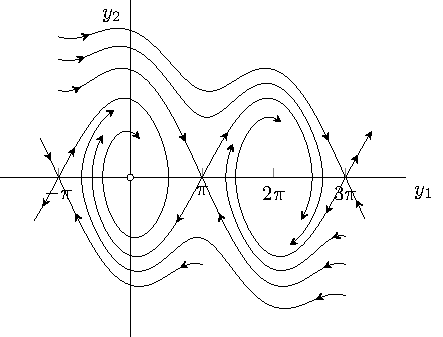
\includegraphics{figSystemPendulumLossyA}
\caption{تقصیری ارتعاش۔مثال \حوالہ{مثال_نظام_دھاگے_سے_لٹکی_کمیت_تقصیری}}
\label{شکل_مثال_نظام_دھاگے_سے_لٹکی_کمیت_تقصیری}
\end{figure}

شکل \حوالہ{شکل_مثال_نظام_دھاگے_سے_لٹکی_کمیت_تقصیری} میں نظام \حوالہ{مساوات_نظام_غیر_خطی_ترکیب_تقصیری_الف} کے خط حرکت دکھائے گئے ہیں۔چونکہ قصری نظام میں توانائی کا ضیاع پایا جاتا ہے لہٰذا شکل \حوالہ{شکل_مثال_نظام_دھاگے_سے_لٹکی_کمیت} کے بند دائروں کی بجائے شکل \حوالہ{شکل_مثال_نظام_دھاگے_سے_لٹکی_کمیت_تقصیری} کے مرغولی خطوط حاصل ہوتے ہیں جو ہمارے توقع کے عین مطابق ہے۔مزید یہ کہ دوری لہری خطوط بھی کسی نہ کسی مقام پر نقطہ فاصل کے گرد گھومنا شروع کر دیتے ہیں۔ اس کے علاوہ اب قصری نظام میں نقطہ زین کو ملانے والے خط نہیں پائے جاتے۔
\انتہا{مثال}
%======================
\ابتدا{مثال}\شناخت{مثال_نظام_شکار_شکاری}\quad آبادی شکار اور شکاری۔ [مسئلہ لوٹکا-ولٹیرا]\\
یہاں لومڑی (شکاری) اور خرگوش (شکار) کی آبادی کے مسئلے پر غور کرتے ہیں۔

\موٹا{پہلا قدم}: ہم فرض کرتے ہیں کہ خرگوش کو جتنی خوراک چاہیے دستیاب ہے۔ یوں لومڑی کی غیر موجودگی میں ان کی تعداد \عددی{y_1'=ay_1} کے تحت قوت نمائی طور پر بڑھے گی۔ لومڑی کی موجودگی میں (اتفاقی آمنے سامنے سے)  خرگوش کی تعداد میں \عددی{y_1y_2} کے راست متناسب کمی پیدا ہو گی۔یوں خرگوش کی تعداد \عددی{y_1'=ay_1-by_1y_2} سے حاصل ہو گی جہاں مستقل \عددی{a>0} اور \عددی{b>0} ہیں۔اسی طرح خرگوش کی غیر موجودگی میں لومڑی کی تعداد \عددی{y_2'=-ly_2} کے تحت قوت نمائی طور پر گھٹے گی۔خرگوش کی موجودگی میں (اتفاقی آمنے سامنے سے) لومڑی کی تعداد \عددی{y_1y_2} کے راست متناسب بڑھے گی۔یوں خرگوش کی موجودگی میں  \عددی{y_2'=-ly_2+ky_1y_2} لومڑی کی تعداد دے گا جہاں مستقل \عددی{l>0} اور \عددی{k>0} ہیں۔

یوں غیر خطی \اصطلاح{مسئلہ لوٹکا-ولٹیرا}\حاشیہد{امریکی ماہر حیاتی طبیعیات الفرڈ جیمز لوٹکا [1880-1949] اور اطالوی ریاضی دان ویٹو ولٹیرا [1860-1940] نے شکار اور شکاری کے مسئلے کو پیش کیا۔} 
\begin{gather}\label{مثال_نظام_شکار_شکاری_الف}
\begin{aligned}
y_1'&=f_1(y_1,y_2)=ay_1-by_1y_2\\
y_2'&=f_2(y_1,y_2)=ky_1y_2-ly_2
\end{aligned}
\end{gather}
حاصل ہوتا ہے۔

\موٹا{دوسرا قدم} مسئلے کو خطی بنانا اور نقطہ فاصل \عددی{(0,0)} کا حصول  ہے۔مساوات \حوالہ{مثال_نظام_شکار_شکاری_الف} کو دیکھ کر نقطہ فاصل مساوات 
\begin{align}
f_1(y_1,y_2)=y_1(a-by_2)=0, \quad f_2(y_1,y_2)=y_2(ky_1-l)=0
\end{align}
کے حل سے \عددی{(y_1,y_2)=(0,0)} اور \عددی{(\tfrac{l}{k},\tfrac{a}{b})} حاصل ہوتے ہیں۔آئیں \عددی{(0,0)} پر غور کریں۔ نقطہ \عددی{(0,0)} کے ہمسائیگی میں مساوات \حوالہ{مثال_نظام_شکار_شکاری_الف} میں \عددی{-by_1y_2} اور \عددی{ky_1y_2} کو نظر انداز کرتے ہوئے خطی نظام
\begin{align*}
\bM{y}'=\begin{bmatrix*}[r] a&0\\0&-l \end{bmatrix*}\bM{y}
\end{align*}
حاصل ہوتا ہے جس کی آئگنی قدر \عددی{\lambda_1=a>0} اور \عددی{\lambda_2=-l<0} کی علامتیں آپس میں الٹ ہیں لہٰذا \عددی{(0,0)} پر نقطہ زین پایا جاتا ہے۔

\موٹا{تیسرا قدم} مسئلے کو خطی بنانا اور نقطہ فاصل \عددی{(\tfrac{l}{k},\tfrac{a}{b})} کا حصول  ہے۔دوسرا نقطہ فاصل \عددی{(y_1,y_2)=(\tfrac{l}{k},\tfrac{a}{b})} پر پایا جاتا ہے۔اس نقطے  کو \عددی{(0,0)} منتقل کرنے کی خاطر ہم \عددی{y_1=\tilde{y}_1+\tfrac{l}{k}} اور \عددی{y_2=\tilde{y}_2+\tfrac{a}{b}} چنتے ہیں۔یوں نقطہ فاصل \عددی{(\tilde{y}_1,\tilde{y}_2)=(0,0)} لکھا جا سکتا ہے۔ چونکہ \عددی{y_1=\tilde{y}_1'} اور \عددی{y_2'=\tilde{y}_2'} ہیں لہٰذا نظام \حوالہ{مثال_نظام_شکار_شکاری_الف} کو درج ذیل لکھا جا سکتا ہے۔
\begin{align*}
\tilde{y}_1'&=\left(\tilde{y}_1+\frac{l}{k}\right)\left[a-b\left(\tilde{y}_2+\frac{a}{b}\right)\right]=\left(\tilde{y}_1+\frac{l}{k}\right)(-b\tilde{y}_2)\\
\tilde{y}_2'&=\left(\tilde{y}_2+\frac{a}{b}\right)\left[k\left(\tilde{y}_1+\frac{l}{k}\right)-l\right]=\left(\tilde{y}_2+\frac{a}{b}\right)k\tilde{y}_1
\end{align*}
نقطہ \عددی{(\tilde{y}_1,\tilde{y}_2)=(0,0)} کے ہمسائیگی میں \عددی{-b\tilde{y}_1\tilde{y}_2} اور \عددی{k\tilde{y}_1\tilde{y}_2} کو نظر انداز کرتے ہوئے خطی نظام
\begin{gather}\label{مثال_نظام_شکار_شکاری_ب}
\begin{aligned}
\tilde{y}_1'&=-\frac{bl}{k}\tilde{y}_2\quad \quad \text{(الف)}\\
\tilde{y}_2'&=\frac{ak}{b}\tilde{y}_1\quad \quad \text{(ب)}
\end{aligned}
\end{gather}
حاصل ہوتا ہے۔مساوات \حوالہ{مثال_نظام_شکار_شکاری_ب}-الف کا بایاں ہاتھ ضرب مساوات-ب کا دایاں ہاتھ برابر ہو گا الف کا دایاں ضرب ب کا بایاں،
\begin{align*}
\frac{ak}{b}\tilde{y}_1'\tilde{y}_1=-\frac{bl}{k}\tilde{y}_2'\tilde{y}_2 \implies \frac{ak}{b}\tilde{y}_1^2+\frac{bl}{k}\tilde{y}_2^2=C
\end{align*}
جس کا تکمل لیتے ہوئے \عددی{\tilde{y}_1} بالمقابل \عددی{\tilde{y}_2} کا \اصطلاح{ترخیمی}\فرہنگ{ترخیم}\حاشیہب{elliptic}\فرہنگ{elliptic} تعلق حاصل کیا گیا ہے۔یوں \عددی{(\tfrac{l}{k},\tfrac{a}{b})} پر شکل \حوالہ{شکل_مثال_نظام_شکار_شکاری} میں دکھایا گیا \اصطلاح{وسط} پایا جاتا ہے۔
\begin{figure}
\centering
\begin{tikzpicture}
%axis
\draw(0,0)--++(4,0)node[right]{$y_1$};
\draw(0,0)--++(0,2)node[left]{$y_2$};
\draw[->-=0.25] ([shift={(0:1cm and 0.5cm)}]2,1) arc  (0:180:1cm and 0.5cm) arc (-180:0:1cm and 0.5cm);
\draw[fill=white](2,1) node[ocirc](kc){};
\draw[dashed] (kc)--(0,1)node[left]{$\frac{a}{b}$};
\draw[dashed](kc)--(2,0)node[below]{$\frac{l}{k}$};
\end{tikzpicture}
\caption{شکار اور شکاری کی آبادی: ماحولیاتی توازن۔}
\label{شکل_مثال_نظام_شکار_شکاری}
\end{figure}

نسبتاً مشکل تجزیے سے ثابت کیا جا سکتا ہے کہ غیر خطی نظام \حوالہ{مثال_نظام_شکار_شکاری_الف} کا \عددی{(\tfrac{l}{k},\tfrac{a}{b})}  پر وسط پایا جاتا ہے البتہ خط حرکت اس نقطے کے گرد غیر ترخیمی بند دائرہ بناتا ہے۔

شکل \حوالہ{شکل_مثال_نظام_شکار_شکاری} کے دائیں کنارے پر خرگوش کی تعداد \عددی{y_1} زیادہ سے زیادہ ہے جس کی وجہ سے لومٹری کی تعداد \عددی{y_2} میں اضافے کی شرح بھی زیادہ سے زیادہ ہے۔اس خط پر گھڑی کی الٹی سمت چلتے ہوئے لومڑی کی زیادہ سے زیادہ آبادی حاصل ہوتی ہے۔اس مقام پر خرگوش کی تعداد اتنی کم ہو چکی ہوتی ہے کہ لومڑی کی بڑھتی تعداد کو خوراک پورا نہیں ہو پایا لہٰذا لومڑی کی آبادی گھٹنے شروع ہو جاتی ہے۔آپ دیکھ سکتے ہیں کہ دونوں جانوروں کی دوری تعداد حالات کے مطابق مسلسل تبدیل ہوتی ہے۔

شکار اور شکاری کی دیگر مثالیں ملخ اور گھاس، ببر شیر اور زیبرا ہیں۔
\انتہا{مثال}
%=====================

